% MAIN DOC
% Example for dissertation.sty
\documentclass[
  % Replace oneside by twoside if you are printing your thesis on both sides
  % of the paper, leave as is for single sided prints or for viewing on screen.
  % oneside,
  twoside=false,
  fontsize=12pt,% NewsGotT
  paper=a4,
  footinclude=true,
  headinclude=true,
  cleardoublepage=empty,
  headsepline=true,
  headheight=20pt,
  footheight=20pt,
  automark,
  markcase=upper,
  bibliography=totoc,
  %appendix=totoc
  %pagestyle=myheadings
  %footsepline=true,
]{scrbook}

% use the formatting style defined (this file should include all other packages)
%\usepackage{./sty/dissertation}% pdflatex
\usepackage{./sty/dissertation-xelatex}% xelatex

% fixing \vbox and \hbox underfull and overfull
% src: https://tex.stackexchange.com/a/387912
\raggedbottom%

%\addtokomafont{section}{\clearpage}
\addtokomafont{caption}{\small}

%this shall be the last thing in the acronym configuration!!
\makeglossaries%

%% **MORE INFO** %%
%to add the acronyms list add the following where you want to print it:
%\printglossary[type=\acronymtype]
%\clearpage
%\thispagestyle{empty}

%to use an acronym:
%\gls{qps}

% Reverse side notes
% How to generate 2 different files based on conditionals
% https://tex.stackexchange.com/a/220101
% see also makefile rule all-comm
\ifdef{\comm}{\reversemarginpar}

% ------------------------------------------------------------------------
% Title
\mytitle% defined in .sty file

% Glossaries & Acronyms
%\makeglossaries  %  either use this ...
%\makeindex	   % ... or this

% Define Acronyms
%%!TEX root = ../dissertation.tex
%
% here are the acronym entries
\newacronym{mei}{MEI}{Mestrado em Engenharia Inform\'{a}tica}
\newacronym{um}{UM}{Universidade do Minho}
\newacronym{di}{DI}{Departamento de Inform\'{a}tica}
%
\newacronym{qos}{QoS}{Quality of Service}
\newacronym{soa}{SOA}{Service Oriented Architecture}
%
\newacronym{oop}{OOP}{Object Oriented Programming}
\newacronym{oose}{OOSE}{Object Oriented Software Engineering}
\newacronym{omt}{OMT}{Object-Modeling Technique}
\newacronym{vdi}{VDI}{Verein Deutscher Ingenieure}
\newacronym{api}{API}{Application Programming Interface}
\newacronym{pwm}{PWM}{Pulse-Width Modulation}
\newacronym{ic}{IC}{Integrated Circuit}
\newacronym{ssr}{SSR}{Solid-State Relay}
\newacronym{pid}{PID}{Proportional Integrative Derivative}
\newacronym{pci}{PCI}{Peripheral Component Interconnect}
\newacronym{pcb}{PCB}{Printed Circuit Board}
\newacronym{io}{I/O}{Input/Output}
%
% ========================== Article_Mach ========================
\newacronym{am}{AM}{Additive Manufacturing}
\newacronym{lbam}{LBAM}{Laser-based Additive Manufacturing}
\newacronym{fgm}{FGM}{Functionally Graded Material}
\newacronym{mmfgm}{MMFGM}{Multi-Material Functionally Graded Material}
\newacronym{mmam}{MMAM}{Multi-Material Additive Manufacturing}
\newacronym{oom}{OOM}{Object-Oriented Modelling}
\newacronym{uml}{UML}{Unified Modeling Language}
\newacronym{sls}{SLS}{Selective Laser Sintering}
\newacronym{slm}{SLM}{Selective Laser Melting}
\newacronym{mmsls}{MMSLS}{Multi-Material SLS}
\newacronym{mms}{MMS}{Multi-Material Sintering}
\newacronym{doe}{DOE}{Design Of Experiments}
\newacronym{ai}{AI}{Artificial Intelligence}
\newacronym{cad}{CAD}{Computer-Aided Design}
\newacronym{cae}{CAE}{Computer-Aided Engineering}
\newacronym{cam}{CAM}{Computer-Aided Manufacturing}
\newacronym{stl}{STL}{Standard Tessellation Language}
\newacronym{amf}{AMF}{Additive Manufacturing File}
\newacronym{3mf}{3MF}{3D Manufacturing Format}
\newacronym{pov}{POV}{Persistence Of Vision}
\newacronym{dlp}{DLP}{Digital Light Projector}
\newacronym{tin}{TIN}{Triangular Irregular Network}
\newacronym{nc}{NC}{Numerical Control}
\newacronym{cnc}{CNC}{Computer Numerical Control}
\newacronym{svg}{SVG}{Scalable Vector Graphics}
\newacronym{html}{HTML}{Hypertext Markup Language}
\newacronym{xml}{XML}{eXtensible Markup Language}
\newacronym{gui}{GUI}{Graphical User Interface}
\newacronym{astm}{ASTM}{American Society for Testing and Materials}
\newacronym{fdm}{FDM}{Fused Deposition Material}
\newacronym{fff}{FFF}{Fused Filament Fabrication}
\newacronym{lom}{LOM}{Laminated Object Manufacturing}
\newacronym{pbf}{PBF}{Powder Bed Fusion}
\newacronym{ded}{DED}{Direct Energy Deposition}
\newacronym{dld}{DLD}{Direct Laser Deposition}
\newacronym{ebm}{EBM}{Electron Beam Melting}
% ================================================================
%
\newacronym{vm}{VM}{Virtual Machine}
\newacronym{lvm}{LVM}{Linux Virtual Machine}
\newacronym{usb}{USB}{Universal Serial Bus}
\newacronym{cli}{CLI}{Command Line Interface}
\newacronym{rtos}{RTOS}{Real-Time Operating System}
\newacronym{ui}{UI}{User Interface}
%
% Final report
\newacronym{qfd}{QFD}{Quality Function Deployment}
\newacronym{sig}{SIG}{Bluetooth Special Interest Group}
\newacronym{ble}{BLE}{Bluetooth Low---Energy}
\newacronym{iot}{IOT}{Internet of Things}
\newacronym{tcp}{TCP}{Transmission Control Protocol}
\newacronym{ip}{IP}{Internet Protocol}
\newacronym{tcpip}{TCP/IP}{Transmission Control Protocol/Internet Protocol}
\newacronym{hci}{Internet Protocol}{Host Controller Interface}
\newacronym{udp}{UDP}{User Datagram Protocol}
\newacronym{rfcomm}{RFCOMM}{Radio Frequency Communications}
\newacronym{l2cap}{L2CAP}{Logical Link Control and Adaptation Protocol}
\newacronym{acl}{ACL}{Asynchronous Connection-Oriented Logical}
\newacronym{sco}{SCO}{Synchronous Connection-Oriented}
\newacronym{psm}{PSM}{Protocol Service Multiplexers}
\newacronym{sdp}{SDP}{Service Device Protocol}
\newacronym{ipc}{IPC}{Inter-Process Communication}
%\newacronym{io}{I/O}{Input/Output}
\newacronym{gprs}{GPRS}{General Packet Radio Service}
\newacronym{gsm}{GSM}{Global System for Mobile Communications}
\newacronym{sms}{SMS}{Short Message Service}
\newacronym{lan}{LAN}{Local Area Network}
\newacronym{sgsn}{SGSN}{Serving GPRS Support Node}
\newacronym{ggsn}{GGSN}{Gateway GPRS Support Node}
\newacronym{ms}{MS}{Mobile Station}
\newacronym{me}{ME}{Mobile Equipment}
\newacronym{sim}{SIM}{Subscriber Identity Module}
\newacronym{dl}{DL}{downlink}
\newacronym{pdp}{PDP}{Packet Data Protocol}
\newacronym{at}{AT}{ATtention}
\newacronym{osi}{OSI}{Open Systems Interconnection}
\newacronym{wlan}{WLAN}{Wireless local Area Network}
\newacronym{os}{OS}{Operating System}
\newacronym{nvs}{NVS}{Navigation Virtual Subsystem}
\newacronym{rvvs}{RVVS}{Remote Vision Virtual Subsystem}
\newacronym{i2c}{I2C}{Inter-Integrated Circuit}
%
%
% Hierarchical structure for MAC
\newglossaryentry{MAC}{name={MAC},description={\nopostdesc}}
\newacronym[parent=MAC]{mac1}{MAC}{Machine Address Code}
\newacronym[parent=MAC]{mac2}{MAC}{Media Access Control}
% ========================== END ======================
%\glsaddall[types={\acronymtype}]

\begin{document}
	% Cover page ---------------------------------------
%	\umfrontcover%	
	\umtitlepage%
%
%% UNUSED - the title should be modified in \mytitle contained in *.sty file

% Title
\titleA{First Part of Title}
\titleB{Second Part of Title} % (if any)
\subtitleA{First Part of Subtitle}
\subtitleB{Second part of Subtitle} % (if any)

% Author
\author{Author of the Thesis}

% Supervisor(s)
\supervisor{The Supervisor of the thesis}
\cosupervisor{The cosupervisor of the thesis}

% University (uncomment if you need to change default values)
% \def\school{Escola de Engenharia}
% \def\department{Departamento de Inform\'{a}tica}
% \def\university{Universidade do Minho}
% \def\masterdegree{Computer Science}

% Date
\date{\myear} % change to text if date is not today

% Keywords
%\keywords{master thesis}

% Glossaries & Acronyms
%\makeglossaries  %  either use this ...
%\makeindex	   % ... or this

% Define Acronyms
%%!TEX root = ../dissertation.tex
%
% here are the acronym entries
\newacronym{mei}{MEI}{Mestrado em Engenharia Inform\'{a}tica}
\newacronym{um}{UM}{Universidade do Minho}
\newacronym{di}{DI}{Departamento de Inform\'{a}tica}
%
\newacronym{qos}{QoS}{Quality of Service}
\newacronym{soa}{SOA}{Service Oriented Architecture}
%
\newacronym{oop}{OOP}{Object Oriented Programming}
\newacronym{oose}{OOSE}{Object Oriented Software Engineering}
\newacronym{omt}{OMT}{Object-Modeling Technique}
\newacronym{vdi}{VDI}{Verein Deutscher Ingenieure}
\newacronym{api}{API}{Application Programming Interface}
\newacronym{pwm}{PWM}{Pulse-Width Modulation}
\newacronym{ic}{IC}{Integrated Circuit}
\newacronym{ssr}{SSR}{Solid-State Relay}
\newacronym{pid}{PID}{Proportional Integrative Derivative}
\newacronym{pci}{PCI}{Peripheral Component Interconnect}
\newacronym{pcb}{PCB}{Printed Circuit Board}
\newacronym{io}{I/O}{Input/Output}
%
% ========================== Article_Mach ========================
\newacronym{am}{AM}{Additive Manufacturing}
\newacronym{lbam}{LBAM}{Laser-based Additive Manufacturing}
\newacronym{fgm}{FGM}{Functionally Graded Material}
\newacronym{mmfgm}{MMFGM}{Multi-Material Functionally Graded Material}
\newacronym{mmam}{MMAM}{Multi-Material Additive Manufacturing}
\newacronym{oom}{OOM}{Object-Oriented Modelling}
\newacronym{uml}{UML}{Unified Modeling Language}
\newacronym{sls}{SLS}{Selective Laser Sintering}
\newacronym{slm}{SLM}{Selective Laser Melting}
\newacronym{mmsls}{MMSLS}{Multi-Material SLS}
\newacronym{mms}{MMS}{Multi-Material Sintering}
\newacronym{doe}{DOE}{Design Of Experiments}
\newacronym{ai}{AI}{Artificial Intelligence}
\newacronym{cad}{CAD}{Computer-Aided Design}
\newacronym{cae}{CAE}{Computer-Aided Engineering}
\newacronym{cam}{CAM}{Computer-Aided Manufacturing}
\newacronym{stl}{STL}{Standard Tessellation Language}
\newacronym{amf}{AMF}{Additive Manufacturing File}
\newacronym{3mf}{3MF}{3D Manufacturing Format}
\newacronym{pov}{POV}{Persistence Of Vision}
\newacronym{dlp}{DLP}{Digital Light Projector}
\newacronym{tin}{TIN}{Triangular Irregular Network}
\newacronym{nc}{NC}{Numerical Control}
\newacronym{cnc}{CNC}{Computer Numerical Control}
\newacronym{svg}{SVG}{Scalable Vector Graphics}
\newacronym{html}{HTML}{Hypertext Markup Language}
\newacronym{xml}{XML}{eXtensible Markup Language}
\newacronym{gui}{GUI}{Graphical User Interface}
\newacronym{astm}{ASTM}{American Society for Testing and Materials}
\newacronym{fdm}{FDM}{Fused Deposition Material}
\newacronym{fff}{FFF}{Fused Filament Fabrication}
\newacronym{lom}{LOM}{Laminated Object Manufacturing}
\newacronym{pbf}{PBF}{Powder Bed Fusion}
\newacronym{ded}{DED}{Direct Energy Deposition}
\newacronym{dld}{DLD}{Direct Laser Deposition}
\newacronym{ebm}{EBM}{Electron Beam Melting}
% ================================================================
%
\newacronym{vm}{VM}{Virtual Machine}
\newacronym{lvm}{LVM}{Linux Virtual Machine}
\newacronym{usb}{USB}{Universal Serial Bus}
\newacronym{cli}{CLI}{Command Line Interface}
\newacronym{rtos}{RTOS}{Real-Time Operating System}
\newacronym{ui}{UI}{User Interface}
%
% Final report
\newacronym{qfd}{QFD}{Quality Function Deployment}
\newacronym{sig}{SIG}{Bluetooth Special Interest Group}
\newacronym{ble}{BLE}{Bluetooth Low---Energy}
\newacronym{iot}{IOT}{Internet of Things}
\newacronym{tcp}{TCP}{Transmission Control Protocol}
\newacronym{ip}{IP}{Internet Protocol}
\newacronym{tcpip}{TCP/IP}{Transmission Control Protocol/Internet Protocol}
\newacronym{hci}{Internet Protocol}{Host Controller Interface}
\newacronym{udp}{UDP}{User Datagram Protocol}
\newacronym{rfcomm}{RFCOMM}{Radio Frequency Communications}
\newacronym{l2cap}{L2CAP}{Logical Link Control and Adaptation Protocol}
\newacronym{acl}{ACL}{Asynchronous Connection-Oriented Logical}
\newacronym{sco}{SCO}{Synchronous Connection-Oriented}
\newacronym{psm}{PSM}{Protocol Service Multiplexers}
\newacronym{sdp}{SDP}{Service Device Protocol}
\newacronym{ipc}{IPC}{Inter-Process Communication}
%\newacronym{io}{I/O}{Input/Output}
\newacronym{gprs}{GPRS}{General Packet Radio Service}
\newacronym{gsm}{GSM}{Global System for Mobile Communications}
\newacronym{sms}{SMS}{Short Message Service}
\newacronym{lan}{LAN}{Local Area Network}
\newacronym{sgsn}{SGSN}{Serving GPRS Support Node}
\newacronym{ggsn}{GGSN}{Gateway GPRS Support Node}
\newacronym{ms}{MS}{Mobile Station}
\newacronym{me}{ME}{Mobile Equipment}
\newacronym{sim}{SIM}{Subscriber Identity Module}
\newacronym{dl}{DL}{downlink}
\newacronym{pdp}{PDP}{Packet Data Protocol}
\newacronym{at}{AT}{ATtention}
\newacronym{osi}{OSI}{Open Systems Interconnection}
\newacronym{wlan}{WLAN}{Wireless local Area Network}
\newacronym{os}{OS}{Operating System}
\newacronym{nvs}{NVS}{Navigation Virtual Subsystem}
\newacronym{rvvs}{RVVS}{Remote Vision Virtual Subsystem}
\newacronym{i2c}{I2C}{Inter-Integrated Circuit}
%
%
% Hierarchical structure for MAC
\newglossaryentry{MAC}{name={MAC},description={\nopostdesc}}
\newacronym[parent=MAC]{mac1}{MAC}{Machine Address Code}
\newacronym[parent=MAC]{mac2}{MAC}{Media Access Control}
% ========================== END ======================
%\glsaddall[types={\acronymtype}]



\ummetadata % add metadata to the document (author, publisher, ...)

%\maketitle % should use a customized title creation
% see: https://en.wikibooks.org/wiki/LaTeX/Title_Creation
  % Add dedication
%  %\chapter*{Dedication}
% src: https://tex.stackexchange.com/a/167529
% see also: .sty file (lines 297-309)
\begin{dedicat}
  %\usefont{T1}{LobsterTwo-LF}{bx}{it}
  % src: https://en.wikibooks.org/wiki/LaTeX/Fonts
  \rmfamily
  {\Large To my parents,}\\
  {\large for always pushing me forward.}
  \par   %% or a blank line
  \vspace{4\baselineskip}
  
  \normalfont
  \emph{"Wir m{\"u}ssen wissen,\\ 
  Wir werden wissen"}\\
  \vspace{\baselineskip}
  David Hilbert, 1930

\end{dedicat}

%%
%% ----------License------
%  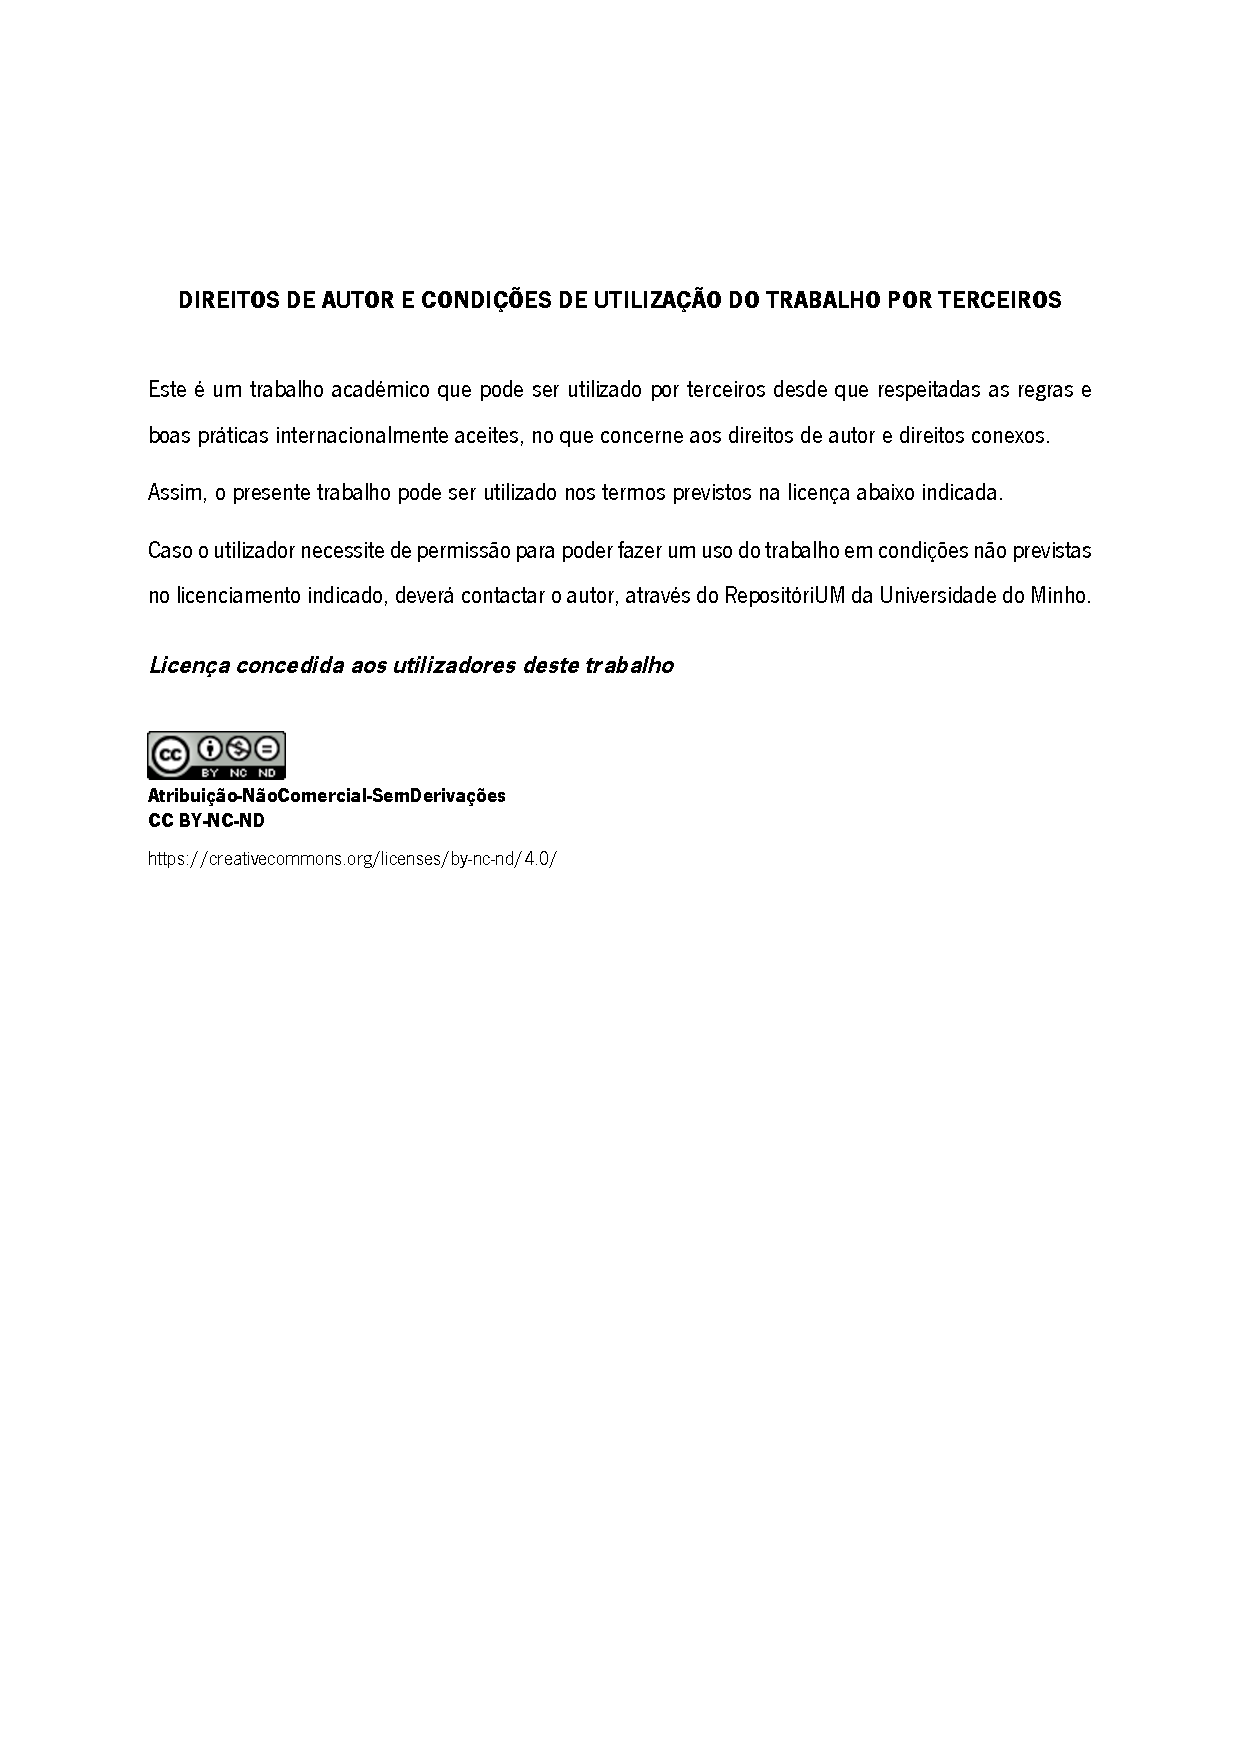
\includepdf[pages=-]{anexo3-license}
%  \cleardoublepage%
%%---------------------
%	% Add acknowledgements ----------------------------
%  \chapter*{Acknowledgements}
First and foremost, I would like to thank...
%%% Local Variables:
%%% mode: latex
%%% TeX-master: "../../dissertation"
%%% End:

%  %\chapter*{Acknowledgements}
%  %	Write acknowledgements here
%  \cleardoublepage%
%%---------------------
%  %
%  \KOMAoption{fontsize}{11.5pt}%
%	% Add abstracts (en,pt) ---------------------------
%  \chapter*{Abstract}
Functional design is the desirable and most sustainable method to design
products: by adding the material only where is strictly required to perform its
function, the resources usage is optimized, especially materials and
energy. However, functional design may dictate the usage of several materials or a combination of them to fulfill its goal, which is hindered by the
current manufacturing methodologies. An example of a class of
products where functional design is key is biomedical implants, like the hip implant.

% Keywords
\keywords{functional design, multimaterial, laser based additive manufacturing}
%%% Local Variables:
%%% mode: latex
%%% TeX-master: "../../dissertation"
%%% End:

%  %\chapter*{Abstract}
%	%Write abstract here (en) or import corresponding file	
%  \cleardoublepage%
%%
%  \KOMAoption{fontsize}{11pt}%
%  \chapter*{Resumo}
\selectlanguage{portuguese}%
O design funcional é o método mais desejável e sustentável de projetar
produtos: adicionando material somente é estritamente necessário para
a sua função, o uso de recursos é otimizado, especialmente materiais e

\keywordspt{design funcional, multimaterial, manufatura aditiva baseada em laser}
\selectlanguage{english}%
%%% Local Variables:
%%% mode: latex
%%% TeX-master: "../../dissertation"
%%% End:

%  %\chapter*{Resumo}
%	%Escrever aqui resumo (pt), ou importar respectivo ficheiro,
%  \cleardoublepage%
	% Summary Lists ------------------------------------
  % add toc and lists to TOC
  % src: https://tex.stackexchange.com/a/74440
%  \KOMAoption{fontsize}{12pt}%
  % TOC
  \phantomsection%
  \addcontentsline{toc}{chapter}{Contents}
  \tableofcontents%
  \cleardoublepage%
  % List of Figs
  \phantomsection%
  \addcontentsline{toc}{chapter}{List of Figures}
  \listoffigures%
  \cleardoublepage%
  % List of Tables
  \phantomsection%
  \addcontentsline{toc}{chapter}{List of Tables}
  \listoftables
  \cleardoublepage%
  % List of listings
  \phantomsection%
  \addcontentsline{toc}{chapter}{List of Listings}
  \lstlistoflistings%
  \cleardoublepage%
  % list of Acronyms
  \phantomsection%
  \addcontentsline{toc}{chapter}{List of Abbreviations}
  \listofacronyms%
  \cleardoublepage%
    %\printglossary[type=\acronymtype]%
    %\printglossary[type=\acronymtype]%
 %   \listofabbreviations%
  % List of symbols
  \phantomsection%
  \addcontentsline{toc}{chapter}{List of Symbols}
  \listofsymbols%
  \cleardoublepage%
%
	\thispagestyle{empty}
  %\newpage
	\pagenumbering{arabic}
  %\newpage
  %\setcounter{page}{0}
  %\pagenumbering{arabic}
  %\setcounter{page}{1}
 % 
  % making chapter pages with no header and footer
  \renewcommand*{\chapterpagestyle}{empty}
  %-------------- MAIN BODY CHAPTERS----------------------------------
  % Include the other files (\include adds a blank page between files)
  % - does not need the file extension
%  \KOMAoption{fontsize}{12pt}%
  \setlength{\unitlength}{1mm}
  %% 1,5 line spacing
  \renewcommand{\baselinestretch}{1.5}
%
  \chapter{Introduction}%
\label{ch:intro}
The envisioned product consists of a remote controlled car used to assist
exploration and maintenance domains, hereby, denominated as Radio Frequency
Camera Assisted Rover (RFCAR). To satisfy such requirements, the vehicle must
contain a remotely operated camera that provides a live video feed to the user.
Additionally, the vehicle must include an odometric system that assists the
driving and avoids unintentional collisions when remote control is compromised, e.g., when connection is lost.
The vehicle provides means for exploration and conditions assessment in critical
or unaccessible areas to human operators, such as fluid pipelines and other
hazardous locations.
The goal of the present work is to close the gap between design and fabrication of
multi-material components from metallic/ceramic materials using
\gls{sls}/\gls{slm} technology. To this end several main objectives have been
outlined:
%
%%% Local Variables:
%%% mode: latex
%%% TeX-master: "../Report"
%%% End:
  \setcounter{table}{0}
  \setcounter{figure}{0}
%
%  %\begin{document}
	% CHAPTER - State of the Art ---------------------
\chapter{State of the art}
\label{ch:state-art}
In this chapter a review on the state of the art is presented. %
Additive manufacturing is discussed briefly as a preliminary topic. %
Then, Laser-based additive manufacturing processes are discussed as viable
solutions for metallic and composite manufacturing. %

%%% Local Variables:
%%% mode: latex
%%% TeX-master: "../../../dissertation"
%%% End:

%  \setcounter{table}{0}
%  \setcounter{figure}{0}
  %
  % CHAPTER - Theoretical foundations ---------------
\chapter{Theoretical foundations}%
\label{ch:theor-found}
In this chapter some background is provided for the main subjects. The
fundamental technical concepts are presented as they proved its usefulness along
the project, namely the project development methodologies and associated tools,
and communications in detail.
%
%\section{Project methodologies}
\section{Project methodologies}
The methodologies used for the project development are briefly described next.
%\subsection{Development methodology of mechatronics --- VDI 2206}
\label{subsec:vdi-2206}

Mechatronics, was defined by Harashima et. al~\cite{harashima1996mechatronics}
as: \emph{''the synergistic integration of mechanical engineering
with electronic and intelligent computer control in the design of industrial
products and processes''}. This definition has more than twenty years, and
nowadays it could be extended to other domains beyond the industrial sector,
but a central idea remains: the synergy between these fields of knowledge, able
% src:
% https://en.wikibooks.org/wiki/LaTeX/Floats,_Figures_and_Captions#Subfloats
\begin{figure}[!hbt]
    \centering
    %\captionsetup[sub]{margin=10pt}
    % a)
    \subcaptionbox{One macro cycle
\label{fig:v-model-macro}}
    [0.5\linewidth]{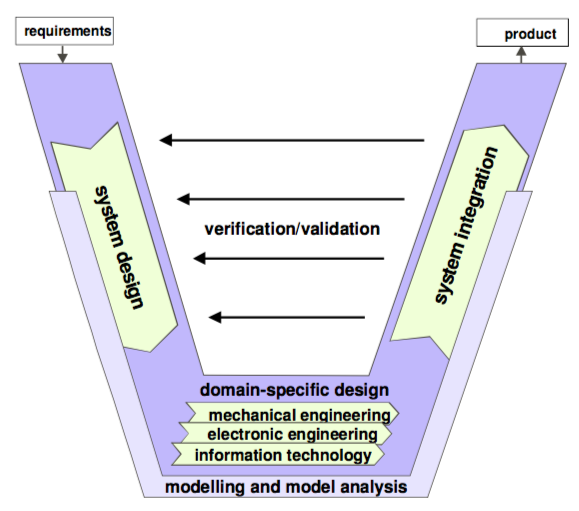
\includegraphics[width=0.45\textwidth]{./img/v-model-macro.png}}
    % b)
    %\subcaptionbox{One macro cycle (refined)~\cite{isermann2008mechatronic} 
    %\label{fig:v-model-isermann}}
    %[0.8\linewidth]{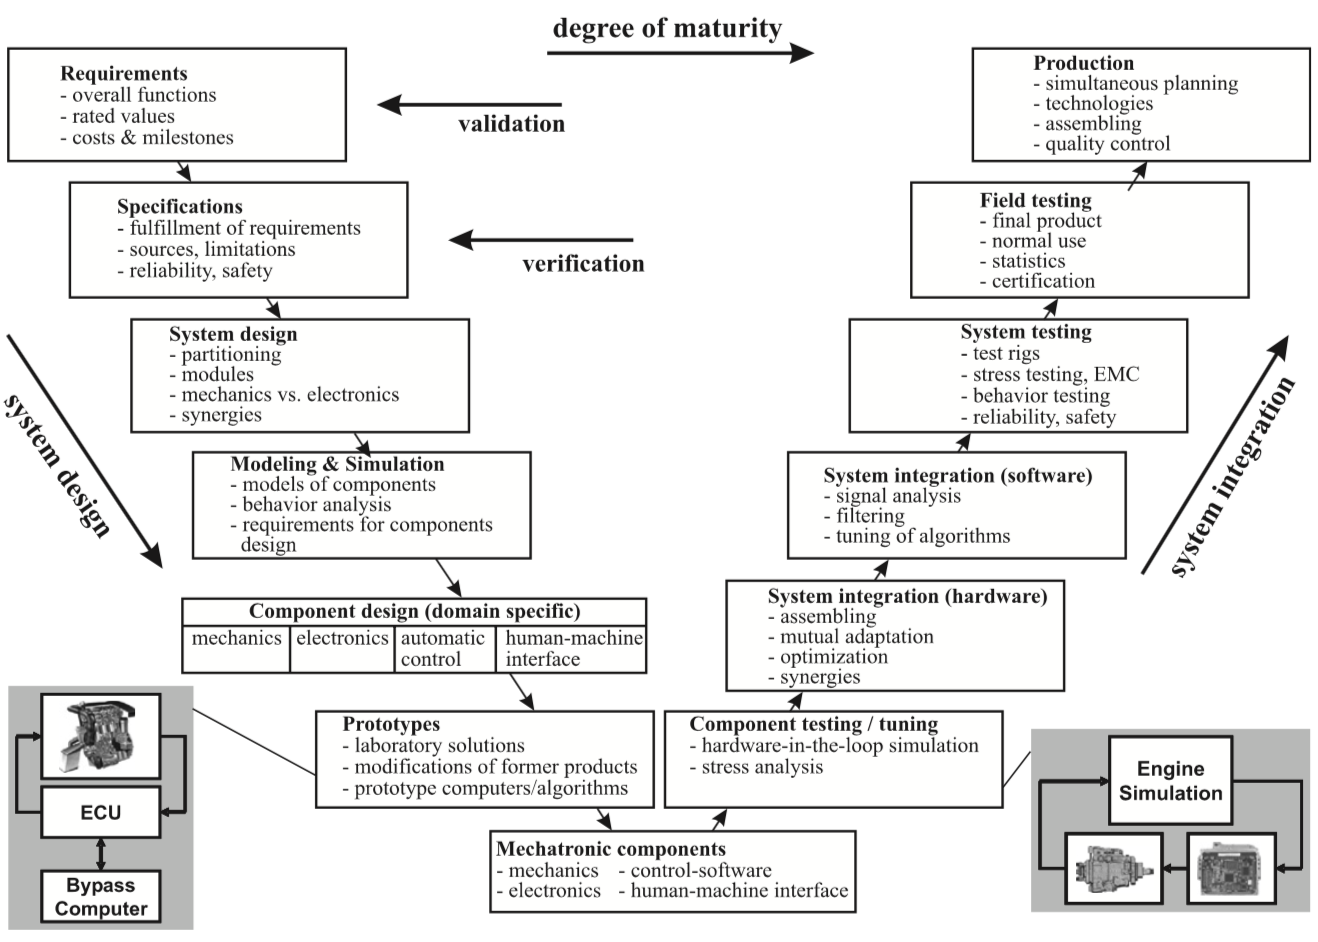
\includegraphics[width=0.8\textwidth]{./img/v-model-isermann.png}}
    % b)
    \subcaptionbox{Iterating over a number of macro-cycles with increasing
      process maturity
\label{fig:v-model-iter}}
    [1.0\linewidth]{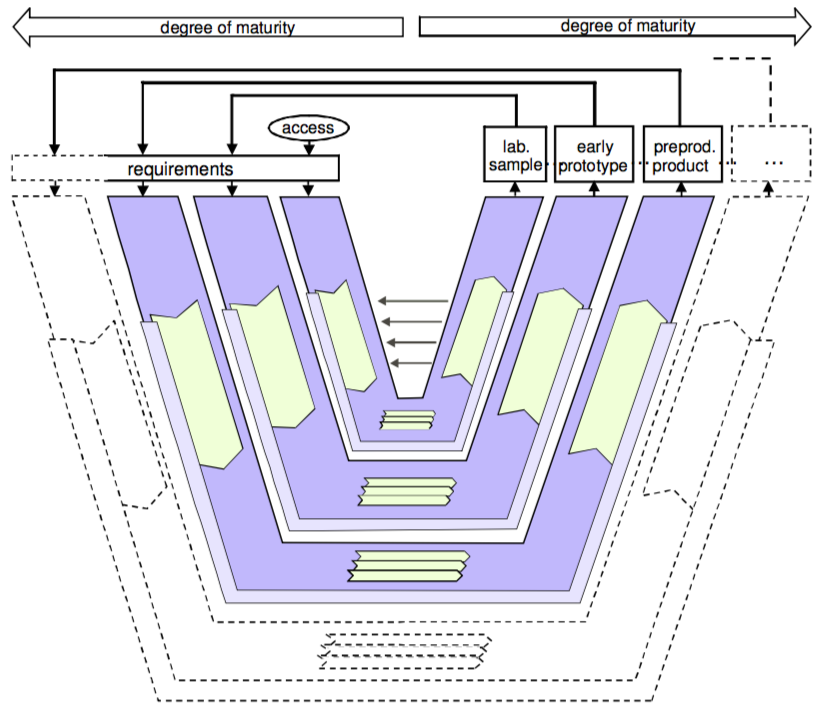
\includegraphics[width=0.55\textwidth]{./img/v-model-iter.png}}
    % c)
    % fig
    \caption{Mechatronics design V-model, VDI 2206 2003~\cite{gausemeier2003new}}
\label{fig:v-model}
\end{figure}

\subsubsection{Process modules for recurrent working steps}
The main phases in the v-model are not yet detailed: this needs to be done by
the designer. However, some design procedures occur regularly during the design
and were identified by field practitioners in terms of predefined process
modules, representing procedures and methods for different design tasks,
organised in a data base
(fig.~\ref{fig:v-model-recurrent}\cite{gausemeier2003new}). The VDI 2206
guideline provides detailed process modules for the V-model macro cycle. One
such example is given in fig.~\ref{fig:v-model-recurrent} for the system design,
which can be described phase-milestone-diagrams, checklists, process-flow
diagrams, etc..

\begin{figure}[!hbt]
  \begin{center}
    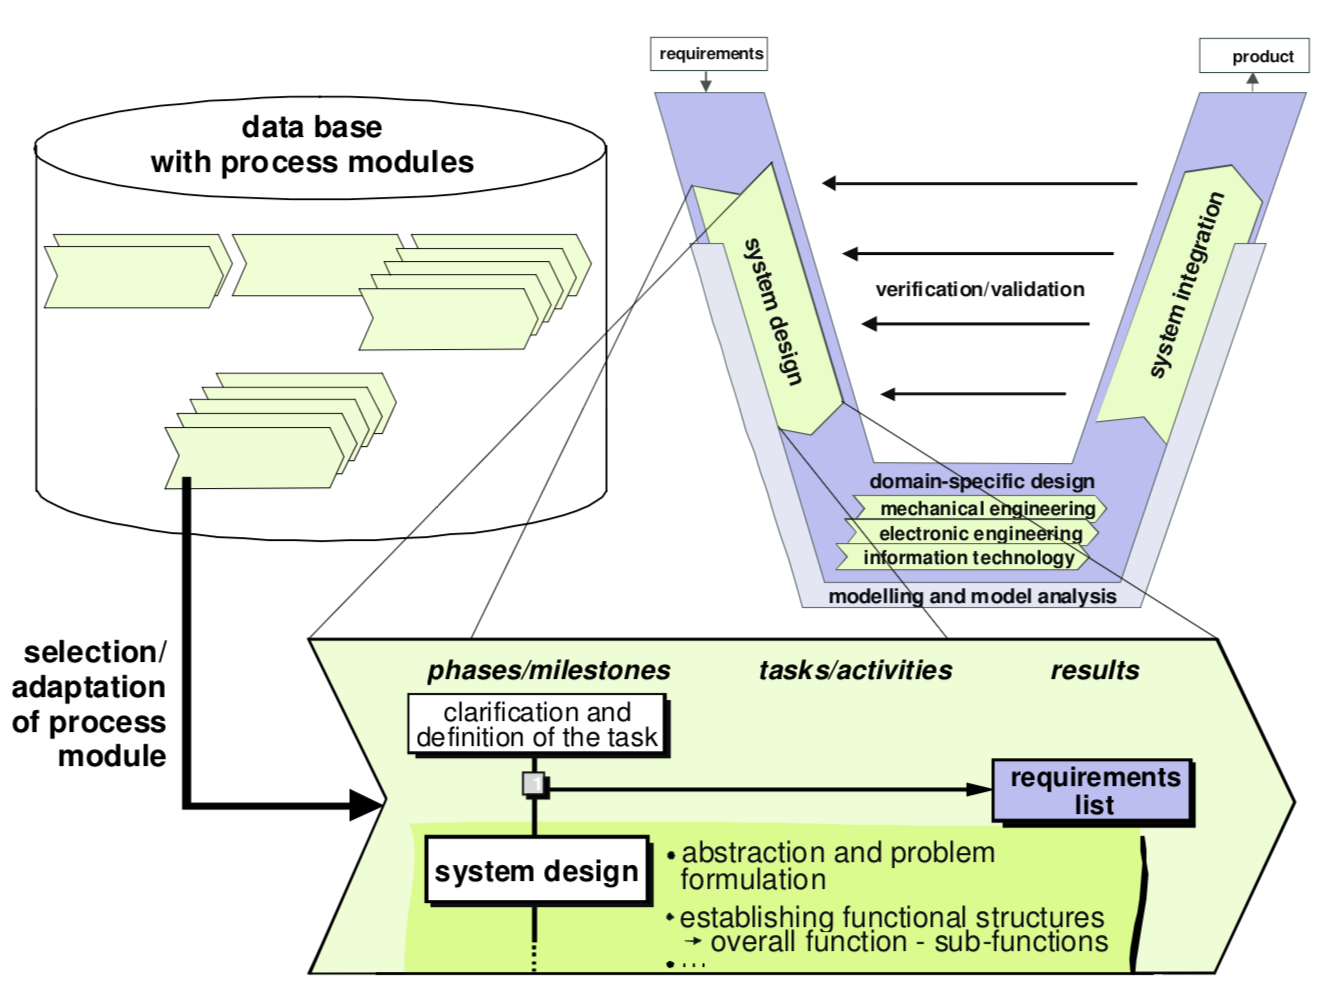
\includegraphics[width=0.65\textwidth]{./img/v-model-recurrent.png}
  \end{center}
  \caption{Configuration of process modules for individual operation steps}
\label{fig:v-model-recurrent}
\end{figure}

%%% Local Variables:
%%% mode: latex
%%% TeX-master: "../../../dissertation"
%%% End:

\subsection{Waterfall}
\label{subsec:waterfall}
For the domain-specific design of software the waterfall methodology is used.
The waterfall model (fig.~\ref{fig:waterfall}) represents the first effort to
conveniently tackle the increasing complexity in the software development
process, being credited to Royce, in 1970, the first formal description of the
model, even though he did not coin the term~\cite{sommerville1996software}. It
envisions the optimal method
as a linear sequence of phases, starting from requirement elicitation to system
testing and product shipment~\cite{cusumano1995beyond} with the process flowing
from the top to the bottom, like a cascading waterfall.

In general, the phase sequence is as follows: analysis, design, implementation,
verification and maintenance.
\begin{enumerate}
  \item Firstly, the project requirements are elicited, identifying the key
    requirements and constraints the system being developed must meet from the
    end-user perspective, captured in natural language in a product requirements document.
  \item In the analysis phase, the developer should convert the application
    level knowledge, enlisted as requirements, to the solution domain knowledge
    resulting in analysis models, schema and business rules.
  \item In the design phase, a thorough specification is written allowing the
    transition to the implementation phase, yielding the decomposition in
    subsystems and the software architecture of the system. 
  \item In the implementation stage, the system is developed, following the
    specification, resulting in the source code.
  \item Next, after system assembly and integration, a verification phase occurs
    and system tests are performed, with the systematic discovery and debugging
    of defects.
  \item Lastly, the system becomes a product and, after deployment, the
    maintenance phase start, during the product life time.
\end{enumerate}
While this cycle occurs, several transitions between multiple phases might
happen, since an incomplete specification or new knowledge about the system,
might result in the need to rethink the document.

The advantages of the waterfall model are: it is simple and easy to understand
and use and the phases do not overlap; they are completed sequentially. However,
it presents some drawbacks namely: difficulty to tackle change and high
complexity and the high amounts of risk and uncertainty. However, in the present
work, due to its simplicity, the waterfall model proves its usefulness and will
be used along the project.

As a reference in the sequence of phases and the expected outcomes from each
one, it will be used the chain of development activities and their products
depicted in fig.~\ref{fig:sw-devel-activities} (withdrawn from
\cite{bruegge2004object}).

\begin{figure}[!hbt]
\centering
    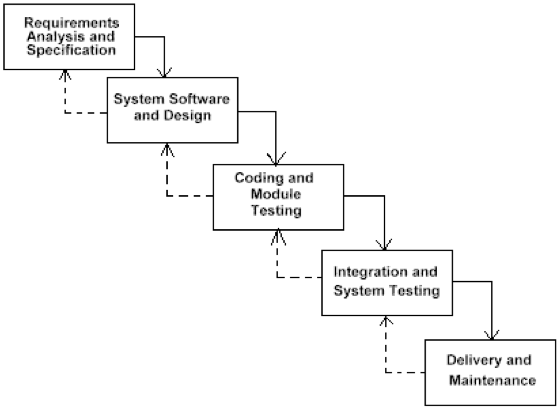
\includegraphics[width=0.6\textwidth]{./img/waterfall.png}
  \caption{Waterfall model diagram}\label{fig:waterfall}
\end{figure}

\subsection{Unified Modeling Language (UML)}
\label{subsec:uml}
To aid the software development process, a notation is required, to articulate
complex ideas succinctly and precisely. The notation chosen was the \gls{uml},
as it provides a spectrum of notations for representing different aspects of a
system and has been accepted as a standard notation in the software
industry~\cite{bruegge2004object}.

The goal of UML is to provide a standard notation that can be used by all
object- oriented methods and to select and integrate the best elements of
precursor software notations, namely \gls{omt}, Booch, and \gls{oose}
~\cite{bruegge2004object}. It provides
constructs for a broad range of systems and activities (e.g., distributed
systems, analysis, system design, deployment). System development focuses on
three different models of the system
(fig.~\ref{fig:sw-devel-activities})~\cite{bruegge2004object}:
\begin{enumerate}
  \item \textbf{\emph{The functional model}}: represented in UML with use case
    diagrams, describes the functionality of the system from the user's point of
    view.
  \item \textbf{\emph{The object model}}: represented in UML with class
    diagrams, describes the structure of the system in terms of objects,
    attributes, associations, and operations.  
  \item \textbf{\emph{The dynamic model}}: represented in UML with interaction
    diagrams, state-machine diagrams, and activity diagrams, describes the
    internal behaviour of the system.
\end{enumerate}

\begin{figure}[!hbt]
\centering
    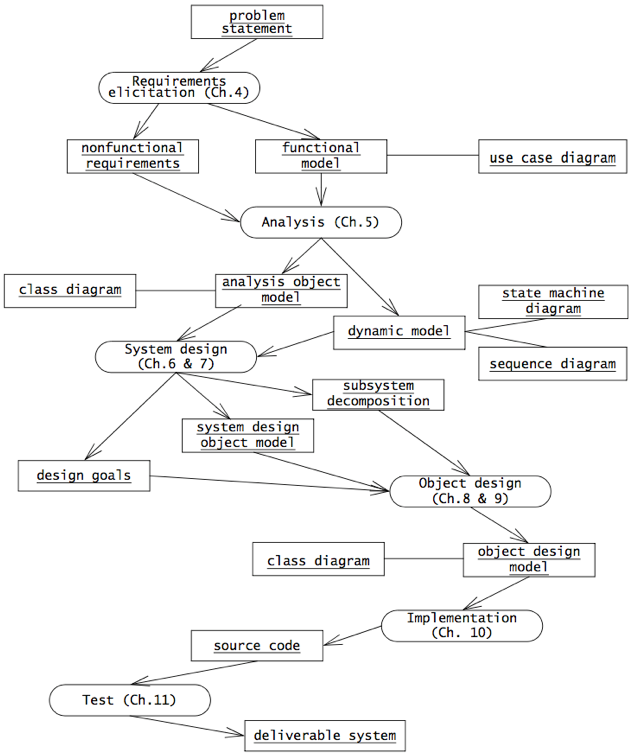
\includegraphics[width=0.7\textwidth]{./img/sw-devel-activities.png}
  \caption{An overview of the object-oriented software engineering development
  and their products. This diagram depicts only logical dependencies among work
  products (withdrawn from~\cite{bruegge2004object})}
\label{fig:sw-devel-activities}
\end{figure}
%%% Local Variables:
%%% mode: latex
%%% TeX-master: "../../../dissertation"
%%% End:

%%% Local Variables:
%%% mode: latex
%%% TeX-master: "../../../dissertation"
%%% End:

%\section{Communications}
% Section: Communications - Handles all communications required for the proj
\section{Communications}
The communications technologies and the associated tools used for the project development are briefly described next.
%
%      % BLUETOOTH
% Bluetooth
\subsection{Bluetooth}%
\label{sec:bluetooth}
Bluetooth is a ubiquituous radio-frequency technology (2.4 GHz) for wireless
communication, generally at short distances. Bluetooth is managed by the
\gls{sig} and the current version of the standard
is 5.0. Starting from version 4.0, also known as \gls{ble}, power consumption
was minimised, making it suitable for embedded and \gls{iot}
applications. Bluetooth is a full protocol stack, illustrated in
Fig.~\ref{fig:ble-stack}, comprising the controller, the host device and the
applications interacting with the device. The \gls{hci} layer enables the host
device to interface the controller, required for low-level operations such as
asynchronous device discovery or reading radio signal intensity. The host
provides profiles to the external applications, easing the interaction betwen
device and applications.
%
\begin{figure}[!hbt]
\centering
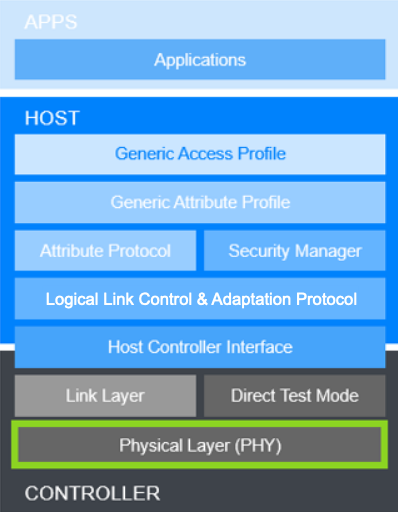
\includegraphics[width=0.45\textwidth]{./img/ble-stack.png}
  \caption{Bluetooth 5.0 protocol stack}%
\label{fig:ble-stack}
\end{figure}
%
Conceptually, Bluetooth is very similar to \gls{tcpip} stack. Both are part of
the network programming class and share the same principles of communication and
data exchange between devices. The difference is that Bluetooth was designed for
short distance communication, whereas the internet programming does not share
this concern. This affects how two devices detect each other initially and how
they establish the initial connection. From that moment on, the procedure is
similar to the \gls{tcpip} stack (see Fig.~\ref{fig:bt-outgoing} and
Fig.~\ref{fig:bt-incoming}).
%
\subsubsection{Establishing a connection}%
\label{sec:bt-establish-conn}
Establishing a connection depends if the device in analysis is trying to
establish an \uline{outgoing} or \uline{incoming} connection. Basically, for the
former case the device sends the first data packet to start the communication,
and for the latter the device receives the first data packet. The devices that
initiate \uline{outgoing} connections must choose a target device and a
transport protocol, before establishing the connection and exchange data. The
devices that initiate \uline{incoming} connections must select a transport
protocol and then \textit{listen} for incoming connections, before establishing
the connection and exchange data~\cite{huang2007bluetooth}.

Figures~\ref{fig:bt-outgoing} and~\ref{fig:bt-incoming} illustrate this concept,
comparing network, internet and bluetooth programming for outgoing and incoming
connections, respectively. For outgoing connections, only the two first steps
(choosing a target device, transport protocol and port number) are different;
after the connection is established, the process is similar. For incoing
connections the procedures are even more similar, with the major difference that
port numbers are dynamically assigned for Bluetooth programming. The procedures
for programming outgoing and incoming connections are presented next.

\uline{Outgoing connection programming procedure}:
\begin{enumerate}
\item Choose a target device
\item Choose a transport protocol and port number
\item Establish a connection
\item Exchange data
\item Disconnect
\end{enumerate}

\uline{Incoming connection programming procedure}:
\begin{enumerate}
\item Choose a transport protocol and port number
\item Reserve local resources and go into listening mode
\item Wait and accept incoming connections
\item Exchange data
\item Disconnect
\end{enumerate}
% Outgoing connections
\begin{figure}[!hbt]
\centering
    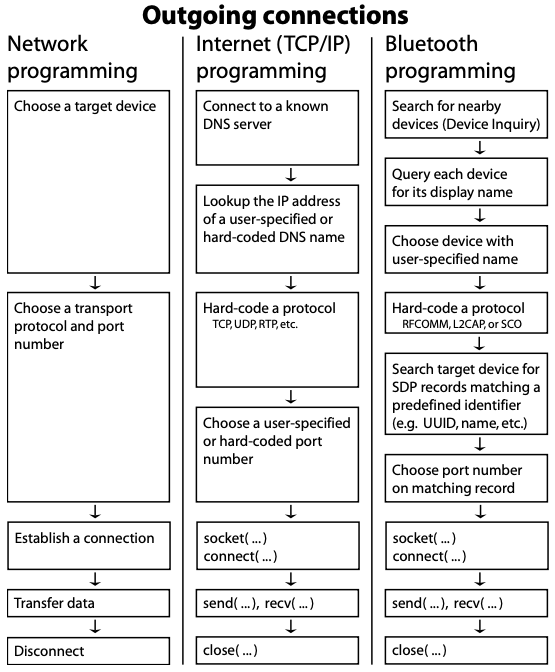
\includegraphics[width=0.47\textwidth]{./img/bt-outgoing.png}
  \caption{Comparison of Network, Internet and Bluetooth programming for
    outgoing connections (withdrawn from~\cite{huang2007bluetooth})}%
\label{fig:bt-outgoing}
\end{figure}
%
%
\begin{figure}[!hbt]
\centering
    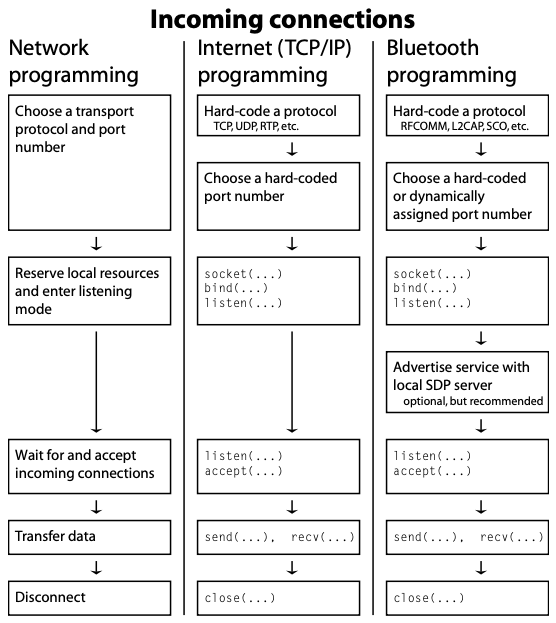
\includegraphics[width=0.47\textwidth]{./img/bt-incoming.png}
  \caption{Comparison of Network, Internet and Bluetooth programming for
    incoming connections (withdrawn from~\cite{huang2007bluetooth})}%
\label{fig:bt-incoming}
\end{figure}
%
\subsubsection{Selecting a target device}%
\label{sec:bt-target-device}
Every Bluetooth chip manufactured has a 48-bit unique address --- BT address ---
identical to the \gls{mac1} for Ethernet protocol, acting as the basic addressing
unit for Bluetooth programming.

The Bluetooth device must know the target device address to
communicate. However, the client application does not need to know \textit{a
  priori} the target address: the end-user provides a user-friendly name ---
\textit{device name} --- and the client translate this to the physical address
when searching for nearby devices. The \textit{device name} may not be unique,
but the address must be.

In the device name lookup process, the device searches for the nearby devices by
inquiring each device individually and compiling a list with their addresses,
which is generally slow. A
Bluetooth device does not announce its presence to other devices; it must start
a device discovery process --- \textit{Device Inquiry} --- to detect them. In
the \textit{Device Inquiry} process the device broadcast a discovery message and
waits for replies. Each reply consists of the physical address of the device and
of an integer identifier the class of the device (e.g., smartphone, headset,
etc.). More detailed information, such as the device name, may be obtained by
contacting each discovered device individually. Additionally, for privacy and
power consumption reasons, the device may choose not to respond to device
inquiries or connections attempts.
%
\subsubsection{Transport protocols}%
\label{sec:bt-transport-protocols}
%
Different applications have different needs, thus the need for different
transport protocols. The two factors that distinguish these protocols are
\textit{guarantees} and \textit{semantics}. The guarantees of a protocol state
how hard it tries to deliver a packet sent by the application, yielding:
\emph{robust} protocols, like \gls{tcp}, which ensures that all sent packets are
delivered or terminates the connection; \emph{best-effort} protocols, like \gls{udp},
which makes a reasonable attempt at delivering transmitted packets, but ignores
its failure. The semantics of a protocol concerns if it distinguishes between
datagrams beginning and end, and can be either packet-based (UDP) or
streams-based (TCP).

Bluetooth contains four essential transport protocols, namely, by relevance
order:
\begin{enumerate}
\item \gls{rfcomm}: reliable and stream-based protocol, which emulates well
  serail ports. It allows only 30 open ports per device and it is the most
  frequently used protocol.
\item \gls{l2cap}: packet-based protocol which can be configured for several
  levels of reliability, imposing delivery order, unlike \gls{udp}. It
  encapsulates the \gls{rfcomm} connection.
\item \gls{acl}: It is not explicitly used, but it encapsulates \gls{l2cap}
  connections. Two Bluetooth devices may have, at most, one \gls{acl} connection
  between them, which is used to transport all \gls{rfcomm} and \gls{l2cap}
  traffic.
\item \gls{sco}: best-effort and packet-based protocol, which is used
  exclusively to transmit voice-quality audio at precisely 64 Kb/s.
\end{enumerate}
The summary of Bluetooth transport protocols is illustrated in
Fig.~\ref{fig:bt-transport-protocols-summary}, where is visibly the connection
encapsulation. Two Bluetooth devices may have, at most, one \gls{acl} and \gls{sco} connection
between them, whereas the number of \gls{rfcomm} and \gls{l2cap} active
connection is limited only by the number of available ports.
% Transport protocols summary
\begin{figure}[!hbt]
\centering
    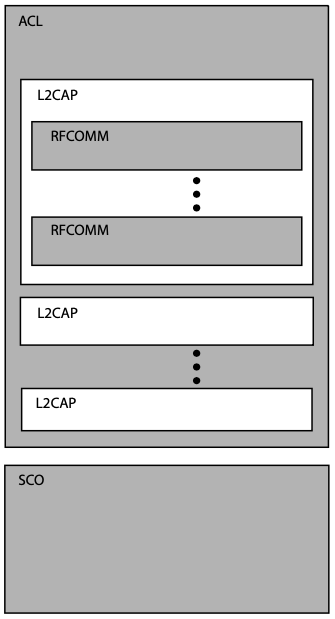
\includegraphics[width=0.3\textwidth]{./img/bt-transport-protocols-summary.png}
  \caption{Most relevant Bluetooth transport protocols (withdrawn from~\cite{huang2007bluetooth})}%
\label{fig:bt-transport-protocols-summary}
\end{figure}
%
\subsubsection{Port Numbers}%
\label{sec:bt-port-nrs}
%
A port is used to enable multiple applications on the same device to use the
same transport protocol. Bluetooth uses a slightly different terminology: for
\gls{l2cap}, ports are called \gls{psm} (range of 1--32767); for
\gls{rfcomm}, ports are called channels (range of 1--30).

Some protocols have a set of reserved/well-known ports, intended for
specific usage. \gls{l2cap} reserves ports 1--1023
for standardized usage (e.g., \gls{sdp} uses port 1), whereas \gls{rfcomm} does
not have reserved ports, given its small number.
\subsubsection{Service discovery}%
\label{sec:bt-service-discovery}
%
For a client application to initiate a outgoing connection it must know in which
port the server application is listening. If the application is standard, then a
reserved port is used. The traditional approach for Internet programming is
hardcoding the same port number at both client and server: when the connection
is established, the server listens on that part and the client connects to
it. However, the static port definition is cumbersome and prevents two server
applications from using the same port.

Bluetooth tries to solve this problem by introducing \gls{sdp}, as illustrated
in Fig.~\ref{fig:bt-sdp-operation}:
\begin{enumerate}
\item Each device keeps an \gls{sdp} server listening on a well-known port.
\item When the server application is executed, it stores a description of itself
  and a port number in the \gls{sdp} server on the local device.
\item Then, when a remote cliente application connects for the first time to the
  device, it provides a description of the service it is searching for, and the
  \gls{sdp} server returns a list of all corresponding services with the
  respective associated port numbers.
\end{enumerate}
% Comparison between connection establishments
\begin{figure}[!hbt]
\centering
    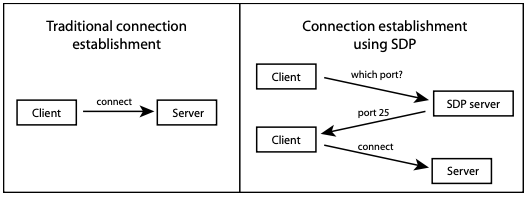
\includegraphics[width=0.6\textwidth]{./img/bt-sdp-operation.png}
  \caption{Comparison between traditional connection establishment (internet)
    and using SDP (Bluetooth) (withdrawn from~\cite{huang2007bluetooth})}%
\label{fig:bt-sdp-operation}
\end{figure}
\subsubsection{Host Controller Interface --- HCI}%
\label{sec:bt-hci}
%
The \gls{hci} defines how a host (e.g., a computer) interacts and communicates
with the local Bluetooth adapter (the controller). All communications between
these two agents are encapsulated in \gls{hci} packets, of four different kinds:
\begin{enumerate}
\item \uline{Command}: sent from the host to the local adapter to control it,
  which can be used for starting a device discovery, connecting to a remote
  device, adjusting the connection parameters, amongst others.
\item \uline{Event}: generated by the local adapter and sent to the host when an
  event of interest occurs, for example, device detected, connection
  established, etc.
\item \uline{ACL data}: encapsulates data to send ou received from a remote
  Bluetooth device. In this sense, the \gls{hci} is a transport protocol for all
  transport protocols (\gls{acl},\gls{l2cap}, and \gls{rfcomm}). When packets
  arrive to the local adapter, the \gls{hci} headers are removed and the pure
  \gls{acl} packet is transmitted through air.
\item \uline{SCO}
\end{enumerate}

\subsubsection{Development Stacks for Bluetooth}%
\label{sec:bt-hci}
%%% Local Variables:
%%% mode: latex
%%% TeX-master: "../../../dissertation"
%%% End:
A development stack refers to a collection of device drivers, development libraries and
tools provided to enable software developers to create Bluetooth
applications. In most operating systems there is a Bluetooth dominant stack,
easing development, as there is a high level of incompatibility between
Bluetooth development stacks. Since Bluetooth is a communications technology,
the transport protocols supported by each stack are of particular
interest. Occasionaly, wrappers around the developed libraries for a stack are
created to provide a higher abstraction programming interface for Bluetooth, in
languages like Python or Java. The most relevant development stacks and wrappers
are depicted in Fig.~\ref{fig:bt-stacks}.
% Bluetooth stacks
\begin{figure}[!hbt]
\centering
    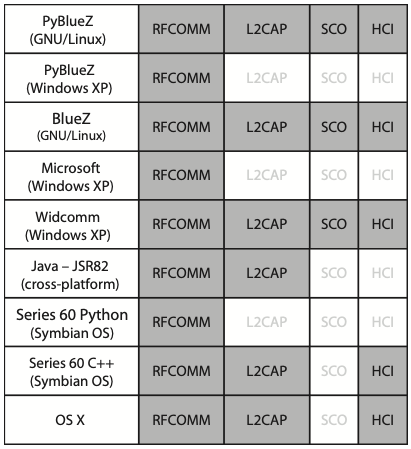
\includegraphics[width=0.4\textwidth]{./img/bt-stacks.png}
  \caption{Most relevant development Bluetooth stacks and wrappers and its
    supported protocols (withdrawn from~\cite{huang2007bluetooth})}%
\label{fig:bt-stacks}
\end{figure}

The Bluetooth development stack selected was \textbf{BlueZ}, since its a
powerful open source stack, included in all major GNU/Linux distributions and
with extensive \gls{api}~s, supporting a extensive set of protocols which
enables to fully explore the Bluetooth local resources. The \gls{rfcomm},
\gls{l2cap}, and \gls{sco} protocols are acessed using the standard sockets
interface and the \gls{hci} is more conveniently used through the provided
wrappers around the several \gls{hci} commands and events.
%
%
%      % WI-FI
%\subsection{Wi-Fi}%
%\label{sec:gprs}
% WIFI
\subsection{IEEE 802.11 --- Wi-Fi}%
\label{sec:wifi}
IEEE 802.11, commonly known as Wi-Fi, is part of the IEEE 802 set of \gls{lan} protocols, and specifies the set of \gls{mac2} and
physical layer protocols for implementing \gls{wlan}
communication in a wide sprectrum of frequencies, ranging from 2.4--60 GHz.

\subsubsection{TCP/IP}%
\label{sec:tcpip}
The most commonly used protocols for Internet communications, including Wi-Fi,
are \gls{tcp} and \gls{ip}, usually associated together, being part of the \gls{osi} model
(Fig.~\ref{fig:osi-model}), which characterises and standardises the
communication functions of a telecommunication or computing system, being
agnostic to their underlying internal structure and technology.

A computer protocol is a standardised procedure for the exchange and
transmission of data between devices, as requested for the application processes.
The TCP provides services at the Transport layer, handling the reliable, unduplicated
and sequenced delivery of data~\cite{carne2004professional}, while the UDP provides data transportation
without guaranteed data delivery or acknowledgments. The TCP can be thought of
a reliable version of \gls{udp}, generalizing. The IP part of the TCP/IP suite, providing
services at the Network layer, is used to make origin and destination addresses
available to route data across networks.

These protocols are applied in sequence to the user's data to create a frame
that can be transmitted from the sending application to the receiving
application.
The receiver reverses the procedure to obtain the original user’s data and pass
them to the receiving application~\cite{carne2004professional}.

Another interesting fact, due to the technology agnostic aspect of the OSI
Model, is that IP and the higher-level protocols may be implemented on several
kinds of physical nets.
% OSI model
\begin{figure}[!hbt]
\centering
    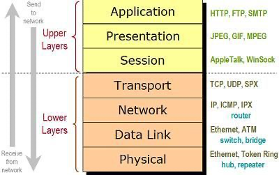
\includegraphics[width=0.5\textwidth]{./img/osi-model.png}
  \caption{\gls{osi} model}%
\label{fig:osi-model}
\end{figure}
%%% Local Variables:
%%% mode: latex
%%% TeX-master: "../../../dissertation"
%%% End:

%      % GPRS
%\subsection{General Packet Radio Service --- GPRS}%
%\label{sec:gprs}
%      % GPRS
\subsection{General Packet Radio Service --- GPRS}%
\label{sec:gprs}
\gls{gprs} is a packet based wireless communication service that offers data
rates from 9.05 up to 171.2 Kbps and continuous connection to the Internet for
mobile phone and computer users~\cite{sanders2003gprs}.
GPRS is based on \gls{gsm} communications and complements existing services such
as circuit switched cellular phone connections and the \gls{sms}.
However, \gls{gprs} is packet oriented (like the Internet), enabling packet data
to be sent to or from a mobile device, closing many of the gaps in the \gls{gsm}
standard, namely~\cite{sanders2003gprs}:
\begin{itemize}
\item enable access to company \gls{lan} and the Internet;
\item provide reasonably high data transmission rates;
\item enable the subscriber to be reachable at all times --- not only for
  telephone calls but also for information such as new emails or latest news:
\item offer flexible access, either for many subscribers at low data rates or
  few subscribers at high data rates, optimizing network usage;
\item offer low cost access to new services
\end{itemize}
A \gls{gsm} network is not able to transmit data in packet switched mode, as
required by \gls{gprs}. Thus, two additional modules were required: \gls{sgsn}
and \gls{ggsn}, yielding the \gls{gsm}/\gls{gprs} network depicted in Fig.~\ref{fig:gprs-network}.
On the user side there is a mobile device known as the \gls{ms}, consisting of a
\gls{me} and the \gls{sim}. For \gls{gprs}, the \gls{me} needs to be equipped
with packet transmission capabilities, constituting three different classes of
\gls{gprs} equipment~\cite{sanders2003gprs}:
\begin{itemize}
\item Class A:~equipment that can handle voice calls and packet data transfers
  at the same time;
\item Class B:~equipment that can handle voice or packet data traffic (but not
  simultaneously) and can put a packet transfer on hold to receive a phone call;
\item Class C:~equipment that can handle both voice and data, but has to
  disconnect from one mode explicitly in order to enable the other.
\end{itemize}
% GPRS network
\begin{figure}[!hbt]
\centering
    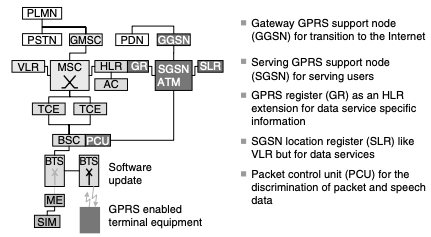
\includegraphics[width=0.5\textwidth]{./img/gprs-network.png}
  \caption{GSM/GPRS network (withdrawn from~\cite{sanders2003gprs})}%
\label{fig:gprs-network}
\end{figure}

The predominant protocol in the world of data networks is the \gls{ip}, enabling
the networking of different network architectures and the standardization of
applications. In the mobile network \gls{gprs} the subscriber has a logical
\gls{ip} connection with an external data network, representing an actual member
of this \gls{ip} network. Packets can then be transferred between the \gls{ms}
and a server in the \gls{ip} network, with the \gls{gprs} standard describing
how they are transmitted on the radio interface and through the whole \gls{gprs}
network.

Prior to the data transfer three important procedures must be
performed~\cite{sanders2003gprs} (see Fig.~\ref{fig:gprs-procedures}):
\begin{enumerate}
\item \uline{gls{gprs} Attach}: the \gls{ms} must be attached in the GPRS network. This is a logical procedure between the \gls{ms} and the \gls{sgsn}
  which takes note of the position, i.e.~the `routing area', of the \gls{ms}. Storing and updating the position of the \gls{ms} is particularly
  important for \gls{dl} transmissions because this information enables the \gls{gprs}
  network to locate the \gls{ms}.
\item \uline{Activation of a \gls{pdp} context}: A
  connection between the \gls{ms} and the \gls{ggsn} must be set up, so each
  node in the GPRS network knows how it has to forward the IP packets of this
  \gls{ms}.
\item \uline{Data transfer}: the path between the MS and the external data network is
  prepared, so IP packets can be sent through the GPRS network towards the
  destination address.
\end{enumerate}
% GPRS network
\begin{figure}[!hbt]
\centering
    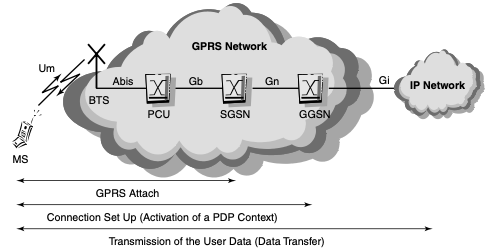
\includegraphics[width=0.65\textwidth]{./img/gprs-procedures.png}
  \caption{GPRS procedures (withdrawn from~\cite{sanders2003gprs})}%
\label{fig:gprs-procedures}
\end{figure}

Thus, the user required hardware for implementation of a GSM/GPRS network is the
\gls{me}, namely, a GSM/GPRS modem and a \gls{sim} card with subscription to a
mobile operator. A GSM/GPRS modem is generally driven through the RS-232 bus,
using the Hayes command set (\gls{at} commands) to interface it.
%%% Local Variables:
%%% mode: latex
%%% TeX-master: "../../../dissertation"
%%% End:

%
%      % SOCKETS
%\subsection{Network programming --- sockets}%
%\label{sec:netw-progr-sock}
%      % SOCKETS
\subsection{Network programming --- sockets}%
\label{sec:netw-progr-sock}
Computer systems implement multiple processes which require an identifier. As
such, the IP address is not enough to uniquely identify the origin/destination
of data to be transmitted, and the port number is added. This combination of an
IP address and port number is sometimes called a network socket~\cite{wright1995tcp}, allowing
data to be delivered to multiple processes in the same machine --- same IP
address.
It is the socket pair (the 4-tuple consisting of the client IP address, client
port number, server IP address, and server port number) that specifies the two
end points that uniquely identifies each TCP connection in an
internet~\cite{wright1995tcp}. Bluetooth, as aforementioned, also uses sockets
for multiprocess communication, given the device address, transport protocol and
port number~\cite{huang2007bluetooth}.

In a broader sense, a socket can be described as a method of \gls{ipc} that allows data to be exchanged between applications, either on
the same host (computer) or on different hosts connected by a network~\cite{kerrisk2010linux}, as a
local interface to a system, created by the applications and controlled by the
operating system, allowing an application process to simultaneously send and
receive messages from other processes.

The Socket API was created in UNIX BSD 4.1 in 1981, with widespread
implementation in UNIX BSD 4.2~\cite{kerrisk2010linux}. It implements the Client-Server paradigm and
implement several (standard) functions to access the operating system network
resources, through system calls, in Linux~\cite{kerrisk2010linux}.

There are two generic ways to use sockets: for outgoing connections --- client
socket --- and for incoming connections --- server
socket. Fig.~\ref{fig:sockets-connection} illustrates the required steps to
obtain a connected socket:
\begin{enumerate}
\item When a socket is initially created is mostly unuseful.
\item Binding the server socket associates it to an unique network tuple (address and
  port number), enabling it to be uniquely addressed.
\item When a socket server goes into listening mode, the remote devices can
  initiate the connection procedure, referring to its unique network tuple.
\item When the socket server accepts a connection, it spawns a new socket which
  is connected to the remote device, and the endpoints can effectively
  communicate. The server socket is ready to accept new incomming connections.
\end{enumerate}
% Sockets connection
\begin{figure}[!hbt]
\centering
    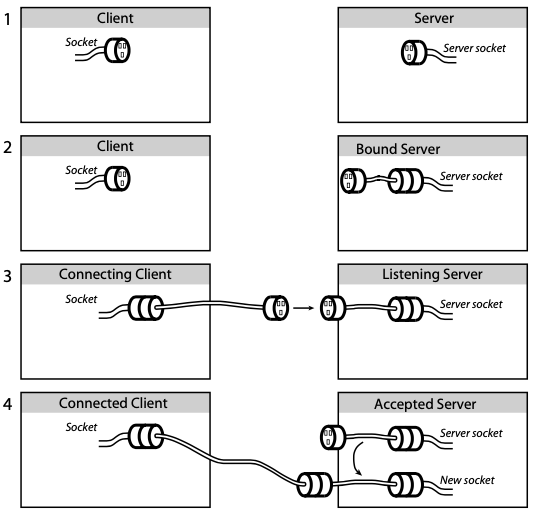
\includegraphics[width=0.4\textwidth]{./img/sockets-connection.png}
  \caption{Steps to obtain a connected socket (withdrawn from~\cite{huang2007bluetooth})}%
\label{fig:sockets-connection}
\end{figure}
%
%%% Local Variables:
%%% mode: latex
%%% TeX-master: "../../../dissertation"
%%% End:

%
%      % CLIENT-SERVER ARCH
%\subsection{Client/server model}%
%\label{sec:client-serv-model}
\subsection{Client/server model}%
\label{sec:client-serv-model}
The client/server model is the most common form of network architecture used
in data communications today~\cite{hanson2000client}. A client is a system or
application that request the activity of a service provider system or
application, called servers, to accomplish specific tasks.
The client/server concept functionally divides the execution of a unit
of work between activities initiated by the end user (client) and resource responses
(services) to the activity request as a cooperative environment~\cite{hanson2000client}. The client,
typically handling user interactions and data exchange/modification in the user’s
behalf, makes a request for a service, and a server, often requiring some resource
management (synchronization and access to the resource), performs that service,
responding to the client requests with either data or status information~\cite{ibmCliServ}.

An example of a simple client-server model using the Socket \gls{api}, through system
calls, is presented in Fig.~\ref{fig:cli-serv-operation}. The operation of sockets can be explained as
follows~\cite{kerrisk2010linux}:
\begin{itemize}
\item The \texttt{socket()} system call creates a new socket, establishing the
  protocols under which they should communicate. For both client and server to
communicate, each of them must create a socket.
\item  Communication via a stream socket is analogous to a telephone call. One
application must connect its socket to another application’s socket before
communication can take place. Two sockets are connected as follows:
\begin{enumerate}
\item One application, assuming the role of server, calls \texttt{bind()} to
  bind the socket to a well-known address, and then calls \texttt{listen()} to
  notify the kernel it is ready to accept incoming connections.
\item The other application, assuming the role of client, establishes the
  connection by calling \texttt{connect()}, specifying the address of the socket
  to which the connection is to be made.
\item The server then accepts the connection using \texttt{accept()}. If the
  \texttt{accept()} is performed before the client application calls
  \texttt{connect()}, then the \texttt{accept()} blocks.
\end{enumerate}
\item Once a connection has been established, data can be transmitted in both
directions between the applications (analogous to a bidirectional telephone
conversation) until one of them closes the connection using \texttt{close()}.
\item Communication is performed using the conventional \texttt{read()} and
  \texttt{write()} system calls or via a number of socket-specific system calls
  (such as \texttt{send()} and \texttt{recv()}) that provide additional
  functionality. By default, these system calls block if the \gls{io} operation
  can’t be completed immediately. However, nonblocking \gls{io} is also
  possible.
\end{itemize}
% Overview of UNIX system calls
\begin{figure}[!hbt]
\centering
    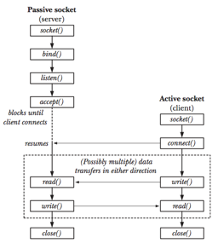
\includegraphics[width=0.4\textwidth]{./img/cli-serv-operation.png}
  \caption{Overview of UNIX system calls with sockets implementing 
a server/client paradigm (withdrawn from~\cite{kerrisk2010linux})}%
\label{fig:cli-serv-operation}
\end{figure}
%
%%% Local Variables:
%%% mode: latex
%%% TeX-master: "../../../dissertation"
%%% End:

%%% Local Variables:
%%% mode: latex
%%% TeX-master: "../../../dissertation"
%%% End:

%\section{Concurrency}
%\label{sec:concurrency}
%      % Concurrency
\section{Concurrency}%
\label{sec:concurrency}
Concurrency is used to refer to things that appear to happen at the same time,
but which may occur serially~\cite{buttlar1996pthreads}, like the case of a multithreaded execution in
a single processor system.
Two concurrent tasks may start, execute and finish in overlapping instants of
time, without the two being executed at the same time.
As defined in POSIX, a concurrent execution requires that a function that
suspends the calling thread shall not suspend other threads, indefinitely.

This concept is different from parallelism. Parallelism refers to the
simultaneous execution of tasks, like the one of a multithreaded program in a
multiprocessor system.
Two parallel tasks are executed at the same time and, as such, they require
the execution in exclusivity in independent processors.

Every concurrent system provides three important facilities~\cite{buttlar1996pthreads}:
\begin{itemize}
\item \textbf{Execution Context}: refers to the concurrent entity state. It
  allows the context switch and it must maintain the entities states,
  independently.
\item \textbf{Scheduling}: in a concurrent system, the scheduling decides what
  context should execute at any given time.
\item \textbf{Synchronisation}: this allows the management of shared resources
  between the concurrent execution contexts.
\end{itemize}
%%% Local Variables:
%%% mode: latex
%%% TeX-master: "../../../dissertation"
%%% End:

%
\section{Android}
\label{sec:android}
The mobile \gls{os} chosen for this project was Android. This section gives an introduction to some android concepts to take into account in section \ref{sec:smartphone-design}. 
%
\subsection{Activity}
\label{sec:activity}
An Android activity  is a view that allows user interaction. Generally, an app can have multiple activities but always starts with the main activity.
Each activity can start another to perform various tasks.

\subsubsection{Activity Lifecycle}
\label{sec:activity_lifecycle}
The activities in the system are managed as activity stacks. The activities are organized in a stack, the back stack, in the order by which they were opened, meaning that when a new activity is started it is placed onto the top of the stack. The prior activity won't come into the foreground unless the current activity exits, e.g., when the user presses a back, home or similar return button.
%
Usually, the lifecycle of an android activity has this four key stages:
\begin {itemize}
\item \textbf {Created}: In this stage the activity is beaing created.
\item \textbf {Resumed}:The activity is in the foreground thus now visible.
\item \textbf {Paused}: Another activity is in foreground but this one is still visible.
\item \textbf {Stopped}: The activity is running in the background and is no longer visible.
\end {itemize}
%
To control this lifecycle, one needs to implement the callback methods that refer to each specific stage by overwriting the pre-existing ones. The lifecycle of an activity is depicted in figure \ref{fig:activity_lifecycle}.
%
\begin{figure}[!ht]
\centering
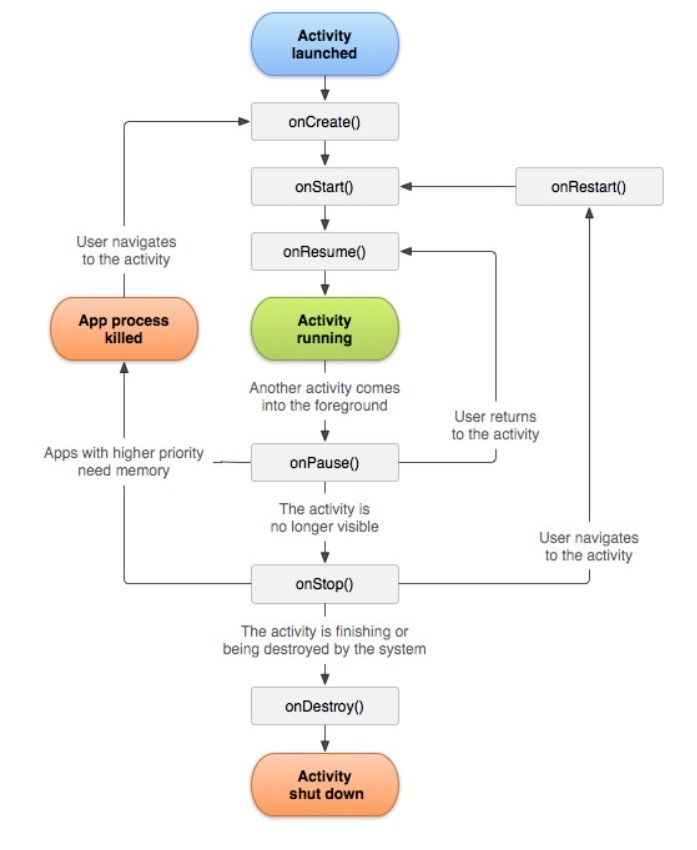
\includegraphics[width =1.0\textwidth]{img/activity_lifecycle.png}
\caption{\label{fig:activity_lifecycle}Android activity lifecycle
view }
\end{figure}
%
%%% Local Variables:
%%% mode: latex
%%% TeX-master: "../../../dissertation"
%%% End:
  \setcounter{table}{0}
  \setcounter{figure}{0}
  %
  % CHAPTER - Requirements Elicitation and Specification definition ------------
\chapter{Requirements Elicitation and Specifications Definition}%
\label{ch:requirements-specs}
In this stage the project requirements are elicited, identifying the key
requirements and constraints the system being developed must meet from the
end-user perspective, captured in natural language in a product requirements
document. The end-user perspective is generally abstract, thus requiring a
methodic approach to obtain well-defined product requirements, i.e., product
specifications. The product specifications are the result of a compromise
between end-user requirements and its feasibility within the available project
resources (time, budget, and technologies available). As the specifications are
well-defined, they serve as design guidelines for the development team and can
be tested later on to assess its feasibility and, ultimately, the quality of the product.
%
%
\section{Foreseen specifications}%
\label{sec:fores-spec}
\section{Foreseen product specifications}%
\label{sec:org31f7574}
In this section the foreseen product specifications of the system to be developed are provided. Such specifications were obtained through the intersection of customer, functional requirements and project restrictions.
\subsection{Quality Function Deployment}%
\label{sec:qfd}
The customer requirements are usually abstract and can collide with the functional requirements, compromising the fulfilment of the project. Thus, it raises the need of a methodology which converts abstract requirements into a series of concrete engineering specifications.

An efficient quality assessment methodology is the use of a Quality House (QFD). In this method, the desired requirements are laid out as rows and the engineering specifications/restrictions as columns. In the intersections lies a symbol representing the strength (weak, moderate or strong --- Figure~\ref{fig:QFD-R} ) of the relationship requirement-specification. This symbol is one of the many tools that allow the quantification of relations existing between the customer requirements and engineering specifications.
For instance, the `engine power' specification and the `fast' requirement have a
very strong correlation (9) since the power of the engine is directly
responsible for the speed of the car.

Along with the requirements, the importance given to each is also specified, ranging from 1 (lowest importance) to 5 (highest importance) these, along with the number at each intersection, will be used to calculate the importance of each specification and thus assign priorities for the Design Team.

Lastly, the triangle shape (the `roof' within the house metaphor) serves as another way of measuring relationships, this time between each specification: such is achieved by placing a symbol (ranging from very negative to very positive, see Figure~\ref{fig:QFD-Roof}) in the diagonal intersection of two specifications. 
I.e., the battery life will have a very negative correlation with the battery temperature, due to the fact that the increase of the temperature will cause a decrease in life time. As such a `very negative' correlation was placed in the diagonal intersection betwixt `Battery Life' and `Battery Temperature'. 
\begin{figure}[!htbp]
   \centering
       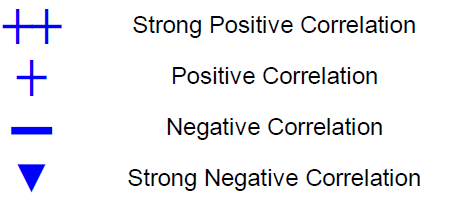
\includegraphics[page=1,width=0.5\textwidth]{sec/img/Roof_Symbols.png} 
 \caption{Quality House - Specification Correlation Strength Symbols}%
\label{fig:QFD-Roof}
\end{figure}

Figure~\ref{fig:QFD} shows the `Quality House' for the RF CAR containing:
\begin{itemize}
\item \textbf{Customer Requirements}: Vehicle Integrity; Obstacle Avoidance; Reliable Feedback; Fast Response; Fast; Budget Friendly; Low Consumption; Small.
\item \textbf{Functional Requirements or Restrictions}: Autonomy; Battery Temperature; Minimum Distance to Obstacle; Maximum Velocity; Motor Expectancy; Cost of Production; Motor Power; Ramp-Up Speed Time; Frame Rate; Camera Range; Resolution; Communication Range; Communication Speed; Dimensions; Mass.
\item \textbf{Intersection Values} (referencing the strength of the requirement-specification correlation) --- see Figure~\ref{fig:QFD-R}.
\item \textbf{Analytical Data}, depicting, in a quantifiable manner, the aims of the project and the relevance of each
  entity:
  \begin{itemize}
  \item Target or Limit Value: The metrics the design team will be based on, white spaces are left for either further discussion and refinement.
  \item Difficulty: Allows a subjective input to be added so that `importance' can be changed to balance unforeseen circumstances.
  \item Importance and Relative Weight: The main conclusion for which the QFD was used, it assigns the priorities for the design team in an objective manner.
  \end{itemize}
\end{itemize}
%
\begin{figure}[!htbp]
   \centering
       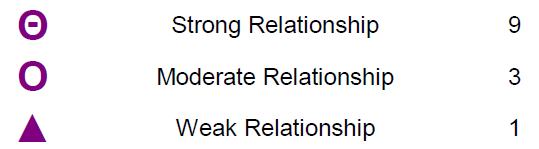
\includegraphics[page=1,width=0.5\textwidth]{sec/img/Relationship_Symbols.png} 
 \caption{Quality House - Relationship Strength Symbols}%
\label{fig:QFD-R}
\end{figure}
%
\begin{sidewaysfigure}[!htbp]
   \centering
       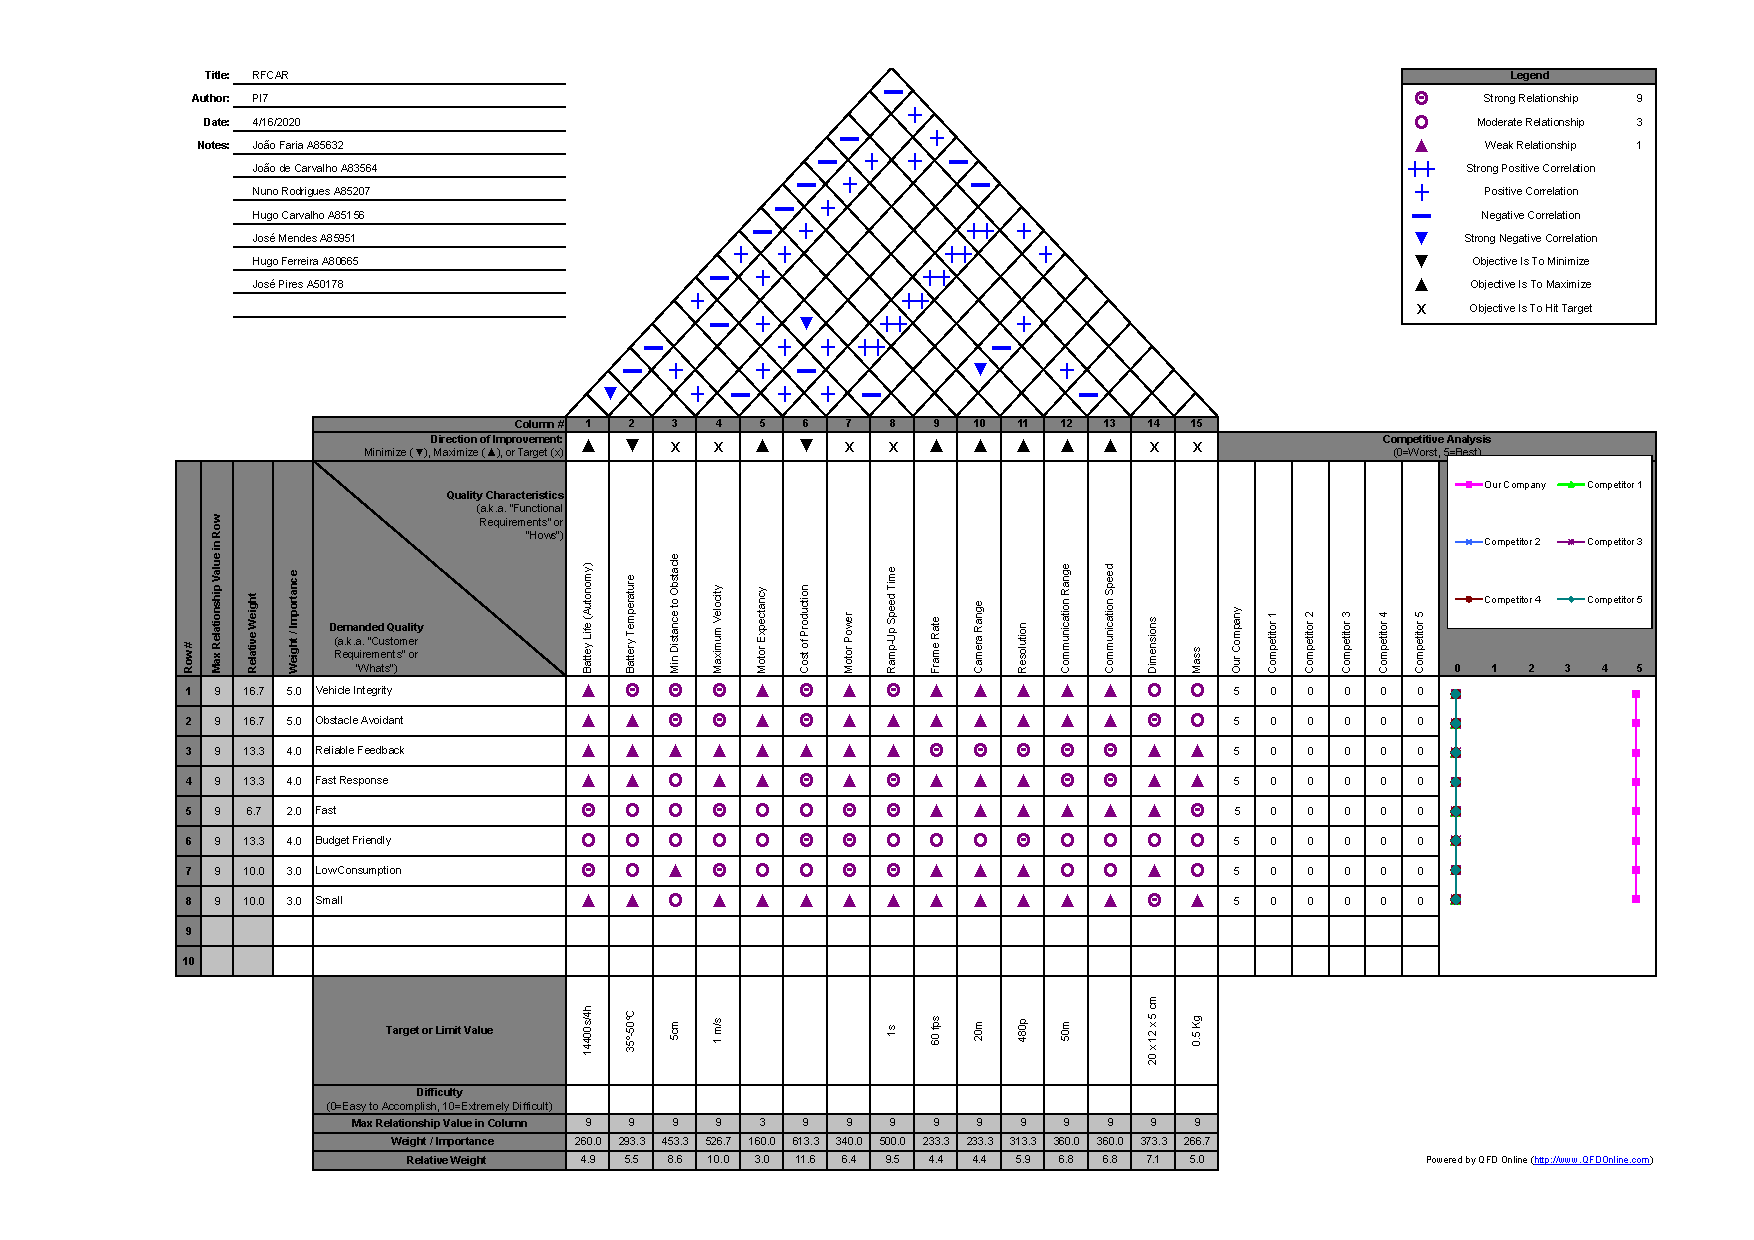
\includegraphics[page=1,width=1.0\textwidth]{sec/pdf/QFDv3.pdf} 
 \caption{Project Study --- RFCar Quality House}%
\label{fig:QFD}
\end{sidewaysfigure}
%
With the QFD, the prioritized ranks and specification targets were obtained and diffused within the Design Team with a
straightforward guideline. For instance, the low cost requirement should be
prioritized over all other specifications, followed by the maximum speed,
Ramp-Up Speed Time and so on.  On the other hand, the engine expectancy is of
little to no consequence (note that the importance added up to a mere 3\%),
followed by the camera-related specifications. This could be regarded as
a point of discussion, which should be prioritized? The functionality of the car
or the the feedback provided by the camera?

With the last point in mind, the QFD has the advantage of promoting further
discussion, simply by changing the importance of a requirement the priority ranking will change, ergo
the priorities can be altered, easily and efficiently, if deemed appropriate.
\newpage
%
\subsection{Vehicle Autonomy}%
\label{sec:autonomy-specs}
The vehicle is operated in wireless mode, thus, a portable power source must be included. The autonomy refers to the vehicle operating hours since the battery is fully charged and safely discharged and should be observed for the following scenarios:
\begin{itemize}
\item No load and vehicle operating at maximum speed;
\item No load and vehicle operating at mean speed;
\item Maximum load and vehicle operating at maximum speed;
\item Maximum load and vehicle operating at mean speed.
\end{itemize}
\subsection{Speed}%
\label{sec:speed-tests}
The vehicle must be operated within a safe range of speed, while also not increasing excessively the power consumption. Thus, these speed boundaries should be tested in the absence of an external load and in the presence of the maximum load.
\subsection{Safety}%
\label{sec:org83942c3}
Vehicle self integrity protection is a requirement in product design, especially considering the vehicle is to
be remotely operated. The safety in the operation can be analysed in two ways, and considers the
preservation of people and goods. For the former, it is important to assure safe interaction as well as user operation --- the vehicle may encounter
several obstacles along its path, but it must not inflict any damage. For the
latter, the vehicle under operating conditions must not inflict any damage to
goods. Thus, in the presence of conflicting user commands violating the safety
of people and goods, the local system should override them, taking corrective
measures to prevent it. The same holds true if the communication between user
and system is lost.
%The system uses odometric navigation.
%\item Human: Due to the odometric sensors safely fixed in the car, crashes will not occur, making it much harder for the car to hit a person or for any part of the car to jump and cause harm to the user or anyone around.
%\end{itemize}
\subsection{Image acquisition}%
\label{sec:image-acquisit}
The vehicle is equipped with a camera to assist in its navigation,
thus, requiring it to be fed to the user's platform appropriately. To do so, several functionalities details need to be addressed efficiently. It was selected the most relevant three and these include the frame rate, the resolution and the image range.
\subsubsection{Frame rate}%
\label{sec:org5adf4ee}
Frame rate refers to the frequency at which independent still images appear on the screen. A better image motion is the result of a higher frame rate but the processing overhead increases as well, so a compromise must be achieved between the quality of the image and the increased processing overhead required. The minimum frame rate defined must be such that allows a clear view of the navigation.
\subsubsection{Range}%
\label{sec:orgecb044c}
How far can the camera capture images without being distorted or unseen by the user. The range must be such that allows the user to see the obstacles when the car is heading to them and provide enough time to change the direction.
\subsubsection{Resolution}%
\label{sec:orgba87554}%
The amount of detail that the camera can capture. It is measured in pixels. The quality of the acquired image is proportional to the number of pixels but a increased resolution requires a greater data transfer and processing overhead, thus, a compromise must be achieved. The minimum resolution must be such that provides the least amount of information required for the user. 
\subsection{Communication}%
\label{sec:org4241610}
For the implementation of the communication, several stages must be considered: Reliability, redundancy and communication range.
\subsubsection{Reliability}%
\label{sec:orgdcb920d}	
A communication is reliable if it guarantees measures to deliver the data
conveyed in the communication link. As reliability imposes these measures, it
also increases memory footprint, which must be considered
depending on the case. For the devised product, an user command
must be acknowledged to be processed, otherwise, the user must be informed; on
the other hand, loosing frames from the video feed is not so critical — user can
still observe conveniently the field of vision if the frame rate is within
acceptable boundaries.
\subsubsection{Redundancy}
\label{sec:orgc5933fc}
The communication protocols are not flawless and the car relies on them to be controlled. If the communication is lost, the car cannot be controlled. A possible solution for this issue is using redundancy in the communication protocols (e.g Wi-Fi and GPRS), so if one protocol fails, the car will still be controlled using the other.
\subsubsection{Range}%
\label{sec:org447a205}
The communication protocols have a limited range of operation, and, as such, regarding the environment on which the car is used the range can be changed.
The range established the maximum distance allowed between user and system for communication purposes.
\subsection{Responsiveness}%
\label{sec:org622e63a}
The movement of the car will be determined by the tilt movement of the smartphone. Sensibility refers to the responsiveness of the car on the minimum smartphone tilt movement. The sensibility must be in an range of values in which small unintentional movements will not be enough to change the state of the car and it does not take big smartphone tilts for the car to move.
\subsection{Closed loop error}%
\label{sec:closed-loop-error-specs}
The speed, direction and safe distance to avoid collisions must be continuously monitored to ensure proper vehicle operation. The closed loop error must then be checked mainly in three situations as a response to an user command:
\begin{itemize}
\item speed: the user issued an command with a given mean speed, which should be compared with the steady-state mean speed of the vehicle.
\item direction: the user issued an command with a given direction, which should be compared to the vehicle direction.
\item safe distance to avoid collisions: the user issued an command with a given direction and speed which can cause it to crash. The local control must influence, to prevent collision, and the final distance to the obstacles must be assessed and compared to the defined one.
\end{itemize}
\subsection{Summary}%
\label{sec:org1f95256}
Table~\ref{tab:specs-init} lists the foreseen product specifications.

% Please add the following required packages to your document preamble:
% \usepackage[table,xcdraw]{xcolor}
% If you use beamer only pass "xcolor=table" option, i.e. \documentclass[xcolor=table]{beamer}
% Please add the following required packages to your document preamble:
% \usepackage[table,xcdraw]{xcolor}
% If you use beamer only pass "xcolor=table" option, i.e. \documentclass[xcolor=table]{beamer}
\begin{table}[!hbt]
\centering
\caption{Specifications}%
\label{tab:specs-init}
%
\begin{tabular}{
>{\columncolor[HTML]{FFFFFF}}l 
>{\columncolor[HTML]{FFFFFF}}l 
>{\columncolor[HTML]{FFFFFF}}l }
\hline
                  & Values     & Explanation                                                                                                  \\ \hline
Autonomy          & 4 h        & \begin{tabular}[c]{@{}l@{}}Time interval between battery fully \\ charged and safely discharged\end{tabular} \\ \hline
Speed Range  & 0.1 to 1 m/s    & \begin{tabular}[c]{@{}l@{}}Speed at which the car can operate\end{tabular}              \\ \hline
Frame Rate        & 60 fps     & \begin{tabular}[c]{@{}l@{}}Frequency at which independent still \\ images appear on the screen\end{tabular}  \\ \hline
Camera Range      & 20 m       & \begin{tabular}[c]{@{}l@{}}How far can the camera capture images\\ without loosing resolution\end{tabular}   \\ \hline
Camera resolution & 480p       & Amount of detail that the camera can capture                                                                 \\ \hline
Communication Range & 50 m & \begin{tabular}[c]{@{}l@{}}Maximum distance between the car and the\\ smarphone without losing connection\end{tabular} \\ \hline
speed Error    & 5 \%       & \begin{tabular}[c]{@{}l@{}}Maximum difference between desired \\ and real speed\end{tabular}              \\ \hline
Direction Error   & 5\%        & \begin{tabular}[c]{@{}l@{}}Maximum difference between desired\\  and real direction\end{tabular}             \\ \hline
Distance Error     & 5 \% & \begin{tabular}[c]{@{}l@{}}Maximum difference between desired\\ and real distance to the obstacle\end{tabular}         \\ \hline
Dimensions        & 20x12x5 cm & Dimensions of the car                                                                                        \\ \hline
Weight            & 0.5 kg     & Weight of the car                                                                                            \\ \hline
\end{tabular}
\end{table}

%%% Local Variables:
%%% mode: latex
%%% TeX-master: "../Phase1"
%%% End:

%

%%% Local Variables:
%%% mode: latex
%%% TeX-master: "../../../dissertation"
%%% End:

  \setcounter{table}{0}
  \setcounter{figure}{0}
%  	% CHAPTER - Problem and Challenges ---------------
\chapter{The problem and its challenges}
\label{ch:prob-challenge}
  The multi-material part fabrication is a complex topic and most current
  commercially available systems have been designed for mono-material part
  fabrication~\cite{wohlers2011wohlers} and are unprepared for multi-material
  processing due to the lack of flexibility and processing capability. 

  \chapter{Analysis}%
\label{ch:analysis}
The envisioned product consists of a remote controlled car used to assist
exploration and maintenance domains, hereby, denominated as Radio Frequency
Camera Assisted Rover (RFCAR). To satisfy such requirements, the vehicle must
contain a remotely operated camera that provides a live video feed to the user.
Additionally, the vehicle must include an odometric system that assists the
driving and avoids unintentional collisions when remote control is compromised, e.g., when connection is lost.
The vehicle provides means for exploration and conditions assessment in critical
or unaccessible areas to human operators, such as fluid pipelines and other
hazardous locations.
%
%%% Local Variables:
%%% mode: latex
%%% TeX-master: "../Report"
%%% End:


  \setcounter{table}{0}
  \setcounter{figure}{0}
  %
  % CHAPTER - Design ---------------
\chapter{Design}%
\label{ch:design}
In the design phase, the solution is developed in the various domains and a
thorough specification is written, paving the way for implementation. In this
chapter is presented the design for the various domains and subsystems identified.

\section{Navigation Virtual Subsystem}%
\label{sec:navig-virt-subsyst-design}
The Navigation subsystem hosts the core of the system functionality-wise, which is the control routine. This means that it should strive to not only make accurate readings and calculations but also be as efficient as possible in managing those processes in order to introduce very little delay and meet timing requirements. 

To meet these requirements as best as possible it should be capable of :

\begin{itemize}
    \item Gathering information from the physical domain at equally distant instants $kT_s$ and output an electrical representation of the command variable at equally distant instants $kT_o$;
    \item Acquiring commands from the Smartphone and Remote Vision Subsystems, identifying matches that will allow it to validate those commands and feeding them into the control rule in a useful format;
    \item Providing real-time feedback to the user about its status.
\end{itemize}


The first task should be idealizing the control system itself, understanding what inputs are needed to control the machine and then how it could be used to manipulate the wheels of the car. After that, the rest of system should be designed to fit the needs of the control rules and algorithms and use them to react as fast and consistently as possible within its own constraints and those of the other subsystems.
%
\subsection{Control}%
\label{sec:control-design}
The objective of the control module is to be capable of, with an input reference velocity and steering angle, outputting the appropriate command variables to achieve said references. The first step in its design is to conceptualize the car's model; since the interest lies in the motion of the car, the kinematic model will be the one to be studied.
\subsubsection{Conception Of Car Model}
\label{sec:concep}

\begin{figure}[!htbp]
\centering
       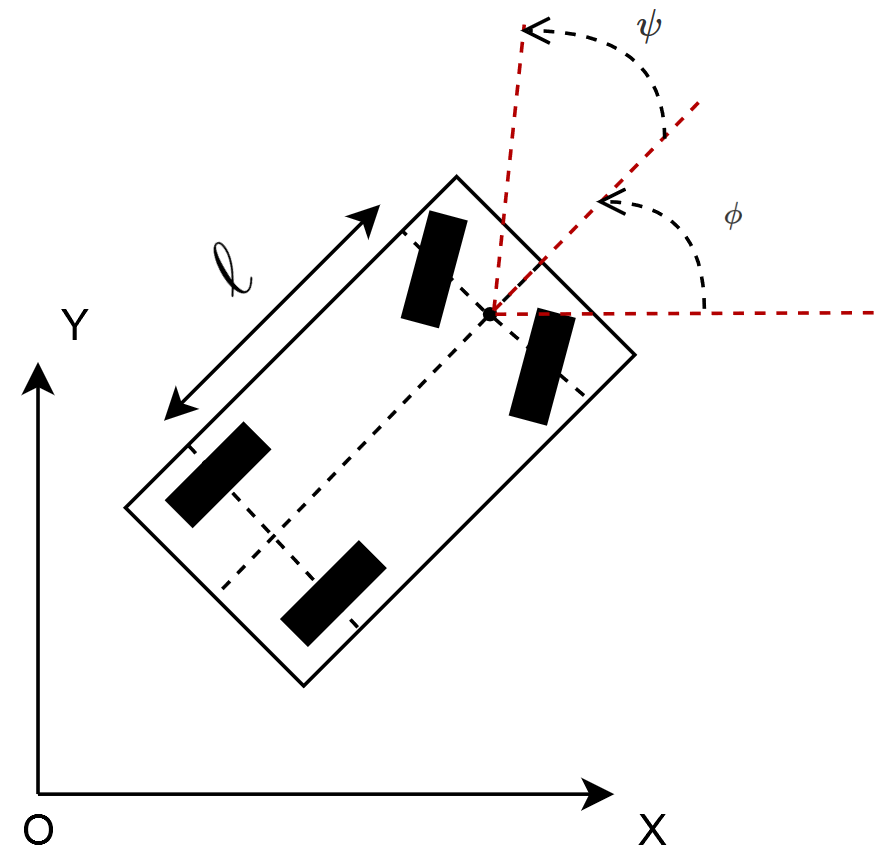
\includegraphics[page=1,width=0.6\textwidth]{img/kinematicModel.png} 
\caption{Kinematic Model of Car}
\label{fig:kinModel}
\end{figure}

Considering the kinematic model of a four-wheel vehicle with a wheelbase length $\ell$, a linear velocity v(t) and an angular velocity $\omega(t)$ the following situation will occur: since the rear wheels will remain in the same position no matter where the car is facing towards, they will be facing whatever orientation, $\phi$, the car is facing, however, in order for the car to be capable of moving into wherever the user tells it to, the front wheels must turn, ergo a steering angle $\psi$, must be considered. The resulting direction the car will be going in is $\phi + \psi$. With these considerations, a desired angle of tilt $\theta$ and considering that $\phi=0$, in other words, that whatever direction the car is told to face, it will be relative to its current direction, the following model is obtained:
\begin{align}
\dot{x}&=v(t) cos(\psi)\\
\dot{y}&=v(t) sin(\psi)\\
\dot{\psi}&=\omega(t)=\frac{v(t)}{\ell}\theta
\end{align}
However this model is not enough for simulation purposes. The simulation has the objective of granting the designers clear ideas of the response of the systems towards given inputs, therefore, for implementation purposes, the simulation must give feedback on the position of the car, its heading and the linear velocity of the right rear wheel ($v_r$), and the left rear wheel ($v_l$) therefore the model will have to changed with these details in mind, which can be achieved considering that:
\begin{align}
\omega(t)&=\frac{v_r(t)-v_l(t)}{\ell}\\
v(t)&=\frac{1}{2}(v_r(t)+v_l(t))
\end{align}
Solving the system above for $v_r$ and $v_l$:
\begin{align}
v_ r(t)&=v(t)+ \frac{\omega(t)\ell}{2}\\
v_l(t)&=v(t)-\frac{\omega(t)\ell}{2}
\end{align}
Returning the model in order to $\dot{x}$ and $ \dot{y}$:
\begin{align}
\dot{x}&=v(t) cos(\psi)-\frac{\ell}{2}\omega(t) sin(\psi)\\
\dot{y}&=v(t) sin(\psi)+\frac{\ell}{2}\omega(t) cos(\psi)\\
\dot{\psi}&=\omega(t)=\frac{v(t)}{\ell}\theta
\end{align}
\subsubsection{Simulation Model}
The mathematical model determined in Section~\ref{sec:concep} was simulated in
the Matlab/Simulink environment. Converting the mathematical model into a
simulink subsystem yields (Fig.~\ref{fig:carModel}):
\begin{figure}[!htbp]
\centering
       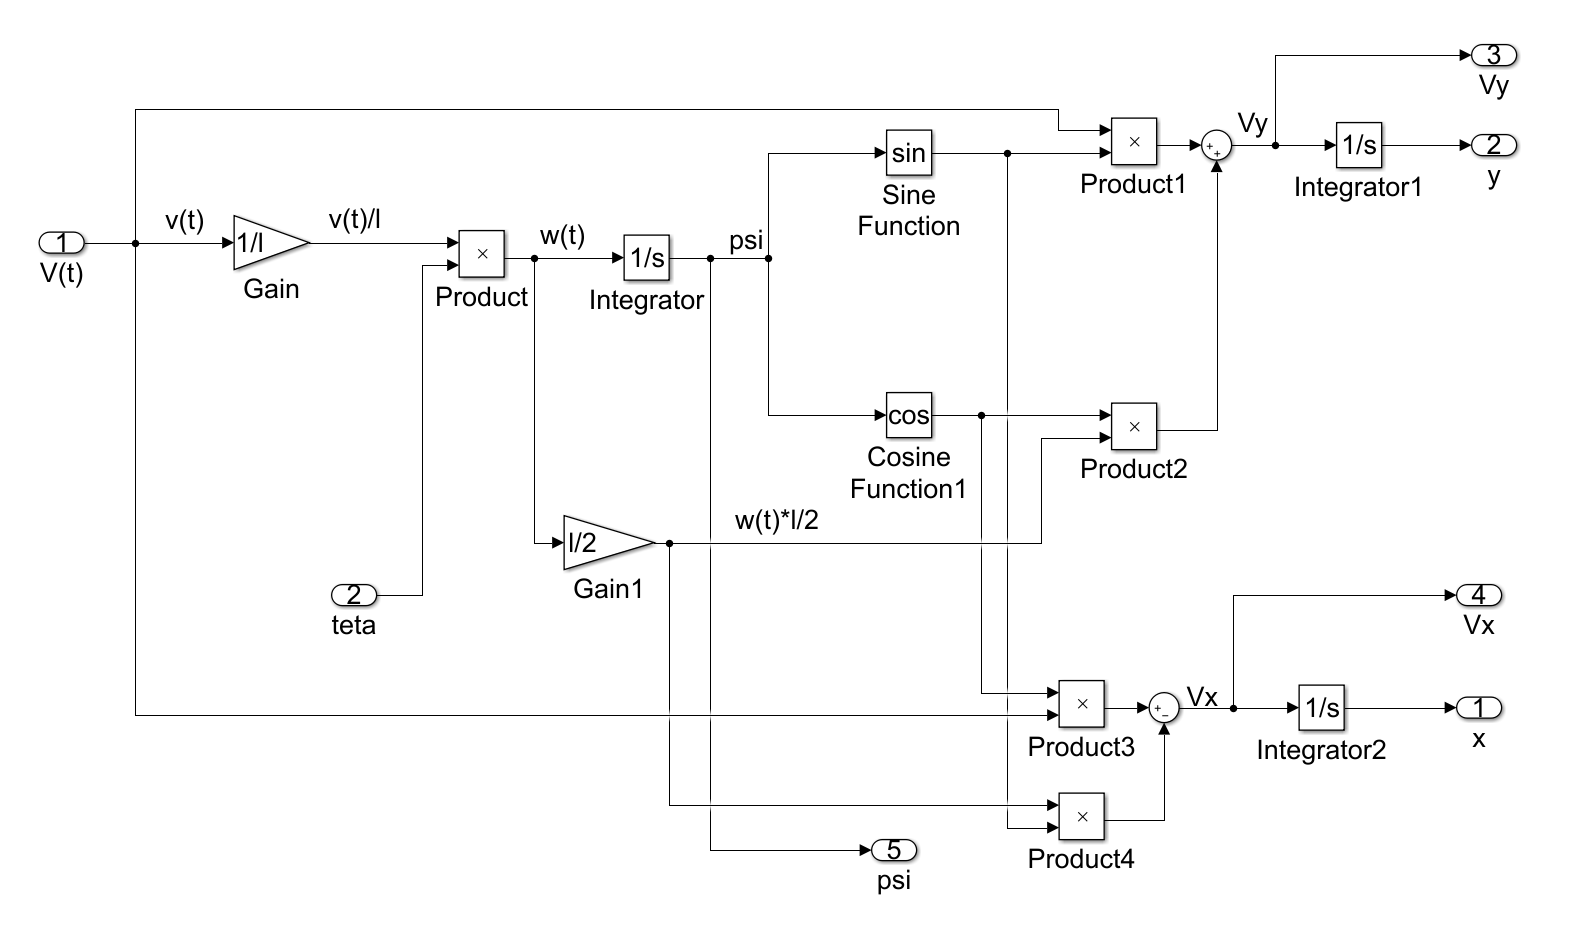
\includegraphics[page=1,width=1\textwidth]{img/subsystem.png} 
\caption{Car Model in a Simulink Subsystem}%
\label{fig:carModel}
\end{figure}
After obtaining the model of the car, the control simulations of the system may begin:
\begin{figure}[!htbp]
\centering
       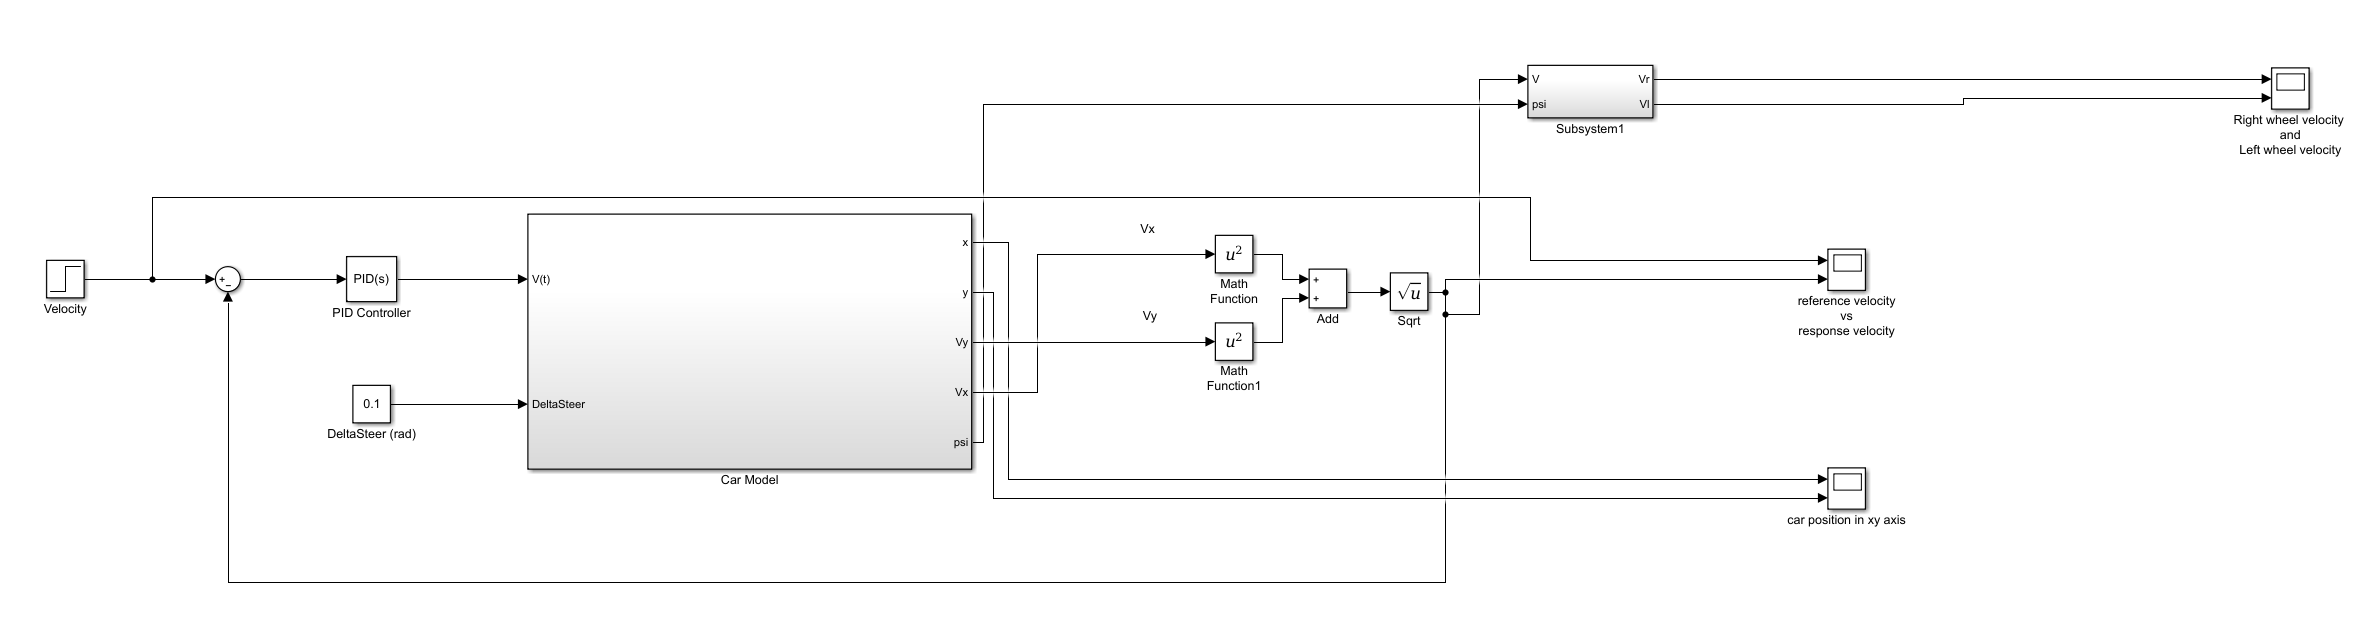
\includegraphics[page=1,width=1\textwidth]{img/system.png} 
\caption{Simulation Schematic}
\end{figure}\\
The simulation schematic uses the model in Fig.~\ref{fig:carModel} within the
`Car Model' subsystem to simulate the response of the system to a step reference
of the desired velocity and a constant reference of the angle to which the car
should turn towards. It calculates the norm of the velocity vector, returns it
as feedback and also uses it to pass through subsystem1 that will return the
different velocities at which each of the rear wheels must turn in order to
achieve said angle.
%%% Local Variables:
%%% mode: latex
%%% TeX-master: "../../../dissertation"
%%% End:

%SUBSECTION - control
\subsubsection{Discrete PID}
\label{sec:des-pid}

To control the system, a PID controller was used for the reason that it is the most used of all controllers in this type of cases and also leads to better system behavior because of the following statements : the proportional action defines the velocity of approach to the value in steady state; the integral action reduces the error in steady state by integrating the error; the derivative action anticipates the response, deriving the error, allowing to reduce the oscillatory behavior of the system response and its integration in the controller should always be analysed, principally in systems with a lot of noise, to avoid instability in the system.\\
The PID controller can be implemented either in analog or digital, however, the implementation it is usually digital using a system with a microprocessor associated. This method can also improve the performance by allowing control of actuator saturation(wind-up), even in systems with a lot of noise in the measured variables. Thus, the digital control system performs the sampling of inputs of interest, calculates the value of the control variable and then, if necessary, convert it to an analog value. The sampling introduces a delay in the system and keep the entry value between consecutive samples, leading to the concept of retainer. Normally, the Zero Order Holder (ZOH) is selected to model this effect in the control.\\

The analog PID controller equation is given by Eq. \ref{equ:pid-analog}:
\begin{equation}
\label{equ:pid-analog}
C(t) = C_{est} + K_c\bigg(e(t) + \frac{1}{\tau_i} \int e(t')dt' + \tau_d \frac{de(t)}{dt}\bigg)
\end{equation}
\begin{itemize}
\item C(t): control action
\item \(C_{est}\): control action in steady state;
\item \(K_c\): proportional controller gain;
\item \(\tau_i\): integral time constant;
\item \(\tau_d\): derivative time constant;
\item \(r(t) = y_r(t) - y(t)\): error, given by the difference between reference and the output of the system.
\end{itemize}

The discrete PID controller equation is obtained by discretizing the Eq. \ref{equ:pid-analog} term to term in moments \(n\) and \(n-1\), resulting in
Eq. \ref{equ:pid-discrete}, called position algorithm:
\begingroup
\small
\begin{equation}
\label{equ:pid-discrete}
C[n] = C_{est} {+} K_c\bigg(e[n] {+} \frac{T}{\tau_i} \sum_{i=0}^n e[i] + \tau_d \frac{e[n]{-}e[n {-} 1]}{T}\bigg)
\end{equation}
\endgroup
\begin{itemize}
\item C[n]: control action
\item \(C_{est}\): control action in steady state;
\item \(K_c\): proportional controller gain;
\item \(\tau_i\): integral time constant [s];
\item \(\tau_d\): derivative time constant [s];
\item \(e[n] = y_r[n] - y[n]\): error, given by the difference between reference and the output of the system for instant n.
\item \(e[n{-}1]\): error for instant n-1.
\item \(T\): sampling period [s]
\end{itemize}
Determining the equivalences for the earnings of the controller in the most conventional one: 
\begin{equation}
\label{equ:pid-discrete-params}
K_p = K_c;~K_i = K_c\frac{T}{\tau_i};~K_d = K_c \frac{\tau_d}{T}
\end{equation}

There are other algorithms for PID control, namely the speed algorithm and the modified ones (position and speed). The speed algorithm calculates the variation of the controller output signal in relation to the immediately previous moment, presenting advantages over position algorithm as it does not need initialization and protects against eventual saturation of the controller (wind-up) and against computational failures. The modified algorithms aim to mitigate the derivative jump when there is an abrupt change in the error, by applying the derivative action to the measured variable instead of the error.\\

To the modified speed algorithm will then come:
\begin{equation}
\label{equ:pid-discrete-veloc-modif}
\begin{split}
C[n] = C[n-1] + K_c\bigg((y_m[n{-}1]-y_m[n]) + \frac{T}{\tau_i} e[n] \\ + \tau_d \frac{{-} y_m[n] {+} 2 y_m[n{-}1] {-} y_m[n{-}2] }{T}\bigg)
\end{split}
\end{equation}



	

%SUBSECTION - control
\subsubsection{Optimal control parameters determination}
As the controller in use is a discrete PID, the first step is to find the optimal parameters.
For the first set of simulations, the aim is to find the values for the PID gains. As purpose of the car is to explore hazardous areas, the parameter Kd will be set as 0 due to the noise. 
For the first simulation, $K_d = 1$, $K_i = 1$, Linear speed = 1 m/s, $\theta =
0~\si{rad}$:
\begin{figure}[!h]
\centering
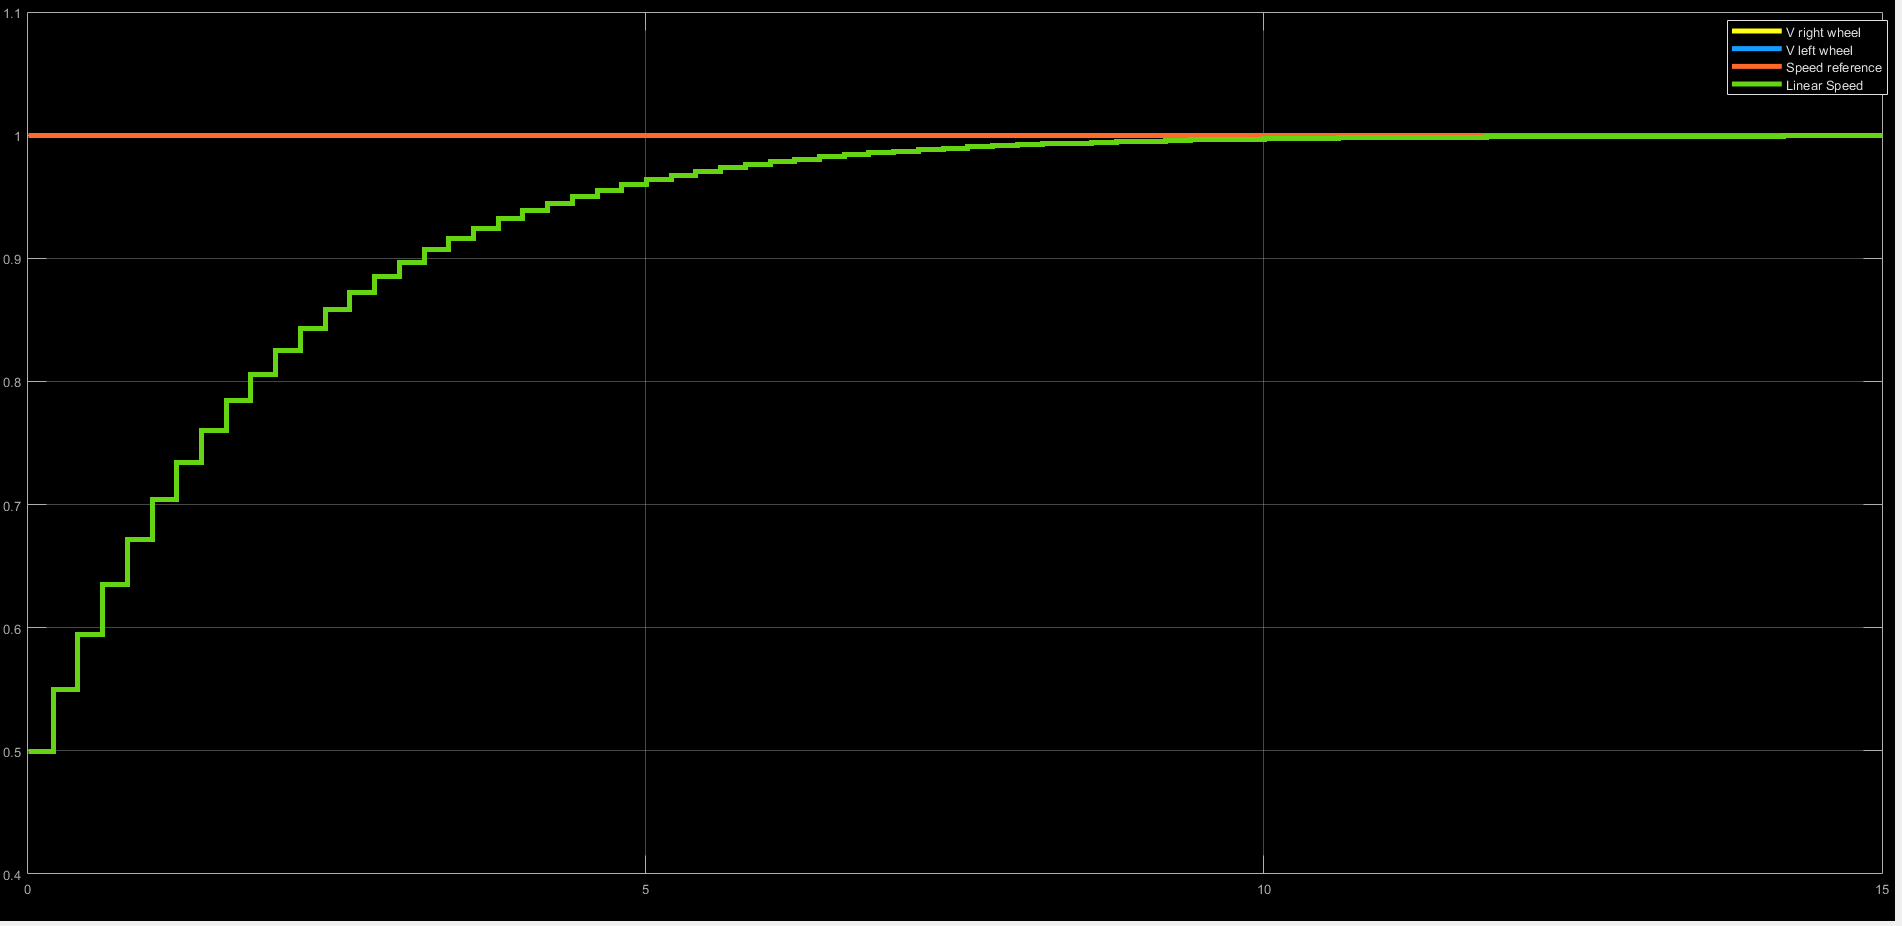
\includegraphics[width=1.0\textwidth]{./img/pid11.png}
\caption {\label{fig:pid1-p1i1}Kp=1, Ki=1}
\end{figure}
With this simulation, it is possible to see that the initial value of the velocity of the car is 0.5 m/s and it take about 7 seconds to reach steady state. 0.5m/s as an initial value for the linear velocity is a considerably high value and can cause the car to slide, therefore, the Kp value needs to get lower, for the initial value to get lower as well.
%\newpage
In this simulation, Kp will be set as 0.5 and Ki as 1.
\begin{figure}[!h]
\centering
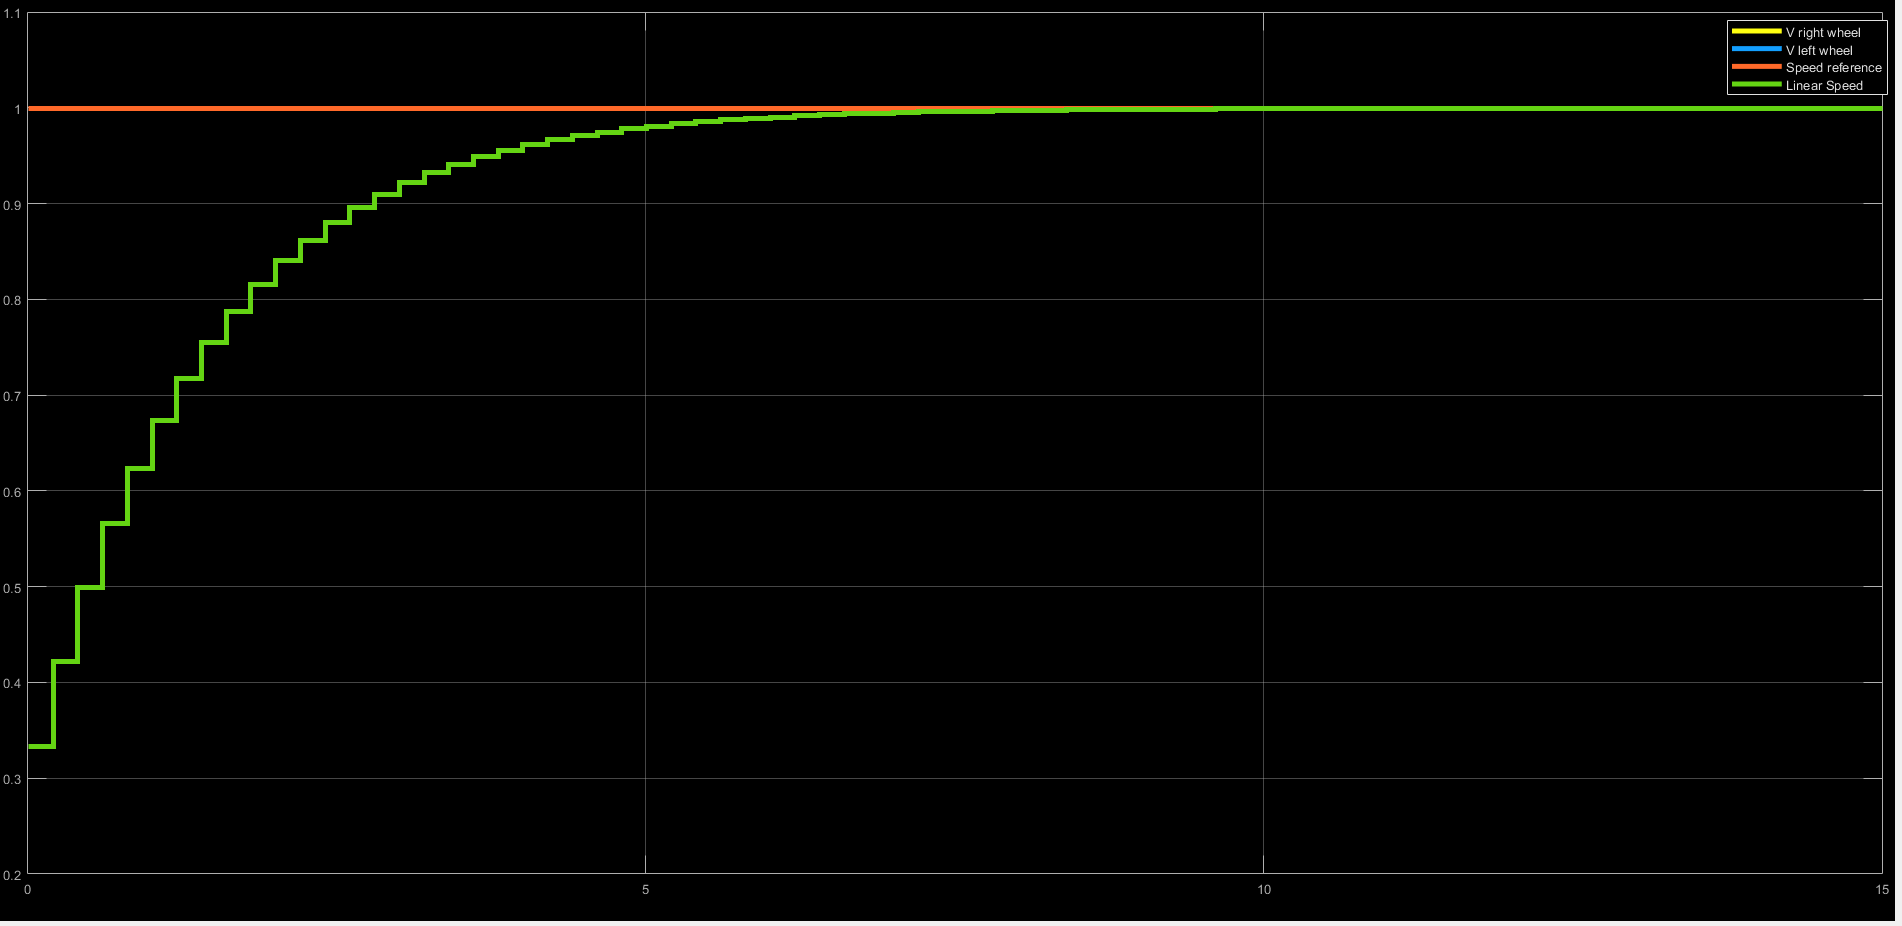
\includegraphics[width=1.0\textwidth]{./img/pid051.png}
\caption {\label{fig:pid1-p05i1}Kp=0.5, Ki=1}
\end{figure}
Changing the value of Kp to half of the initial value, it is possible to see that the initial linear speed is now 0.3 m/s, making it harder for the car to slide. It takes nearly 6 seconds for the car to reach steady state, thus the Ki value must be increased.
%\newpage
In this simulation, Kp will be set as 0.5 and Ki as 2.
\begin{figure}[!h]
\centering
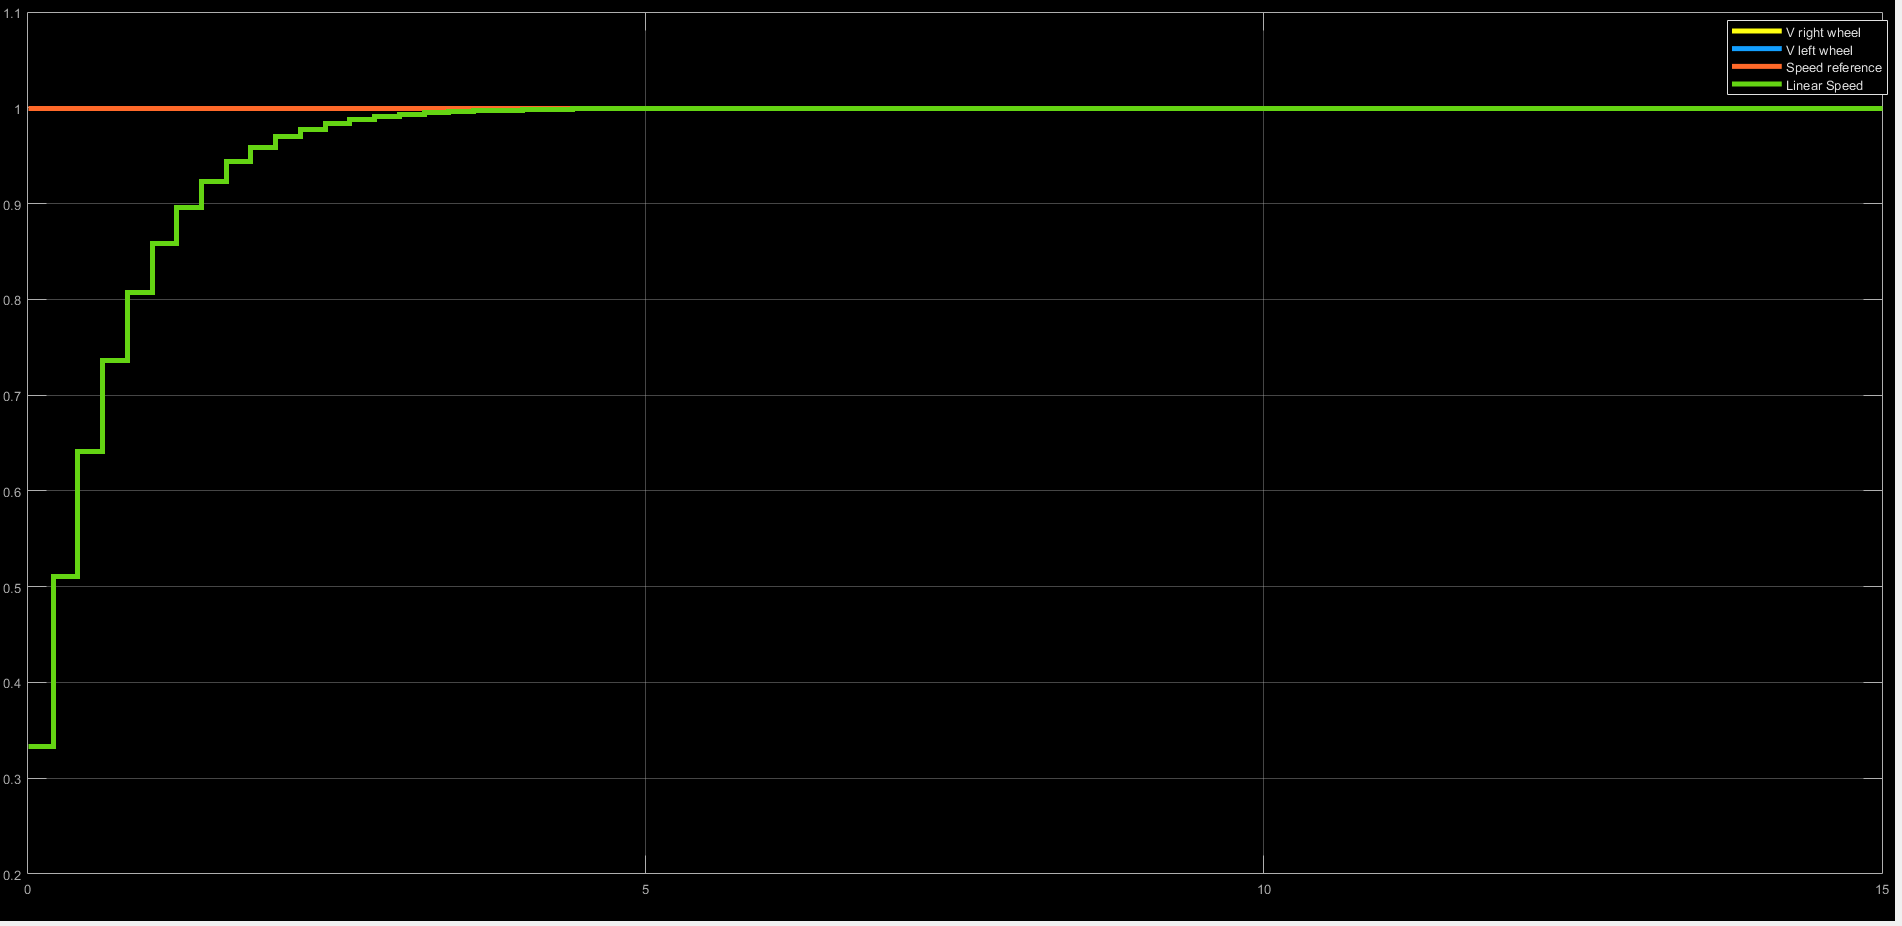
\includegraphics[width=1.0\textwidth]{./img/pid052.png}
\caption {\label{fig:pid1 - p05i2}Kp=0.5, Ki=2}
\end{figure}
As the Kp value was not changed, the initial linear speed value remains the same. As for the time it takes the car to reach steady state, it was reduced to 3 seconds due to the increase of the Ki parameter.\\
In ideal conditions, the aim would be for the car to reach the desired speed
instantly, but due to the real limitations, such as wheel sliding, 3 seconds is
a a safe value.
%
\subsubsection{Sample time determination}
In order to choose the sample time, one needs to take in consideration that with the decrease of the sample time, the processing overhead will increase and with the increase of the sample time, the system response will have abrupt changes affecting the performance of the car. So, in order to accommodate both necessities, the sample time will be set to 50ms.
%\newpage
\subsubsection{System response}
Having determined the parameters of the controller, the next step is to simulate the response of the system.
In order to predict the behavior of the car to a linear speed reference and angle of tilt (teta), some simulations were necessary. The output of the simulation is the plot of the linear speed of the car, the linear speed of both wheels (left and right) and the position of the car.
In order to plot the position of the car the Cartesian referential is used.\\
For the first simulation, the parameters were: Speed reference= 1m/s and teta=0 rad.\\
\begin{figure}[!h]
\centering
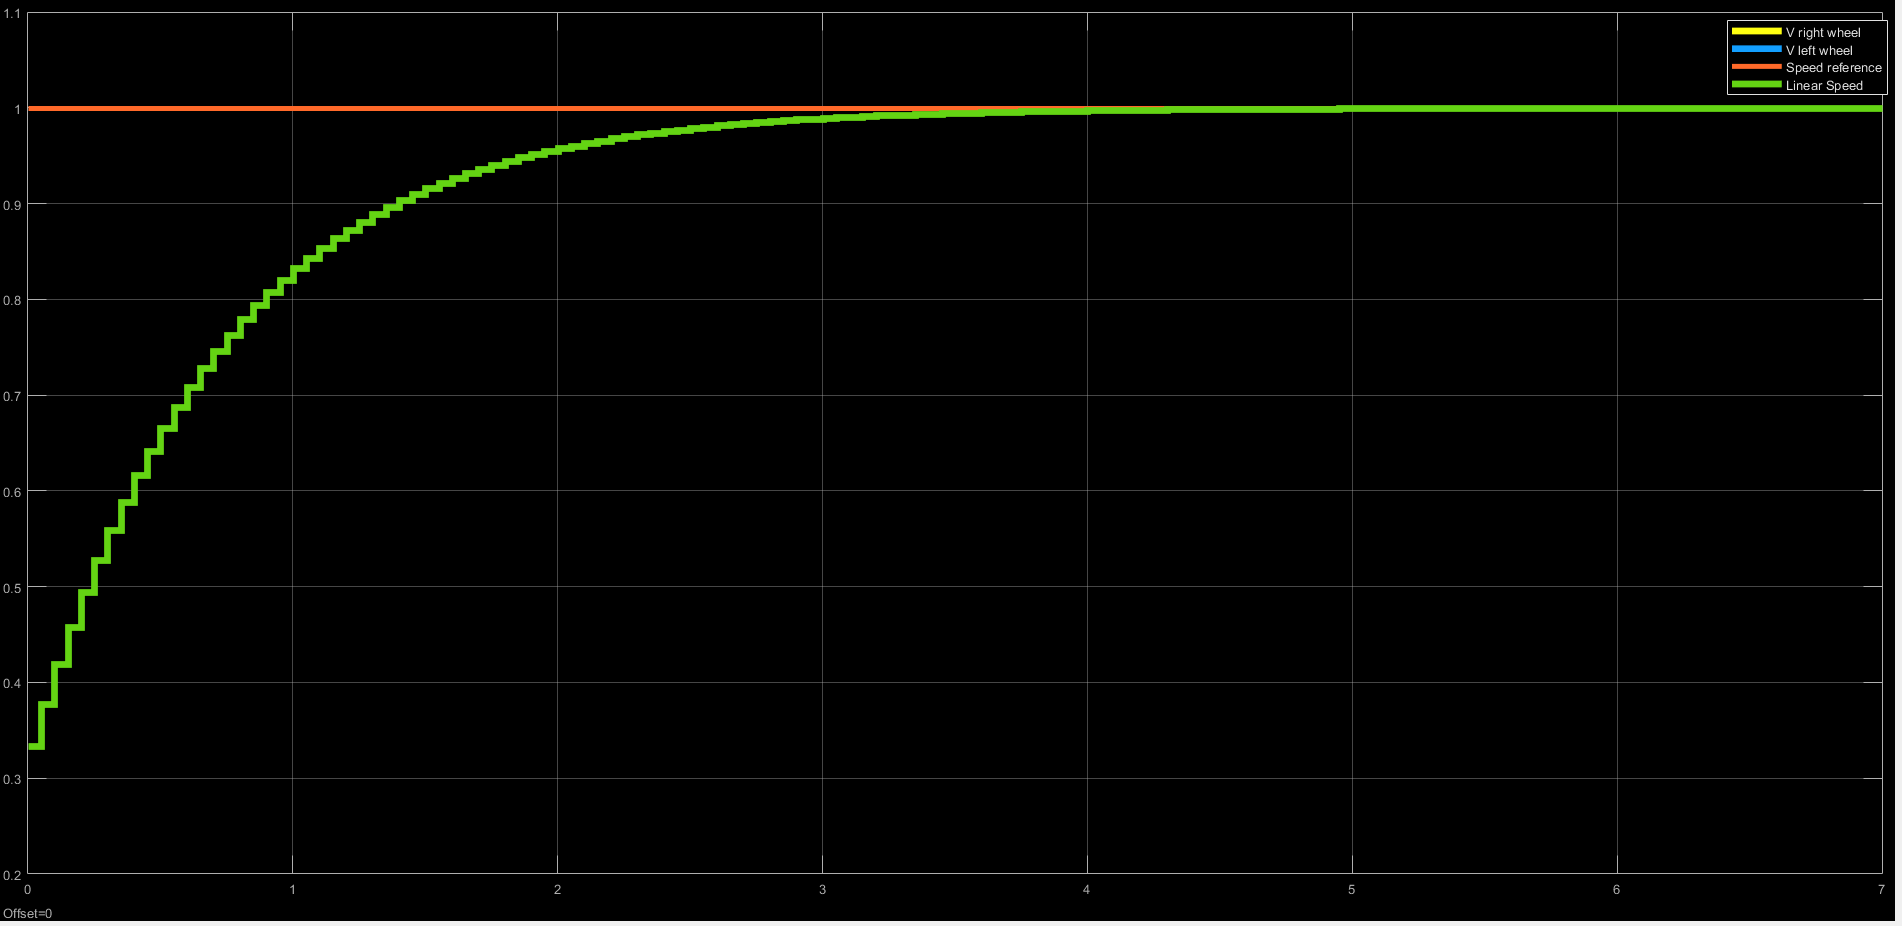
\includegraphics[width=1.0\textwidth]{./img/vel10.png}
\caption {\label{fig:sim1 - vel}Linear speed v=1m/s, teta=0rad}
\end{figure}
 As expected, the car linear velocity reached 1m/s. The angle of tilt is equal to 0 which means the car will be moving in a straight line, and as such, both wheels will are moving at the same speed of the car.\\
\newpage
\begin{figure}[!h]
\centering
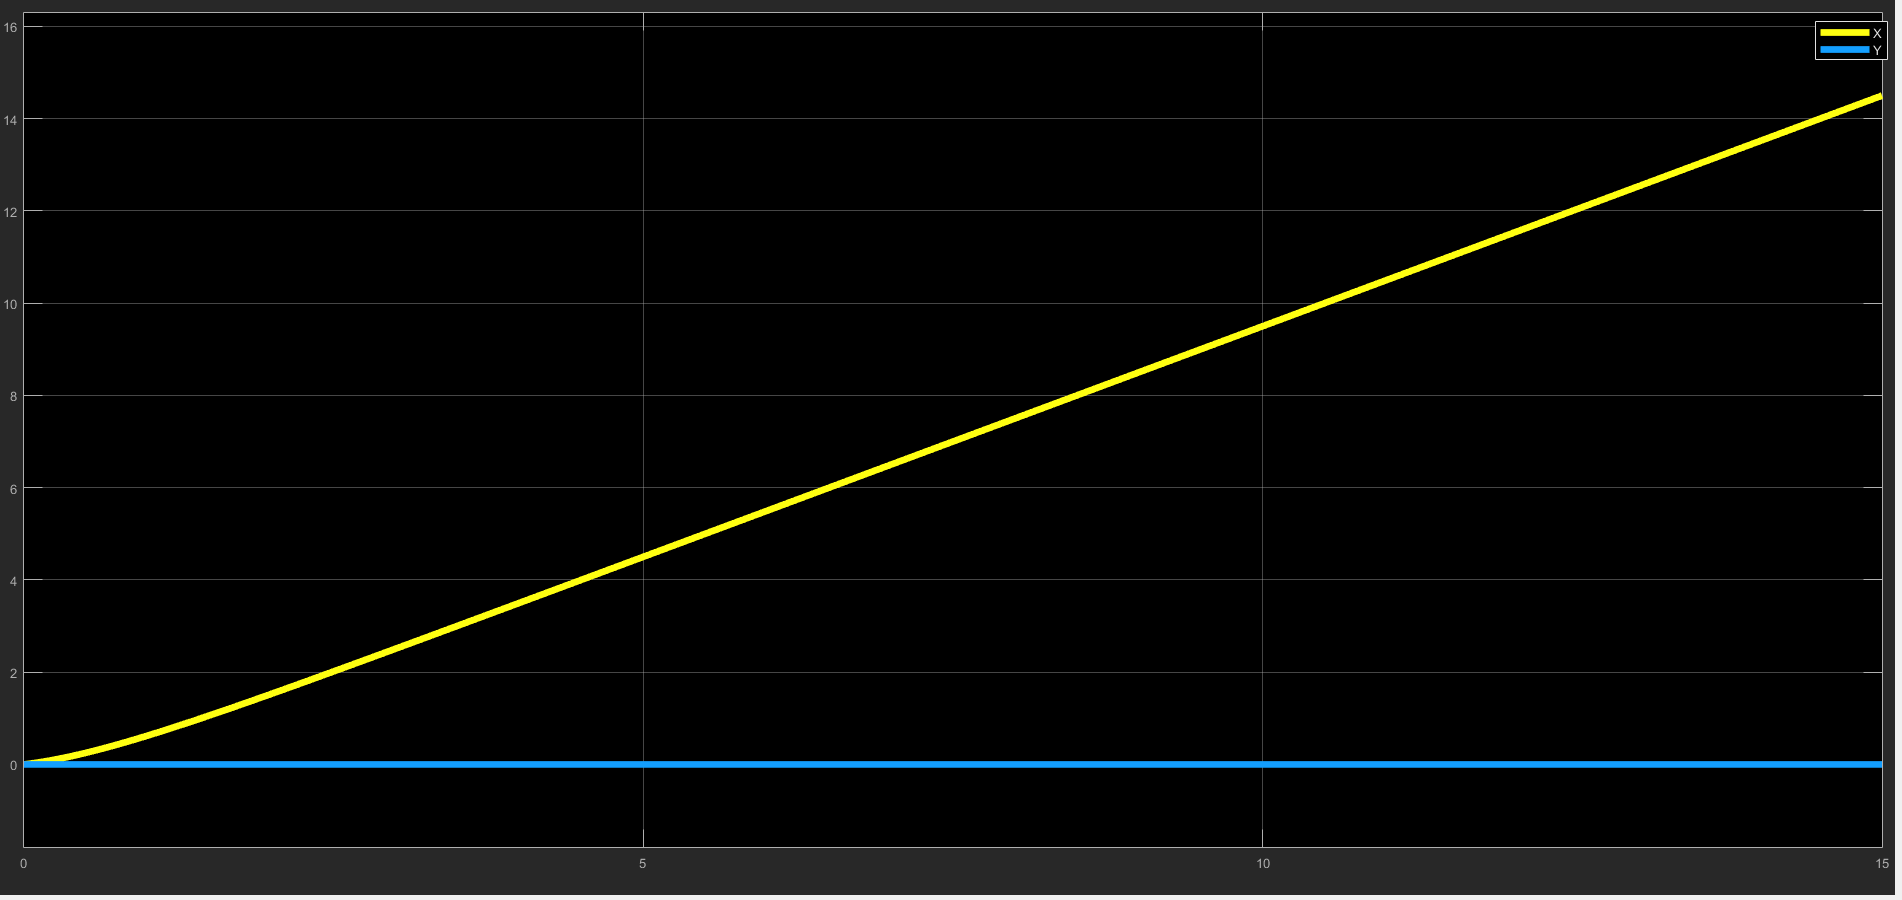
\includegraphics[width=1.0\textwidth]{./img/xy10.png}
\caption {\label{fig:sim1 - pos}Car position v=1m/s, teta=0rad}
\end{figure}
As the teta is equal to 0 rad, only 1 coordinate of the car is moving, as the figure \ref{fig:sim1 - pos} demonstrates. The x coordinate is equal to 0 the entire simulation time, and the y coordinate is increasing with a linear scope equal to the linear velocity of the car. This implies that the car is indeed moving in a straight line.\\
\newpage
Changing the teta to 0.1 rad to simulate constant tilt of the smart phone to the right, and maintaining the value of the speed reference in 1 m/s :\
\begin{figure}[!h]
\centering
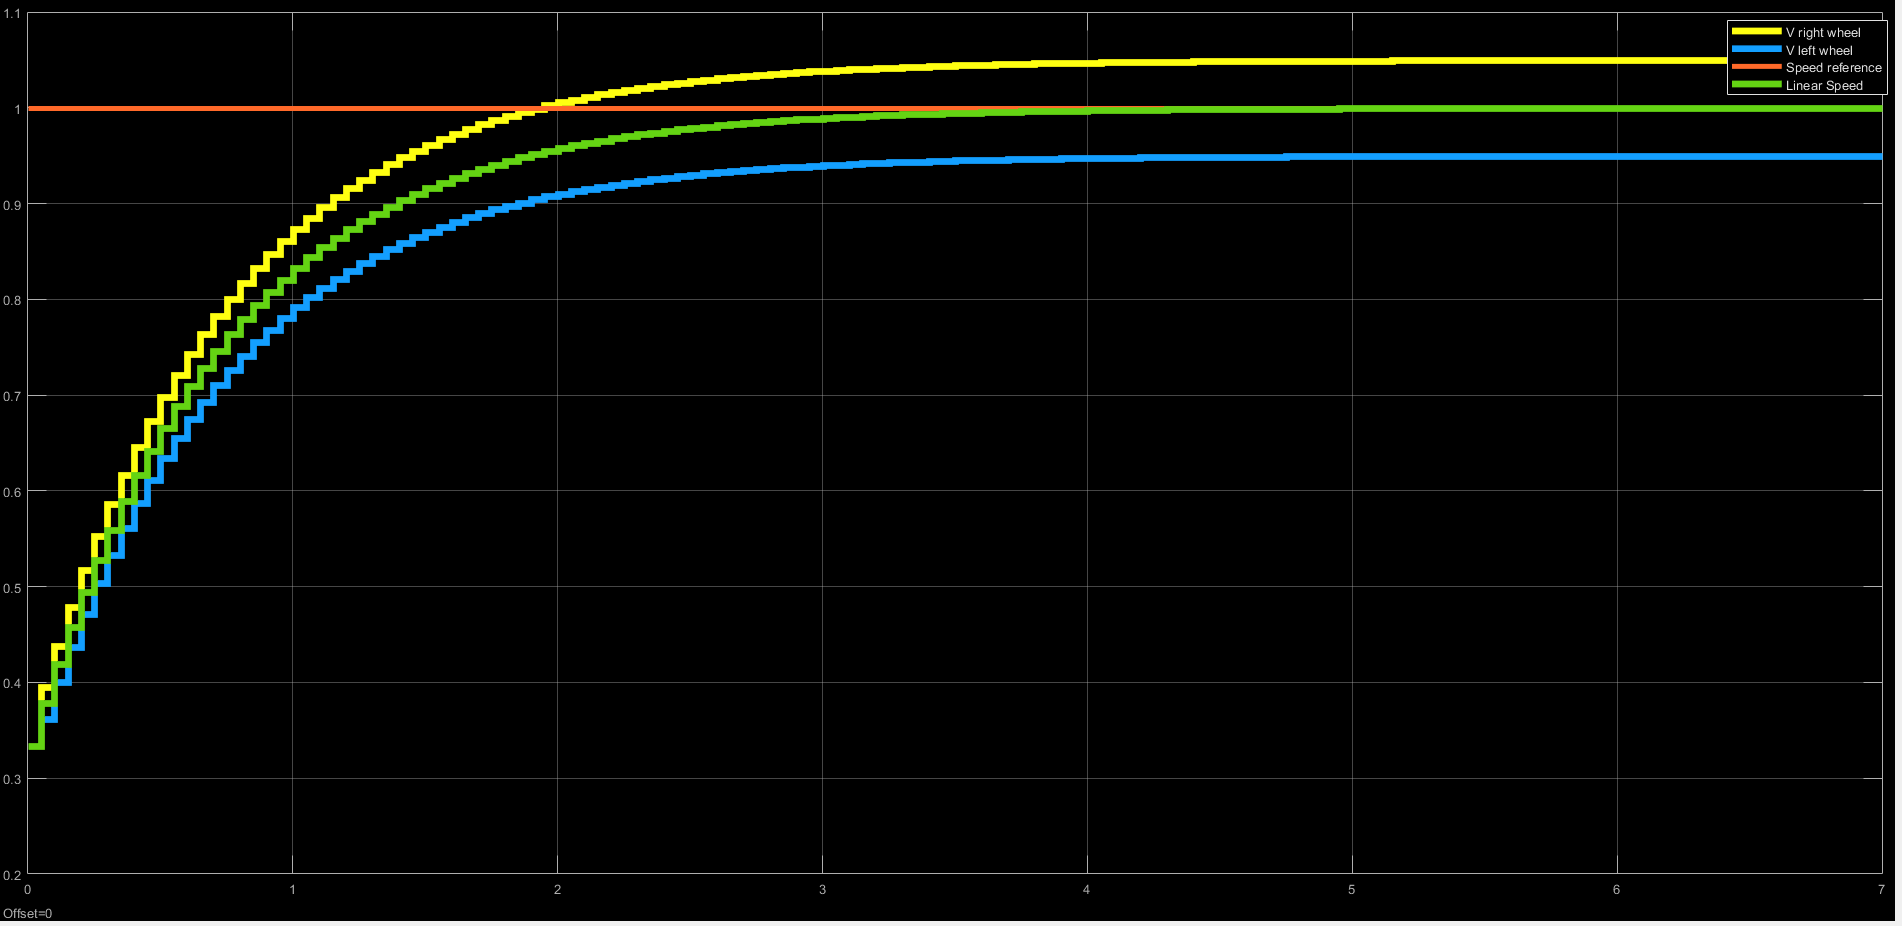
\includegraphics[width=1.0\textwidth]{./img/vel101.png}
\caption {\label{fig:sim2 - vel}Linear speed v=1m/s, teta=0.1rad}
\end{figure}
In this simulation it can be observed that having a angle of tilt not equal to 0, causes the left and right wheels to have different velocities, in order to make the car turn. Running more simulations with different values of teta, the outcome shows that the bigger the module of the value of teta, the bigger the difference between the linear velocities of the wheels.
\begin{figure}[!ht]
\centering
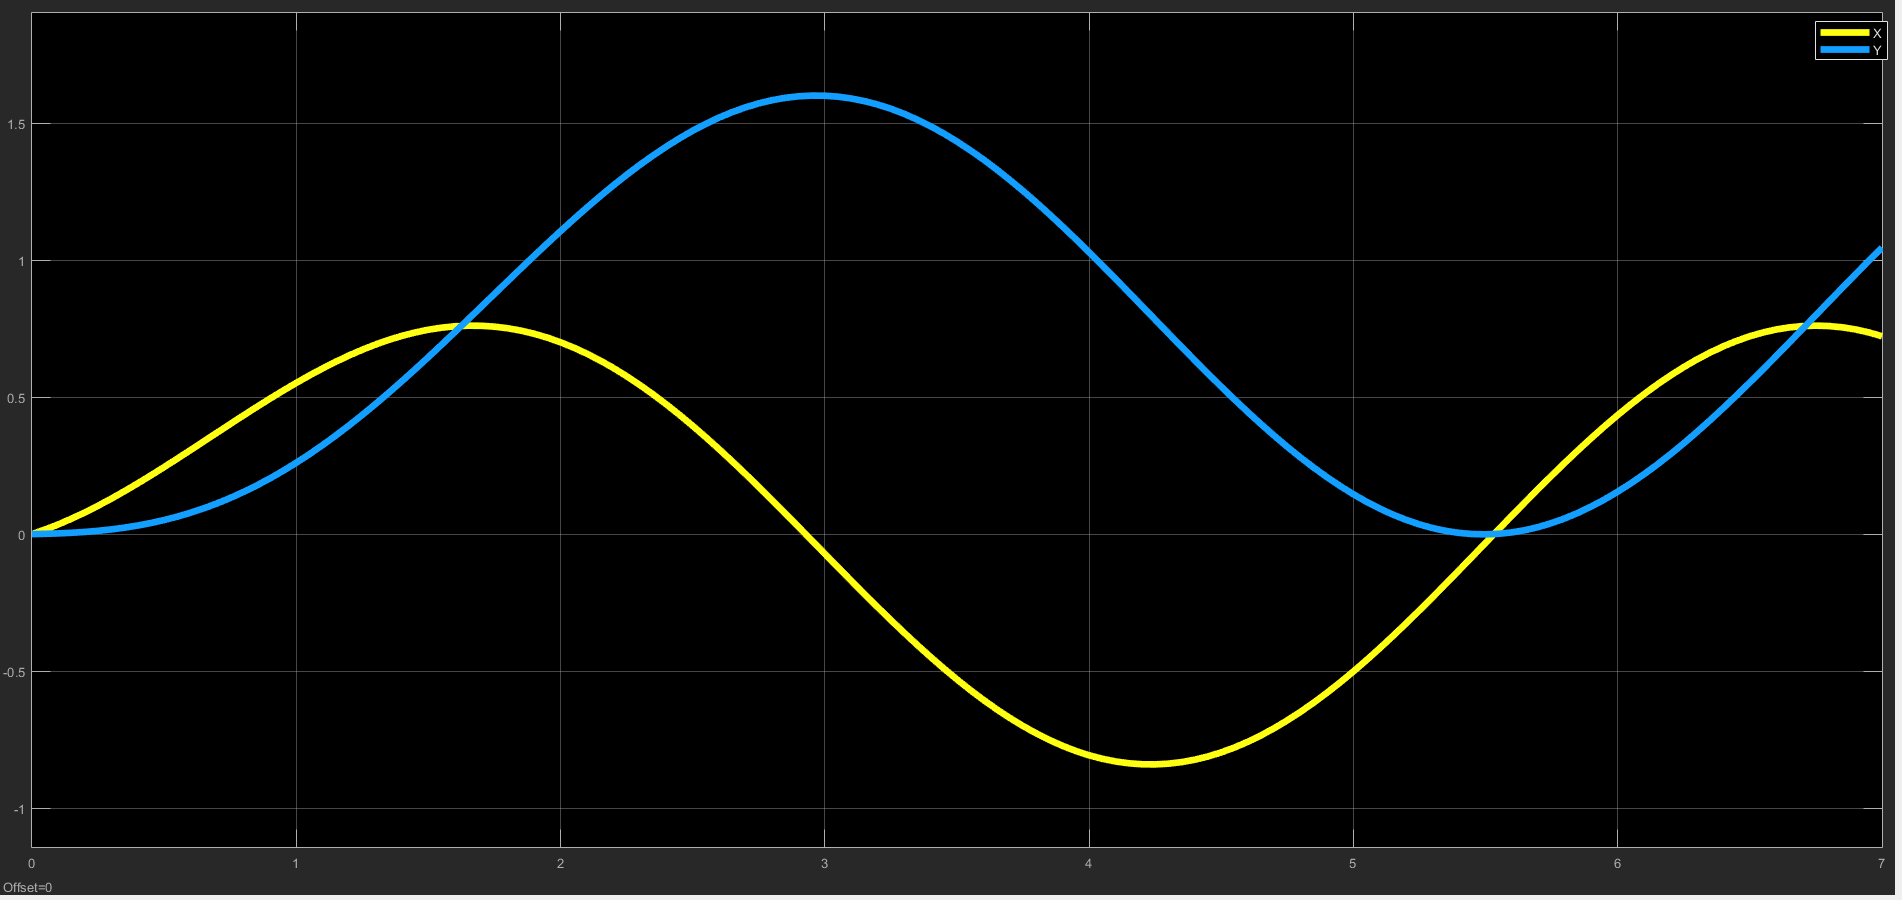
\includegraphics[width=1.0\textwidth]{./img/xy101.png}
\caption {\label{fig:sim2 - pos}Linear speed v=1m/s, teta=0.1rad}
\end{figure}
With this figure \ref{fig:sim2 - pos} it is possible to observe that both the
position of x and y of the car change with time. With a constant angle of tilt,
the car will turn constantly in the same direction, eventually making a 360
degrees turn and as the car as small dimensions, it takes a very small time for
it to do so, which is what is observed is this simulation.
%%% Local Variables:
%%% mode: latex
%%% TeX-master: "../../../dissertation"
%%% End:

\subsubsection{Obstacle Avoidance Through Odometric Sensors}
Wireless communication between devices is always prospect to errors and obstructions, as such a way had to be devised so that the rover will function safely when communications fail whilst also avoiding a significant decline in the system's life expectancy.\\In order to achieve this, several odometric sensors will be placed on the rover, covering the \ang{360} radius, and whenever it judges an obstacle is too close (through the feedback of the sensors) it will not follow commands that would force it to get any closer to said obstacle.\\The implementation of an autonomous obstacle avoidance algorithm was considered, however implementing such an algorithm would, in the best scenario, remove control from the user and, in the worst scenario, enter into direct conflict with the latter. Therefore, since neither of the aforementioned scenarios was in the best interests of either the system or the user, it was opted to simply force the system to stop if a command would take it too close to an obstacle and to not allow it to move towards it any further.
\subsubsection{Obstacle Avoidance Simulations}
In order to plot the rover's path on a 2D diagram, the \textit{Mobile Robotics Simulation Toolbox}, made available by MATLAB, will be used. A series of waypoints  (these will simulate the user's commands) will be placed on a 2D map with borders, the latter of which will be used as obstacles. The waypoints shall direct the rover towards one of the borders in a turn and a straight line. Ideally the rover will stop before reaching the obstacle whilst also keeping enough space to turn away from it.\\
\\
The initial position of the rover shall be at coordinates (1,1) and an angle of 0 rads, as depicted in Fig.~\ref{fig:iniState}. 
From this standpoint, two simulations will be considered: a straight line that will require a $\frac{\pi}{2}$ rads turn upward (this turn serves to test the algorithm, to make sure it does not stop changes in direction whilst away from obstacles) and head straight towards one of the walls of the map;
and a second simulation, involving a turn towards a wall. In order either simulation to be a success the rover must stop before crashing against the wall with enough space to steer away from the obstacle.

\begin{figure}[!htbp]
\centering
       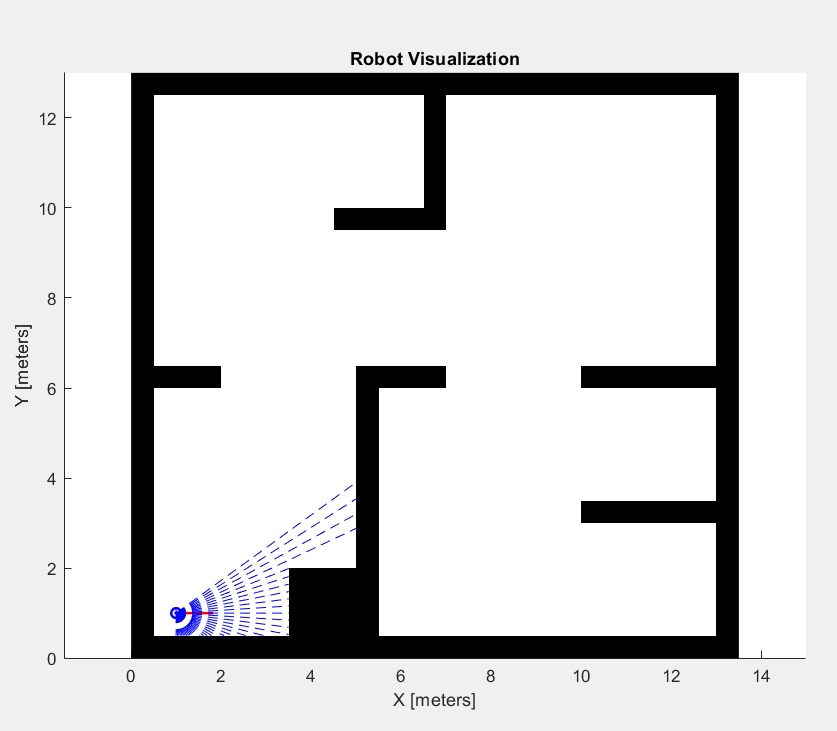
\includegraphics[page=1,width=0.55\textwidth]{img/startState.png} 
\caption{Initial State of simulation}
\label{fig:iniState}
\end{figure}

Firstly it must turn towards the wall, Fig~\ref{fig:sim1Turn}.
\begin{figure}[!htbp]
\centering
       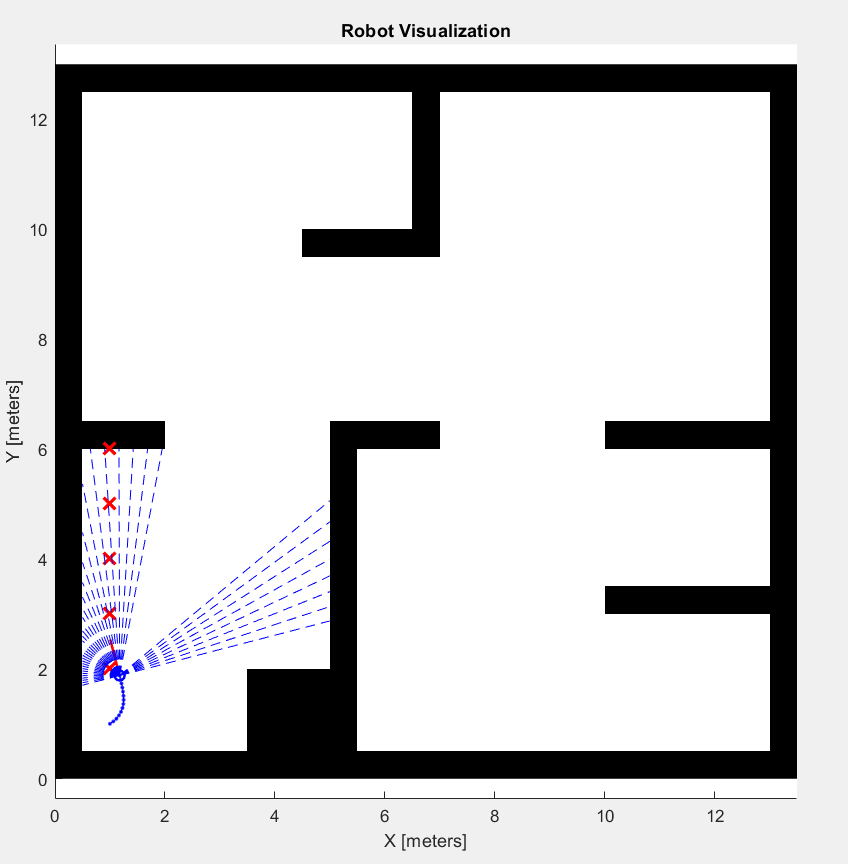
\includegraphics[page=1,width=0.55\textwidth]{img/line2.png} 
\caption{After Rover Turns Towards Wall}
\label{fig:sim1Turn}
\end{figure}

Afterwards it must head in a straight line and stop before the obstacle, Fig~\ref{fig:sim2Line}

\begin{figure}[!htbp]
\centering
       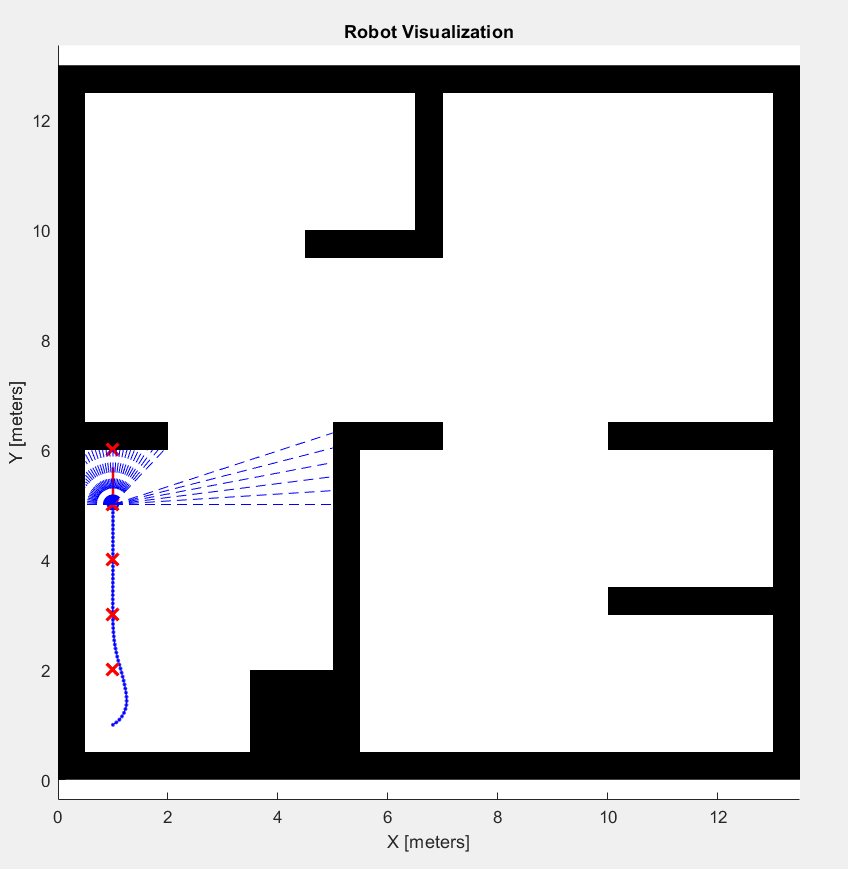
\includegraphics[page=1,width=0.55\textwidth]{img/line3.png} 
\caption{Rover Stopped Before Reaching Wall}
\label{fig:sim2Line}
\end{figure}

In the second simulation, which shall start, once again from the initial position depicted in Fig.~\ref{fig:iniState}, the rover must turn towards a path that avoids the right wall, Fig.~\ref{fig:sim2Line} and afterwards turn again and stop before reaching the wall with enough space to turn away from the latter, Fig.~\ref{fig:sim3Line}.

\begin{figure}[!htbp]
\centering
       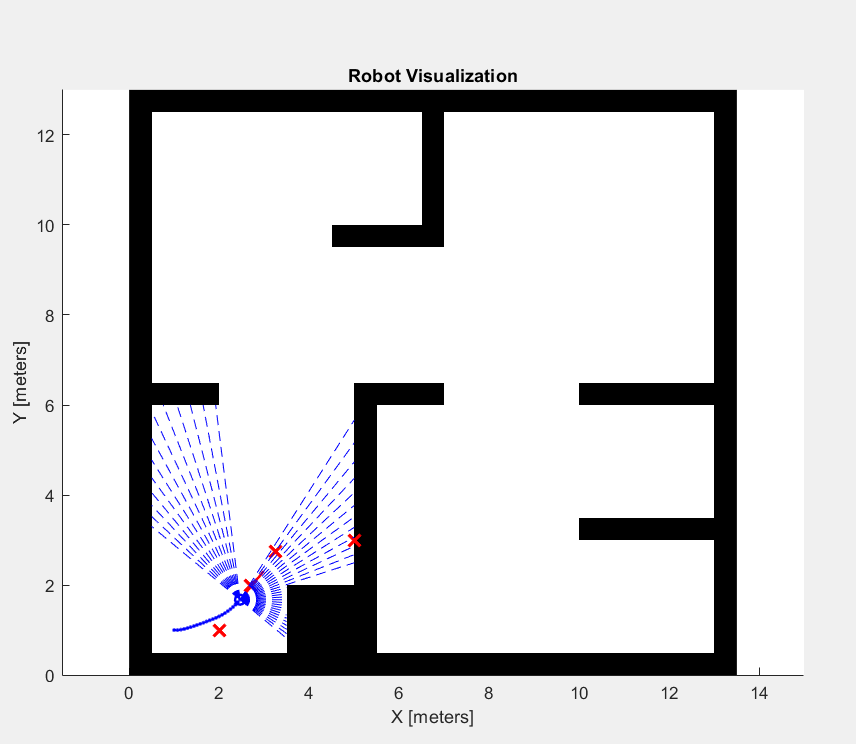
\includegraphics[page=1,width=0.6\textwidth]{img/turn2.png} 
\caption{Rover Starts the Turn}
\label{fig:sim2Line}
\end{figure}

\begin{figure}[!htbp]
\centering
       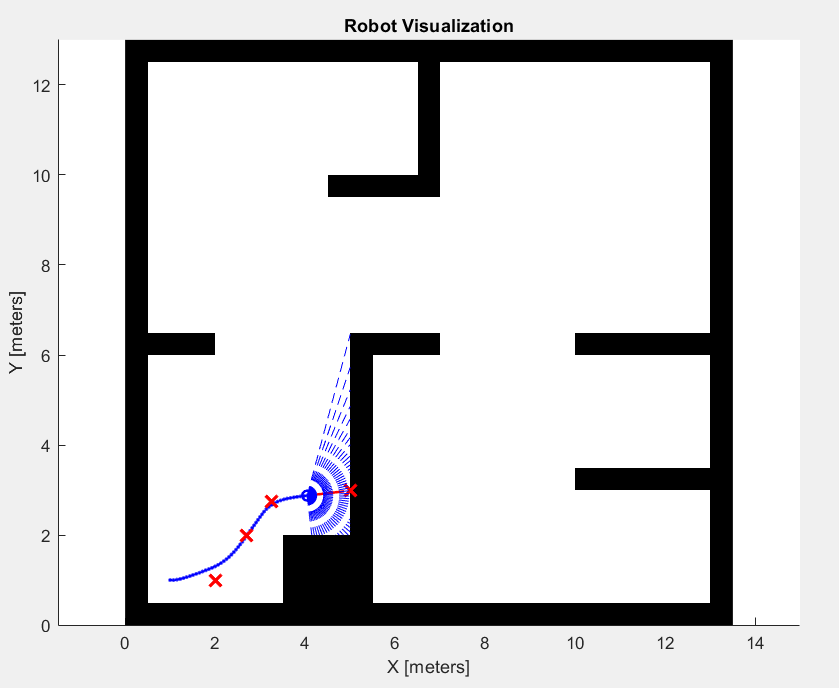
\includegraphics[page=1,width=0.6\textwidth]{img/turn3.png} 
\caption{Rover Turned and Stopped Before Reaching Wall}
\label{fig:sim3Line}
\end{figure}
\newpage

\subsubsection{Odometric Sensor} 
For the obstacle avoidance, several of \href{https://www.botnroll.com/pt/infravermelhos/158-sen-00242.html}{GP2Y0A21YK Infrared Sensors} (Fig~\ref{fig:sensor}) will be placed on the rover, since it has an allowable field angle of up to \ang{40}, this would mean at least 9 sensors would be required to cover \ang{360}, this is assuming that they are placed in such a way that there is no overlap, however since any sort of "blind spot" will place the rover in jeopardy, some overlap is desired. Considering the rover's dimensions, it is unlikely that 9 sensors can be placed upon it with enough overlap to completely cover the \ang{360}, therefore it is likely that a few more will have to placed to guarantee safety of the rover.

\begin{figure}[!htbp]
\centering
       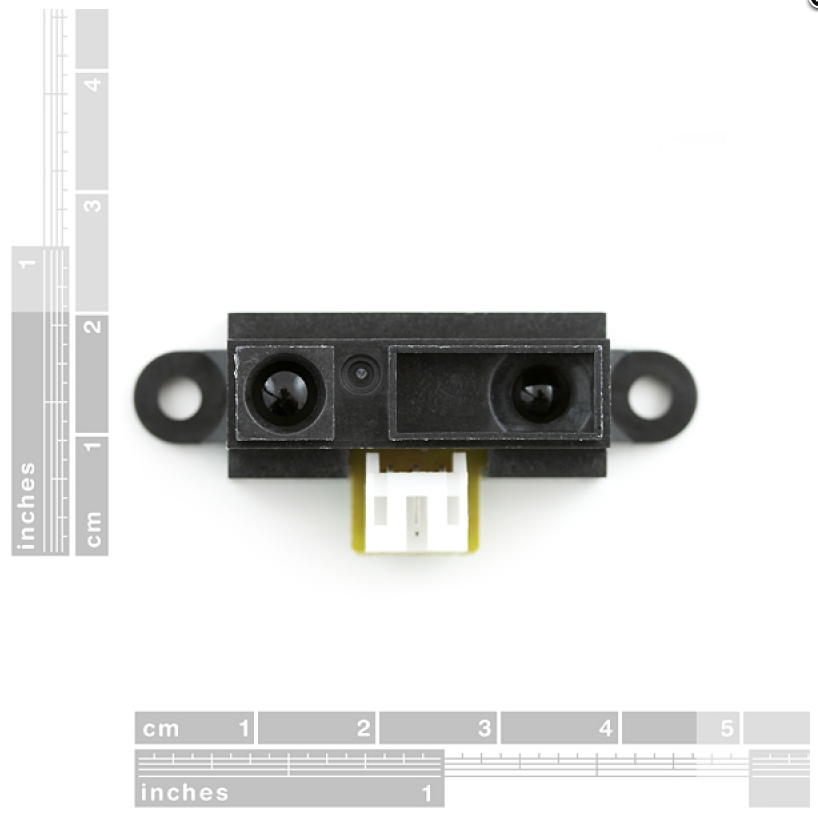
\includegraphics[page=1,width=0.35\textwidth]{img/sensor.png} 
\caption{Odometric Infrared Sensor GP2Y0A21YK}
\label{fig:sensor}
\end{figure}
%
\subsection{System design}%
\label{sec:navigation-system-design}
Tackling the objectives laid out in \cref{sec:navig-virt-subsyst-design} requires an organized and well thought-out plan of work because there are a lot of smaller systems at play that need to work cohesively and synchronously. 




%///////////////////////// # Separation into packages //////////////////////////

The best way to achieve a good plan is by first separating the problem into packages, and in each package have subpackages, each with a collection of modules dedicated to serve a collective purpose in the data treatment and organization chain. 

The system is divided into such packages as follows:

\begin{figure}[H]
	\centering
	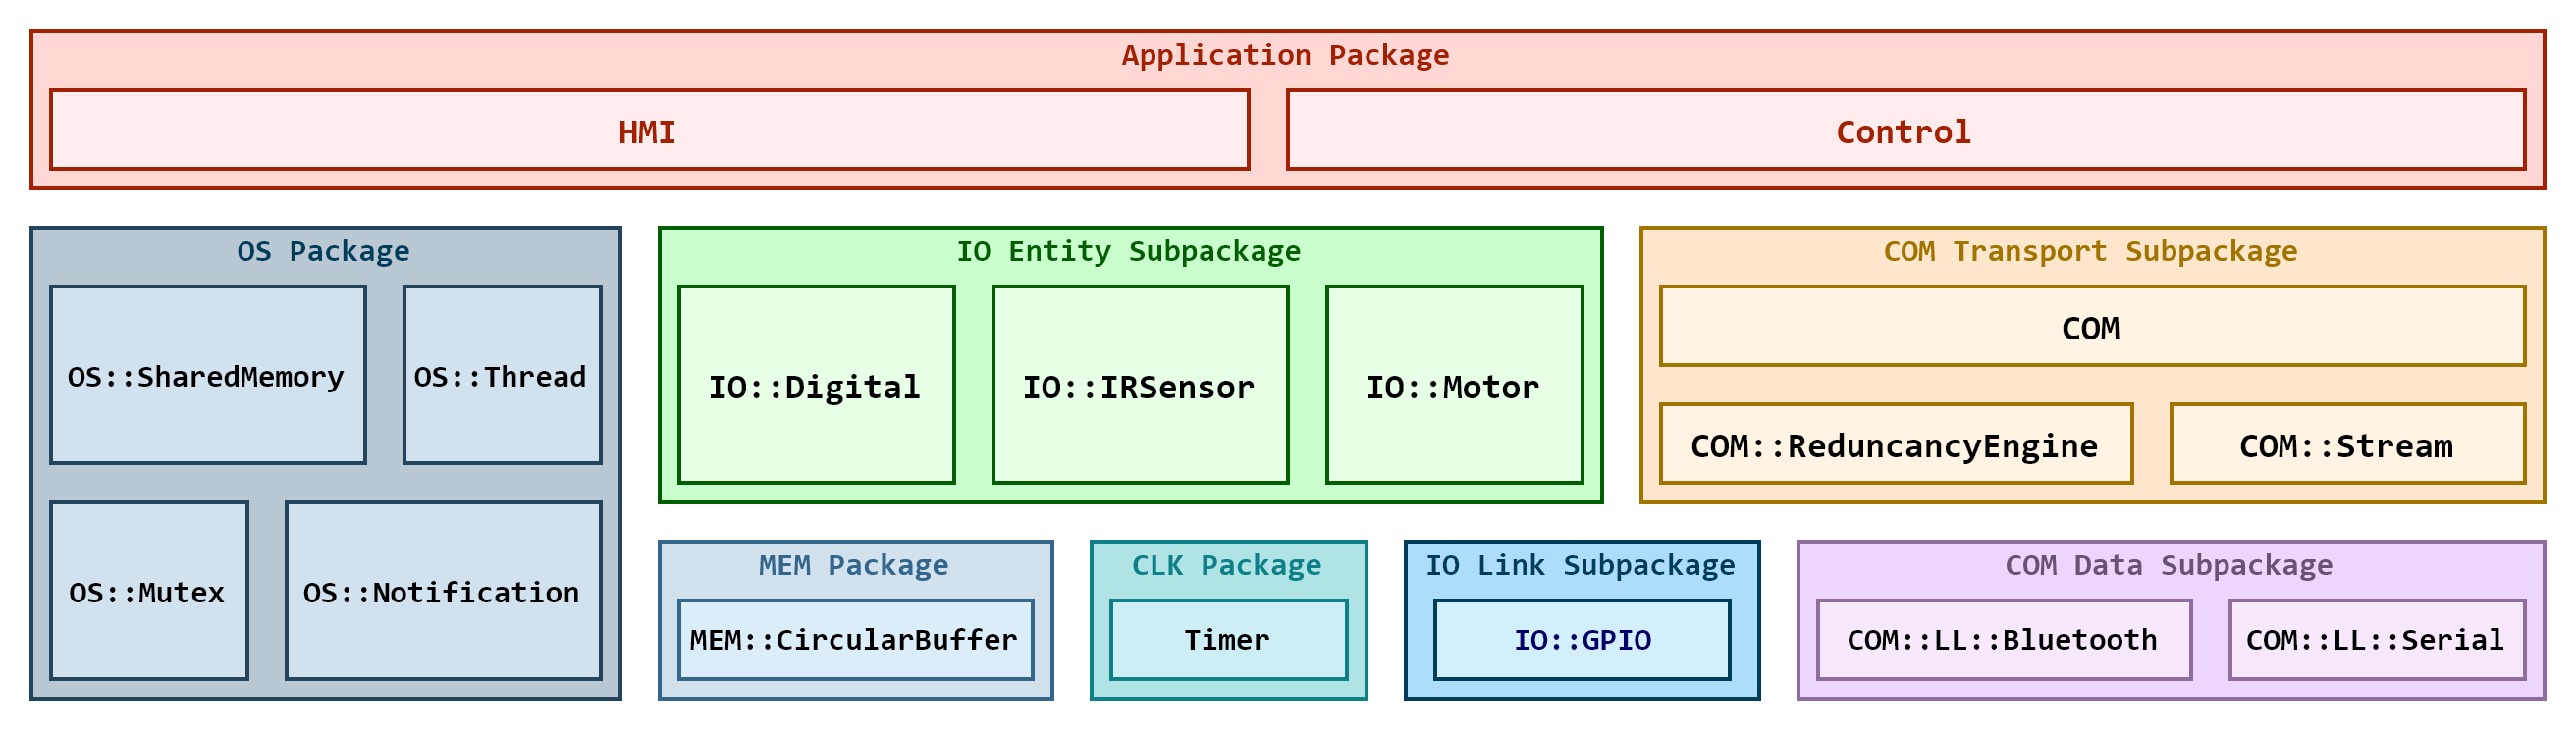
\includegraphics[width=1.0\textwidth]{./img/full-stack-overview.png}
	\caption {Full Stack Overview}
	\label{fig:full-stack-overview}
	\end{figure}
	


%////////////////////////// # Separation into layers ///////////////////////////

Each subpackage also belongs to a certain layer of software, characterized not by the resources it is associated to but by how close the modules within it are to the hardware. Futhermore, the packages should be distributed between layers in such a way that one seldomly need to use another that doesn't belong to the same layer or the layer directly below. 


These layers are, from the bottom to the top:
\begin{itemize}
	\item The High-level Hardware Abstraction Layer, which consists of the \textbf{OS} (partly), \textbf{MEM}, \textbf{CLK}, \textbf{IO Link} and \textbf{COM Data} packages/subpackages. Modules within this layer are responsible for the lower-level interaction with the system's resources so they are made to be thread-safe. Their implementation is platform-dependent and their interface is platform-agnostic. The main goal for this layer of software is to standardize the hardware, making for clean, maintainable and easily portable code. 
	\item The High-level Software Abstraction Layer, consisting of the \textbf{OS} (partly), \textbf{IO Entity} and \textbf{COM Transport} packages. The modules within these packages should serve as an interface with the lower level layer, creating a more intuitive interaction process and mechanisms for processing information asynchronously. This way, when other modules make use of those interfaces, the information is already parsed and ready to be retrieved.\\
	Modules in the layers above ara also highly dependent on both abstraction layers to carry out their tasks in time so the ones in this layer should provide robust mechanisms for exception-handling and timing. 
	\item The Main Application Layer, comprised only of the \textbf{APP} package, where the core functionality lies. As stated earlier, modules in this layer are protected from having to access to most lower-level layers but can use those modules and must use when no other abstraction is provided.
\end{itemize}


%//////////////////////////////// Static model /////////////////////////////////
\subsubsection{Static Model: Package diagram}

\begin{figure}[H]
	\centering
	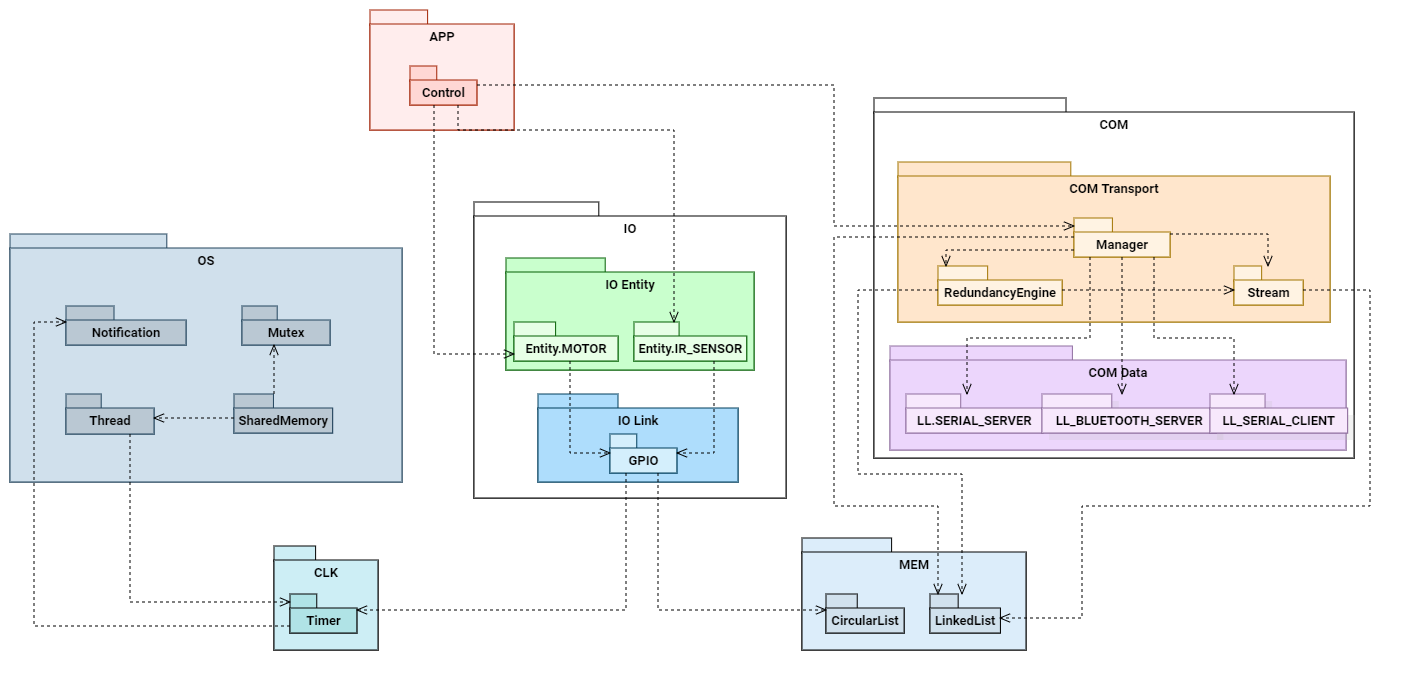
\includegraphics[width=0.8\textwidth]{./img/navig-package-diagram.png}
	\caption {Navigation subsystem package diagram}
	\label{fig:navig-package-diagram}
	\end{figure}



\subsubsection{Static Model: Class diagram}


\begin{figure}[H]
	\centering
	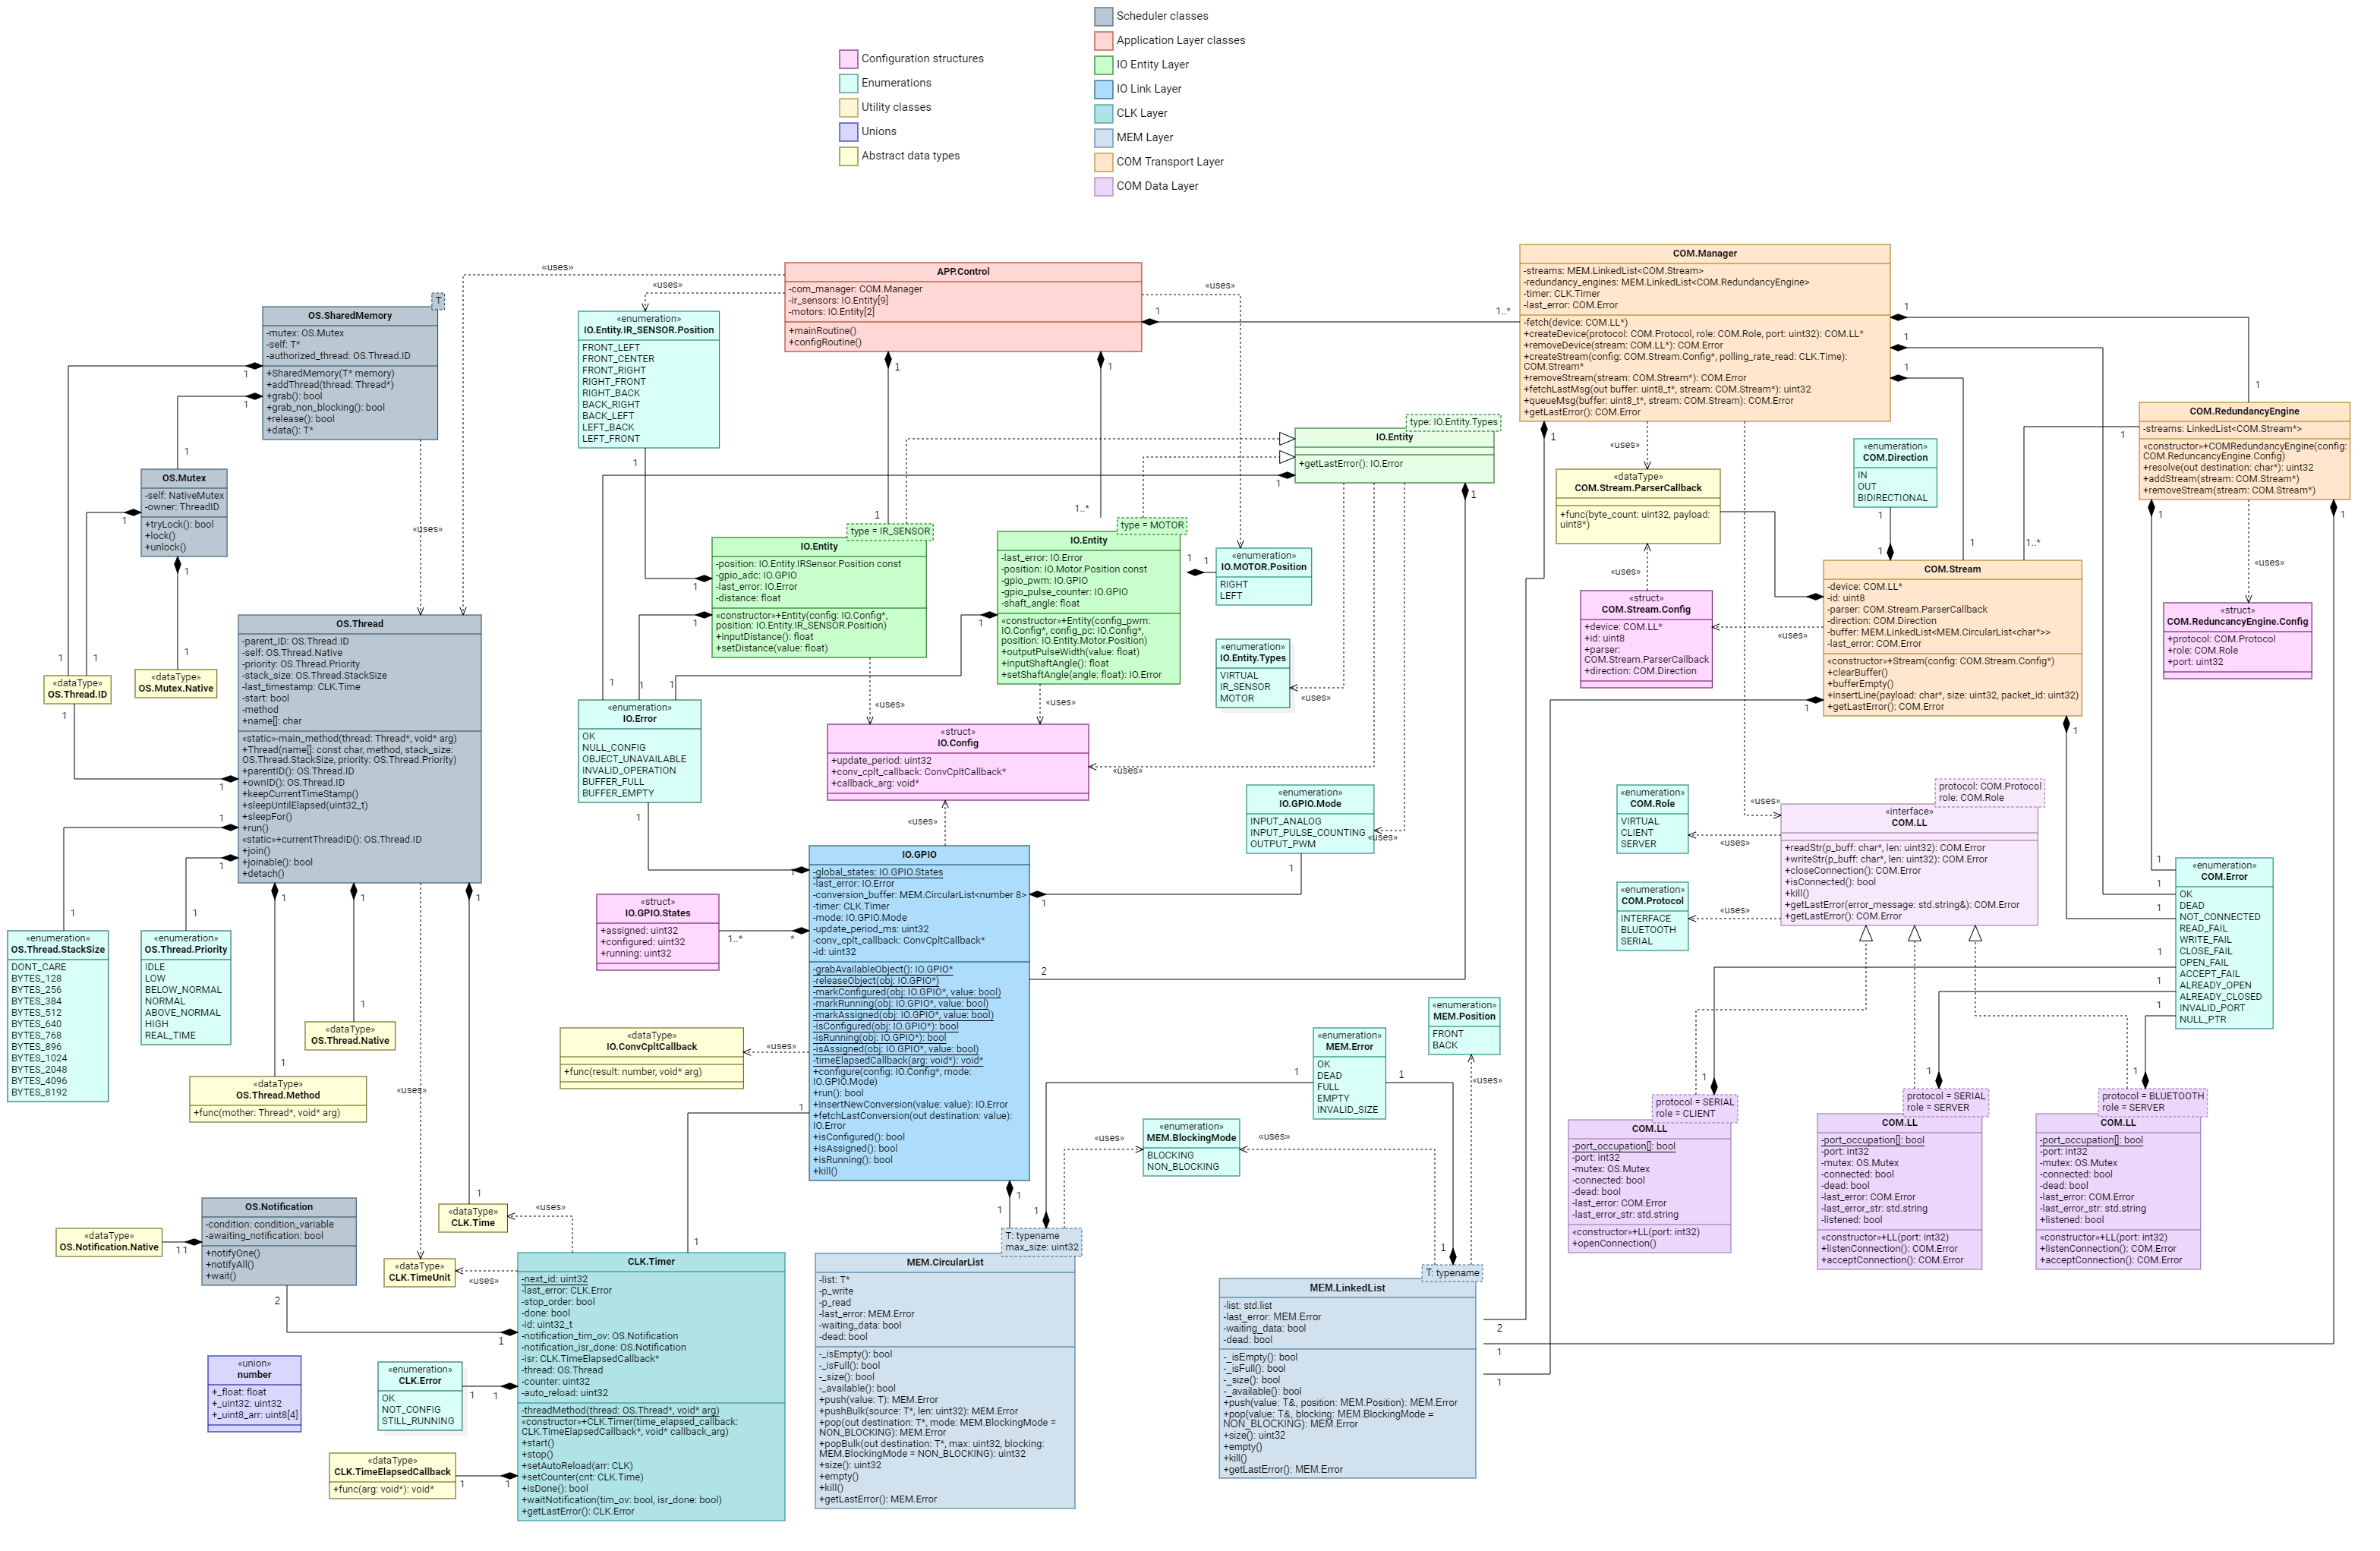
\includegraphics[width=\textwidth]{./img/navig-class-diagram.png}
	\caption {Navigation subsystem class diagram (augmented in Appendix \ref{fig:navig-class-diagram-augmented})}
	\label{fig:navig-class-diagram}
	\end{figure}



%//////////////////////////////// # IO Package /////////////////////////////////
\subsubsection{IO: Input/Output Package}
\label{sec:io-package}
The \textbf{IO} package is comprised of the \textbf{IO Entity} and \textbf{IO Link} subpackages. The modules within these subpackages are the parts of the hardware abstraction layers responsible for standardizing the General Purpose Input/Output resources of the machine.

The \textbf{IO Link} subpackage is the interface provides the most generic yet complete package for interacting with the machine. Its only module \textbf{IO::GPIO} provides such functionality as automatic resource assignment upon creation, automatic buffering of read and output values and the option of executing a specific piece of code when a conversion is completed for better effort distribution between layers.

\begin{figure}[H]
	\centering
	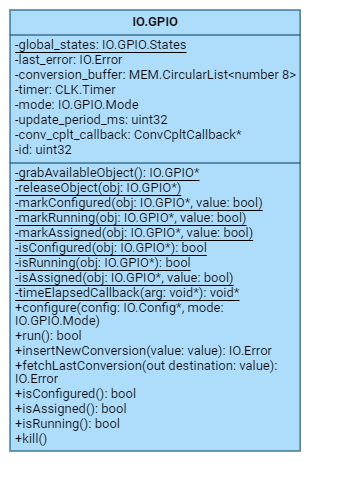
\includegraphics[width=0.38\textwidth]{./img/navig-class-gpio.png}
	\caption {IO::GPIO interface and members}
	\label{fig:navig-class-gpio}
	\end{figure}


The \textbf{IO::Entity} module from the \textbf{IO Entity} subpackage serves for specialization of functionality present in \textbf{IO Link} to serve a certain purpose attached to a physical meaning. This means it also extends the aforementioned callback mechanisms from \textbf{IO::GPIO} for automatic calculation of real-world values based on the measurements taken or otherwise that can be adapted and tailored further to serve the purpose of the specific application. Both provide a modest interface for storing important values calculated in the context of a \texttt{IO::ConversionCpltCallback} and a way to retrieve them.\\

Its \texttt{MOTOR} specialization uses an instance of \textbf{IO::GPIO} as an \texttt{INPUT\_PULSE\_COUNTING} to be able to count the number of pulses from the motor's encoder and output and one as an \texttt{OUTPUT\_PWM} to be able to output a pulse width modulated signal with a duty-cycle $D$ such that 
$$
V_{out average} = \frac{D\times V_{max}}{100}
$$

The \texttt{IR\_SENSOR} specialization uses an instance of \textbf{IO::GPIO} as an \texttt{INPUT\_ANALOG} for application in IR sensing applications. It provides a way to change the last calculated distance specifically for use in the corresponding callback function and an interface for retrieving that same value.

\begin{figure}[H]
	\centering
	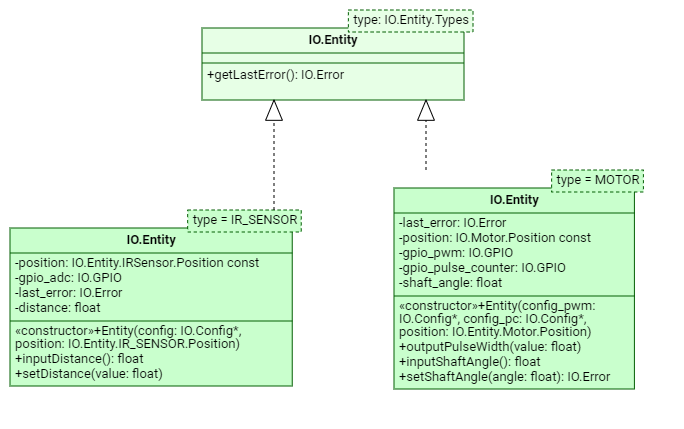
\includegraphics[width=0.65\textwidth]{./img/navig-class-entity.png}
	\caption {IO::Entity interface and specializations' methods and members}
	\label{fig:navig-class-entity}
	\end{figure}



\begin{figure}[H]
	\centering
	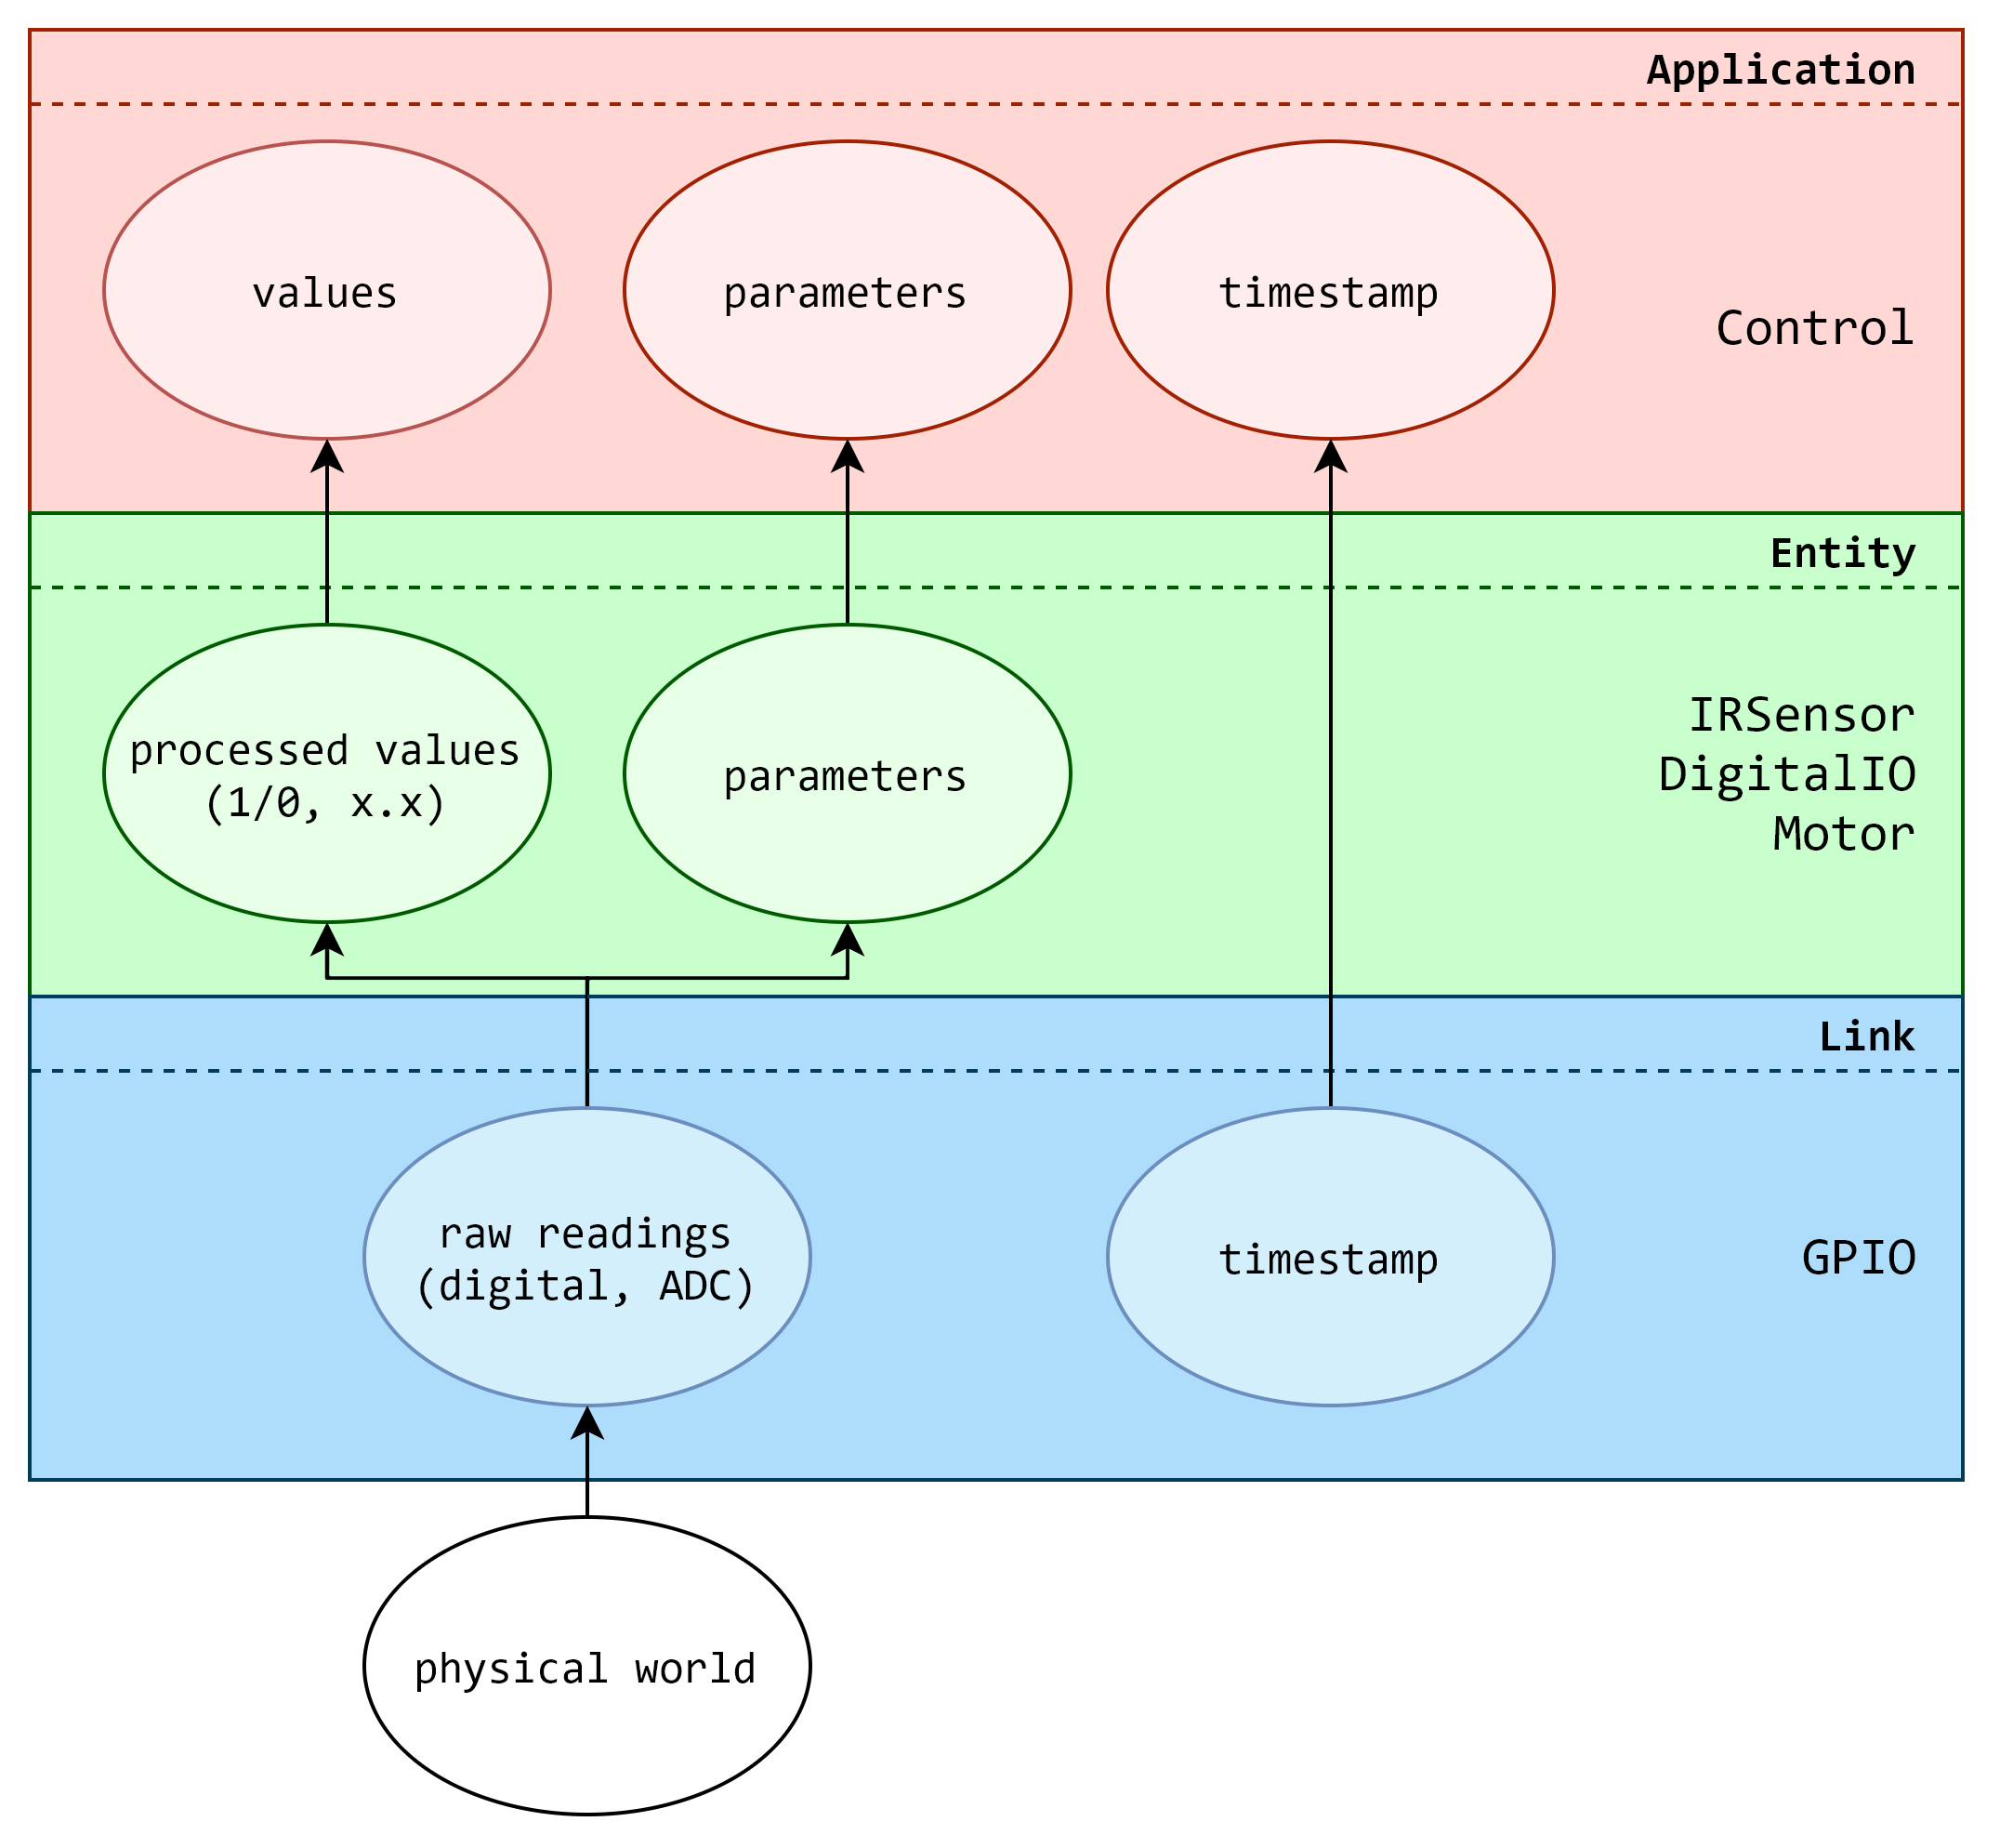
\includegraphics[width=0.5\textwidth]{./img/module-stack-io.png}
	\caption {IO subpackage interaction and information propagation diagram}
	\label{fig:navig-module-stack-io}
	\end{figure}

 

%//////////////////////////////// # COM Package ////////////////////////////////
\subsubsection{COM: Communications Package}

The COM package is the sum of the COM Data and COM Transport subpackages. These  modules are responsible for standardizing the access to the inter-device communication resources of each machine. 


The \textbf{COM Data} subpackage is aimed at providing a platform-agnostic interface for communicating over a serial or Bluetooth connection, while also providing specific functionality for different protocols/roles.
The \textbf{COM Transport} subpackage provides tools for managing multiple simultaneous, redundant, multiprotocol and multi-stream connections as well as automatically parsing of data for usage in time-constrained scenarios.

\begin{figure}[H]
	\centering
	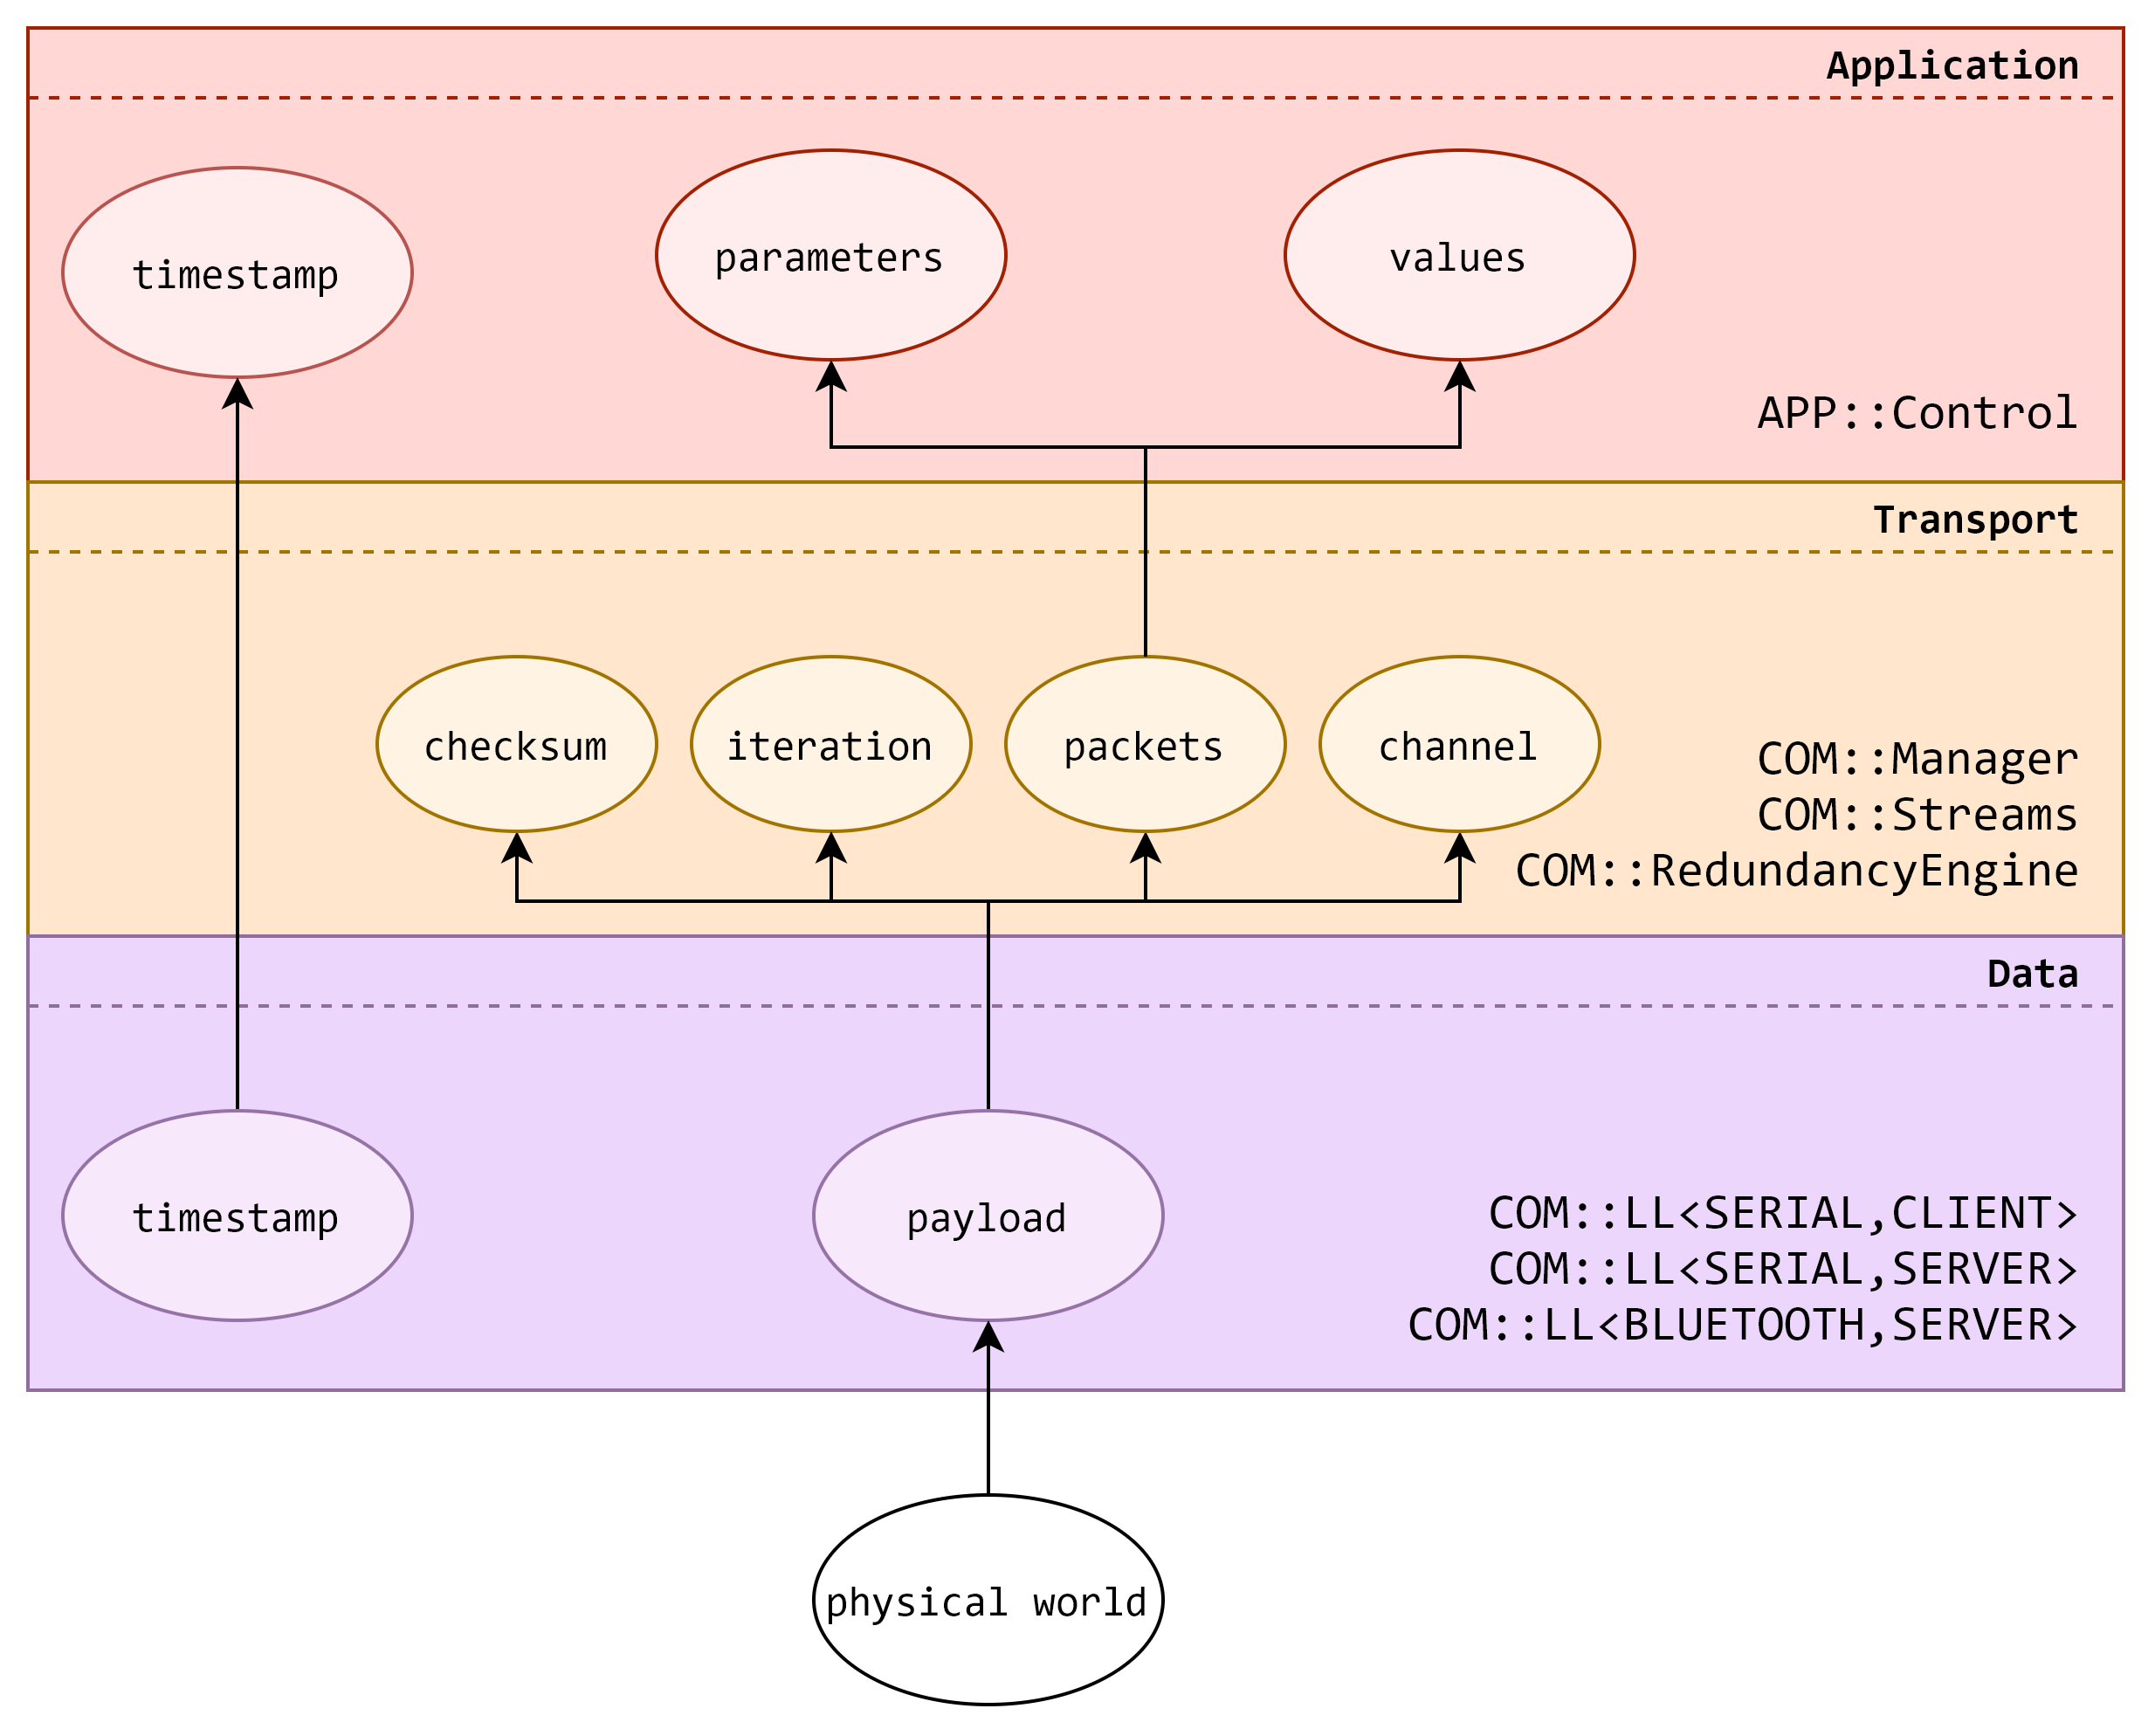
\includegraphics[width=0.5\textwidth]{./img/module-stack-com.png}
	\caption {COM subpackage interaction and information propagation diagram}
	\label{fig:navig-module-stack-com}
	\end{figure}



The \textbf{COM::LL} module makes up the lower layer of the COM package. It should then have very well defined and error-tolerant behaviour and a somewhat familiar interface. With that in mind, it had an error-reporting system that would give feedback over a variery of errors such as invalid ports or non existing connections. It has been envisioned to be capable of connecting devices through serial and bluetooth protocols using a typical client and server socket model.

\begin{figure}[H]
	\centering
	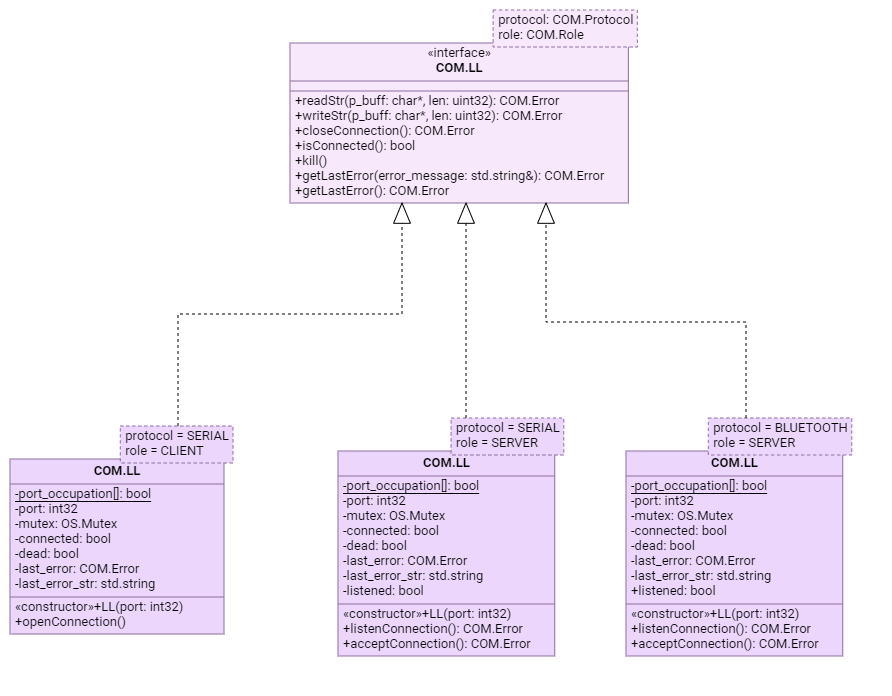
\includegraphics[width=0.8\textwidth]{./img/navig-class-ll.png}
	\caption {COM::LL interface and specializations' methods and members}
	\label{fig:navig-class-ll}
	\end{figure}


The \textbf{COM::Stream} module allows the partitioning of communications effected through the same medium into streams, resulting in well established boundaries which simplify any information processing required. It allows the formatting of any message into a recognizable packet complete with all the required metadata, for packet and stream identifications and simple error detection. It also permits the establishment of callbacks for effort distributing in parsing the information.

\begin{figure}[H]
	\centering
	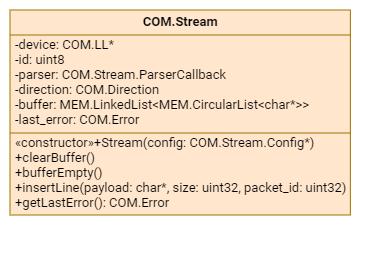
\includegraphics[width=0.4\textwidth]{./img/navig-class-stream.png}
	\caption {COM::Stream interface and members}
	\label{fig:navig-class-stream}
	\end{figure}


The \textbf{COM::RedundancyEngine} module allows several related streams "connect" and "disconnect" to and from it and compares the information between them resolving conflicts and missing information. The latter of which can be accessed through a call \texttt{resolve()}.

\begin{figure}[H]
	\centering
	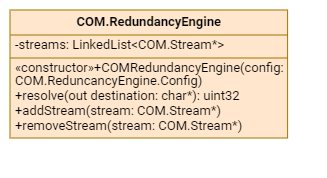
\includegraphics[width=0.35\textwidth]{./img/navig-class-redundancy-engine.png}
	\caption {COM::RedundancyEngine interface and members}
	\label{fig:navig-class-redundancy-engine}
	\end{figure}


The \textbf{COM::Manager} module is a higher level when compared to the others, it connects the tools of the other modules to create an interface that allows quick and intuitive communication setup and automatization of processes such as redundancy management.
\begin{figure}[H]
	\centering
	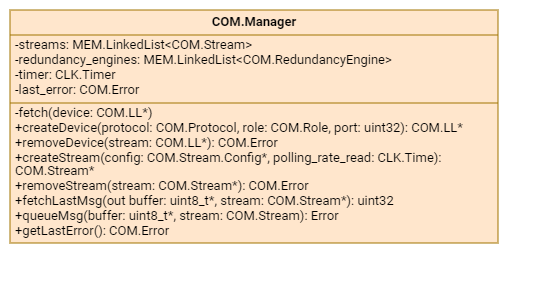
\includegraphics[width=0.5\textwidth]{./img/navig-class-manager.png}
	\caption {COM::Manager interface and members}
	\label{fig:navig-class-manager}
	\end{figure}



%//////////////////////////////// # OS Package /////////////////////////////////
\subsubsection{OS: Scheduler Package}
\label{sec:osPack}
The modules in the \textbf{OS} package mainly serve the purposes of thread creation and management management, inter-thread synchronization and thread-safe access to memory. Therefore, they all revolve around threaded execution although each fills in the need for a special bit of functionality.

The \textbf{OS::Thread} module provides a platform-agnostic interface for creating an object that will use native types and interfaces that allow each object to behave like a separate execution thread. The provided controls for it include execution and sleep mechanisms as well as options for waiting for the end of their execution and detaching threads from the parent thread. Scheduling can be managed with the options concerning thread priority and for the possibility of creating static threads it also provides the chance of delimiting the stack size. 

\begin{figure}[H]
	\centering
	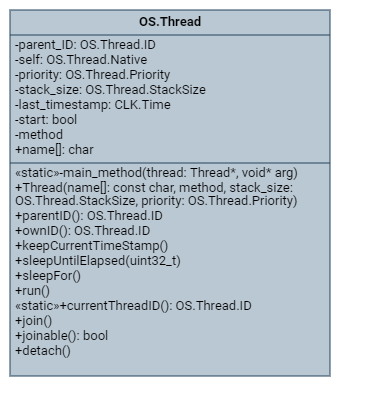
\includegraphics[width=0.4\textwidth]{./img/navig-class-thread.png}
	\caption {OS::Thread interface and members}
	\label{fig:navig-class-thread}
	\end{figure}


The \textbf{OS::Mutex} module provides a way for controlling access to shared resources that are not defined as thread-safe, which is any object that the user might create that is not of any of the modules in the High-level Hardware Abstraction Layer. It can be locked (\texttt{lock()}) in one thread in order to block access to a specific excerpt of code and it can only be locked again by the same thread or any other after it is unlocked (\texttt{unlock()}) by whatever thread locked it. It is thus non-recursive, which means that any thread, including the thread that locked in blocked in the call to \texttt{lock()} it until it is unlocked.

\begin{figure}[H]
	\centering
	\includegraphics[width=0.15\textwidth]{./img/navig-class-mutex.png}
	\caption {OS::Mutex interface and members}
	\label{fig:navig-class-mutex}
	\end{figure}


The \textbf{OS::SharedMemory} module, one the other hand, provides a platform for sharing resources between specific threads. It may be considered an expansion upon \textbf{OS::Mutex} that is specifically tailored to be used in memory protection and can reduce the roster of threads that get access to a certain memory area. 


\begin{figure}[H]
	\centering
	\includegraphics[width=0.25\textwidth]{./img/navig-class-sharedmemory.png}
	\caption {OS::SharedMemory interface and members}
	\label{fig:navig-class-sharedmemory}
	\end{figure}


\textbf{OS::Notification} is a small module that provides the inter-thread synchronization method known as a signal or a notification. A call to \texttt{wait()} from one thread will make it halt until a call for \texttt{notifyOne()} that targets it is given from another thread. A call to \texttt{notifyAll()} will notify all threads. 


\begin{figure}[H]
	\centering
	\includegraphics[width=0.28\textwidth]{./img/navig-class-notification.png}
	\caption {OS::Notification interface and members}
	\label{fig:navig-class-notification}
	\end{figure}


\subsubsection{MEM: Memory Structures Package}

The \textbf{MEM} package includes modules that offer typical containers such as linked lists and circular lists that are tightly contained and thread-safe. These are very practical ways of implementing those types of structures in heavily threaded applications as they provide easy-to-use interfaces, low-complexity operations and guarantee safe access to the resources when shared by multiple threads. 
\newline
Both \textbf{MEM::CircularList} and \textbf{MEM::LinkedList} provide interfaces for inserting and removing objects, retrieving basic information about their state, such as their size and a means to empty the list in an efficient fashion. They both also implement the universal error reporting interface with a specific type for such errors, \textbf{MEM::Error}. When making specific operations the user can also choose how the container should react when another thread of execution is accessing the structure: in \textbf{MEM::BlockingMode BLOCKING} mode, the list will wait until the resources are freed and in \textbf{NON\_BLOCKING} mode, in the same situation it will return with an error code.
\newline
The \textbf{MEM::CircularList} provides a medium for creating a fixed-size First-In-First-Out (FIFO) container to which the user can push a single or multiple objects and retrieve them in a similar fashion. 

\begin{figure}[H]
	\centering
	\includegraphics[width=0.4\textwidth]{./img/navig-class-circularlist.png}
	\caption {MEM::CircularList interface and members}
	\label{fig:navig-class-circularlist}
	\end{figure}

The \textbf{MEM::LinkedList} prioritizes quick insertion at the front or the back of any list and removal of specific objects from anywhere in the list with the same complexity. It it optimized exclusively for operations with single objects.

\begin{figure}[H]
	\centering
	\includegraphics[width=0.4\textwidth]{./img/navig-class-linkedlist.png}
	\caption {MEM::LinkedList interface and members}
	\label{fig:navig-class-linkedlist}
	\end{figure}


The modules within this package are mainly used by the \textbf{IO} and \textbf{COM} class modules for buffering information and storing objects in lists where insertions and removals need to be fast but they can also be used by higher-level classes due to their \textbf{versatile interfaces} and \textbf{general-purpose} nature.


%//////////////////////////////// # CLK Package ////////////////////////////////

\subsubsection{CLK: Timing Package}

The \textbf{CLK} package is comprised by only the \textbf{Timer} module and convenient type definitions. It provides a means for setting up repeated timed delays and executing a specific routine automatically when each delay ends. It also provides an interface for waiting for the end of the timed delay and/or the execution of the specified routine and autonomously notifies all waiting objects of these events.
It is mainly used by the \textbf{IO::GPIO} class for timing conversions but it can as easily be used by higher-level classes due to its \textbf{versatile interface} and \textbf{general-purpose} nature.

\begin{figure}[H]
	\centering
	\includegraphics[width=0.43\textwidth]{./img/navig-class-timer.png}
	\caption {CLK::Timer interface and members}
	\label{fig:navig-class-timer}
	\end{figure}



%//////////////////////////////// # APP Package ////////////////////////////////

\subsubsection{APP: Main Application Package}

The main application package is comprised by  


%
\section{Physical Environment Virtual Subsystem}%
\label{sec:phys-envir-virt-design}
%The Navigation subsystem hosts the core of the system functionality-wise, which is the control routine. This means that it should strive to not only make accurate readings and calculations but also be as efficient as possible in managing those processes in order to introduce very little delay and meet timing requirements. 

To meet these requirements as best as possible it should be capable of :

\begin{itemize}
    \item Gathering information from the physical domain at equally distant instants $kT_s$ and output an electrical representation of the command variable at equally distant instants $kT_o$;
    \item Acquiring commands from the Smartphone and Remote Vision Subsystems, identifying matches that will allow it to validate those commands and feeding them into the control rule in a useful format;
    \item Providing real-time feedback to the user about its status.
\end{itemize}


The first task should be idealizing the control system itself, understanding what inputs are needed to control the machine and then how it could be used to manipulate the wheels of the car. After that, the rest of system should be designed to fit the needs of the control rules and algorithms and use them to react as fast and consistently as possible within its own constraints and those of the other subsystems.
%
%\section{Remote Vision Virtual Subsystem}%
%\label{sec:remote-visi-subsyst-design}
\section{Remote Vision Virtual Subsystem}%
\label{sec:remote-visi-subsyst-design}
The design specification devised in
Section~\ref{sec:remote-visi-subsyst-design} can now be implemented to the
target platform to fulfill the remote vision and telemetry functionalities
required. In this section the relevant implementation details are
addressed on the hardware and software domains.
%
\subsection{Hardware}%
\label{sec:hardware-rvvs-implem}
In the design stage, and in the first iterations of the
implementation, it is perfectly reasonable to adopt general domain environments,
such as virtual machines. Nonetheless, one must keep in mind that, ultimately,
the devised software will be running on hardware nodes. Thus, an important implementation step is the selection of the target
platform, taking into considerion several design criteria, such as, throughput,
memory footprint, storage, response time, connectivity, etc.

An example of a viable platform is the Raspberry Pi Zero W (Fig.~\ref{fig:pi-zero-w}), which is a low cost
board design (it retails for about 5 EUR) around the Broadcom system on-chip (SoC) BCM2835, which includes a
1 GHz single-core ARMv6 CPU, with a 64-bit architecture, allowing it to run
the full range of GNU/Linux distribution. Among other resources, it includes 512
MB RAM, VideoCore IV GPU, 40 GPIO pins, mini HDMI and micro-USB ports,
\gls{csi} connector, Micro SD Card Slot and on-board Bluetooth Low Energy (BLE)
4.1 and Wi-Fi based.

The Raspberry Pi Zero W provides the required communications
(Bluetooth and Wi-Fi) and camera interfaces, on a fully-fledged environment
capable of running 64-bit OS and at low cost, thus, making it
suitable for the implementation. Additionally, it packs in a small form-factor,
even with the inclusion of the camera, as illustrated in
Fig.~\ref{fig:pi-zero-w-cam}. The camera module has several models ranging from
5 to 12 megapixel resolution with high quality video capture (up to 1080p30) in
the 20--35 EUR pricepoint.
%
% Pi Zero W
\begin{figure}[!hbt]
\centering
    \includegraphics[width=0.6\textwidth]{./img/pi-zero-w.png}
  \caption{Raspberry Pi Zero Wireless overview}%
\label{fig:pi-zero-w}
\end{figure}
% Pi Zero W Camera
\begin{figure}[!hbt]
\centering
    \includegraphics[width=0.6\textwidth]{./img/pi-zero-w-cam.jpg}
  \caption{Raspberry Pi Zero Wireless overview}%
\label{fig:pi-zero-w-cam}
\end{figure}
%
%
\subsection{Software}%
\label{sec:software-rvvs-implem}
The software part is mainly comprised of two main components: the software
environment support and the actual software running on top of that. The software
environment provides the low-level layer(s) that interfaces the hardware,
typically under some form of an \gls{os} and the associated development
toolchain required to target the platform.

In the present case, the selected platform --- Raspberry Pi --- supports
64-bit GNU/Linux based operating systems, which can be used to bootstrap the
implementation. Nonetheless, it is desirable to maintain the code footprint and
dependencies as low as possible, as required in the majority of the embedded
systems, thus, a custom tailored Linux OS can be used. Contemplating the build
tools required for the deployment of a tailored Linux OS, there are several
solutions, such as, Buildroot, Yocto and OpenWRT. The selected build tool was
Yocto, an open-source project project that provides templates, tools, and
methods to help you create custom Linux-based systems for embedded products
regardless of the hardware architecture~\cite{yocto2020}. Additionally, it is
required the cross-compilation toolchain that enables deployment to target from
host. Yet, in this initial implementation phase, the \gls{rvvs} susbsystem is
virtualized in a Linux \gls{vm}, thus, sparing this step for now. However, after
implementing and testing the application in the Linux \gls{vm}, this approach
should be relatively straightforward, enabling fast deployment to the real
hardware.

Hence, in the following sections, it is discussed the implementation of the
\gls{rvvs} stack designed in Section~\ref{sec:subsyst-decomposition-rvvs}.
%
\subsubsection{Image Acquisition}%
\label{sec:img-acq-rvvs-implem}
The usage of the Linux \gls{vm} has another inherent advantage, associated to
the UNIX philosophy in which it is based, that everything is a file (except for
the network part). As a matter of fact, every device attached to the Linux OS
can be easily and transparently accessed, e.g., via the \texttt{/dev}
directory. Additionally, as every device is a file, the file \gls{api} can be
used to manage the device, using the typical system calls \texttt{open/close}
and \texttt{read/write}.  

The typical call stack for image acquisition and streaming is comprised of:
low-level drivers that interface the hardware via the kernel (dependent on the
type of interface), dealing with frame capture (e.g., \gls{v4l}); and the
commonly named \emph{frame grabber}, which takes the raw frames and encodes it
into streams, for posterior multiplexing into their final container (e.g.,
\texttt{ffmpeg}).

The \gls{v4l2} is the second version of the \gls{api} and framework, which is an
integral part of the Linux kernel code, as opposed to many driver
implementations~\cite{v4l2-headers}. The \gls{v4l2} \gls{api} is mostly
implemented as set of \texttt{ioctl} (control device) system
calls~\cite{kerrisk2010linux} that enable easy manipulation of video devices.
\emph{The workflow for a typical \gls{v4l2} application is as follows}:
\begin{enumerate}
\item Open a descriptor to the device;
\item Retrieve and analyse the device's capabilities. V4L2 allows you to query a
  device for its capabilities, that is, the set of operations (roughly, IOCTL
  calls) it supports;
\item Set the capture format: frame size, format (MJPEG, RGB, YUV, \ldots),
  etc.; check the device handles the format.
\item Prepare the device for buffer handling. When capturing a frame, it has
  to submitted a buffer to the device (\texttt{queue}), and retrieved it once
  it's been illed with data (\texttt{dequeue}). However, before this, the device
  must be informed about the buffers (buffer request).
\item For each buffer, certain aspects must be negotiated with
  the device (buffer size, frame start offset in memory), and then created a new
  memory mapping for it.
\item Put the device into streaming mode.
\item Once the buffers are ready, it is only required the queueing/dequeuing
  of the buffers repeatedly, and every call will grab a new frame. The delay
  defined between each frames by putting the program to sleep is what
  determines the framerate.
\item Turn off streaming mode.
\item Close your descriptor to the device.
\end{enumerate}

The \gls{v4l2} \gls{api} is implemented in the \texttt{C} programming
language. Thus, a basic wrapper class was implemented in \texttt{C++} to
abstract from the low-level details and increase modularity, following the
aforementioned workflow.

Listing~\ref{lst:webcam-h} provides the webcam interface (public and private)
using the V4L2 API. The construtor takes the type of capture to perform, e.g.,
video capture, and the associated memory type. The open/close member functions
enable the opening and closing of the file descriptior associated with the
device. \texttt{setFormat} sets the image format and dimensions,
\texttt{startStream} starts the stream and writes the output to a file, and
\texttt{setRequestBuffer} defines the number of buffers to use. In the private
interface lies the \texttt{allocateBuffer} and \texttt{open} member functions which allocates a
buffer for the device on behalf of the \texttt{setRequestBuffer}. As private
variables there are the file descriptor associated with the device
\texttt{m\_FileDescriptor}, the pointer to a buffer frame \texttt{m\_bufferPtr},
and the V4L2 variables representing the buffer's type, memory type and
capabilities, respectively. Additionally, a mutually exclusive object variable
\texttt{m\_mutex} is used to manage concurrent access to the device via file descriptor.\\
% Webcam header file
\lstinputlisting[language=C++, caption={Webcam wrapper interface using the V4L2 API},label=lst:webcam-h,
style=customc]{./listing/webcam-v4l2.h}%

Next, a small driver program (Listing~\ref{lst:webcam-main}) was devised to test
the webcam interface. The device location is set to \texttt{/dev/video0} where
the attached camera is placed under Linux filesystem. A webcam object is created
for video capture and then is tried out the aforementioned workflow by opening
the device, setting the dimensions to 320x240 pixels and the format to Motion
JPEG (MJPEG), requesting one buffer, starting the stream to an output file and
finally closing the device.\\ 
% Webcam main
\lstinputlisting[language=C++, caption={Webcam driver program},label=lst:webcam-main,
style=customc]{./listing/webcam-main.cpp}%

Later on, the client code that uses the Webcam interface was added to
respective thread, responsible for starting a webcam stream on user-demand.
%
\subsubsection{Wi-Fi}%
\label{sec:wi-fi-rvvs-implem}
For the implementation of the Wi-Fi communication, \gls{tcpip} sockets were used
in conjunction with the client/server architecture. Although only the server is
running on the \gls{rvvs} subsystem, the instantiation of both client and server
enables the testing of the complete communications workflow, without the need to
add the uncertainty associated with the communication medium.


%  UTILITY FUNCTIONS:
%  One must specially careful with the byte ordering (aka endianess), so one does not get
%  "translations" mistakes. In that sense, one must remember two things:
%  	1. The network byte ordering is always big endian.
%  	2. Before sending data packets to the network, one must always convert it to 
%          network byte ordering.
%  For this purpose, we use the following utility functions:
%  + Byte Ordering:
%   - Host Byte Order to Network Byte Order:
%   	- short: htons();
%   	- long:  htonl().
%   - Network Byte Order to Host Byte Order:
%   	- short: ntohs();
%   	- long:  ntohl();
%
%  + IP Adress format:
%   - ASCII dotted to Binary: inet_aton()
%   - Binary to ASCII dotted: inet_ntoa()
%  
%  + Padding
%   - bzero: write zeroes to a byte string
%   	bzero(void *s, size_t n);

%
%%% Local Variables:
%%% mode: latex
%%% TeX-master: "../../../dissertation"
%%% End:

%
\section{Smartphone}%
\label{sec:smartphone-design}
%\section{Smartphone}%
%\label{sec:smartphone-design}
The smartphone design was divided into three stages, the functional model, the object model and the dynamic model.

\subsection{Functional Model}
The functional model includes a description of the system in terms of accessible functionalities from the actors' point of view, represented in figure \ref{fig:usecase_android}.
%
In this stage, the actors identified were the user, the \gls{nvs} and the \gls{rvvs}. The user must have access to three key features:
% 
\begin{itemize}%
\item \textbf {Vehicle control}: the ability to control the car by tilting the smartphone and thereby changing the provided angle and speed reference. This feature implies a transmission of these values to the \gls{nvs} and a UI value update.
\item \textbf {Notification view}: pop-ups that allow a grasp of the current state of the system with informative or alert messages.
\item \textbf {Video feed view}: Be able to visualize the \gls{rvvs}` video transmission on screen.
\end{itemize}
%
On one hand, the \gls{nvs} should be able to receive the accelerometer data provided while also sending notifications to the app, both via Bluetooth.
%
On the other hand, the \gls{rvvs} should be capable of transmitting the camera´s video while also sending the same type of notifications to the user within the application. This communication is established via Wifi/GPRS.
%
\begin{figure}[!ht]
\centering
\includegraphics[width=0.8\textwidth]{img/UseCaseAndroid.png}
\caption{\label{fig:usecase_android}Android app use case diagram.}
\end{figure}
%
\subsection{Object/Static Model}
In this step, the objective was to define the app system´s structure with \gls{uml} class diagrams, concerning its objects, attributes, operations and associations established.  The forementioned diagram is represented in figure \ref{fig:uml-android}.
%
\begin{figure}[!ht]
\centering
\includegraphics[width=\textwidth]{img/smartphone-static-diagram.png}
\caption{\label{fig:uml-android}Smartphone class diagram}
\end{figure}
%
\subsection{Dynamic Model}
For the dynamic model, were devised multiple state-machine diagrams to describe the internal behaviour of the application. 
%
Figure \ref{fig:overall_system_diagram} illustrates the overall application behaviour. One can observe that all the intended features are meant to run in parallel, that will surely affect the system implementation in terms of concurrency (section \ref{sec:concurrency}) and thread management.
%
Initially, the system loads the \gls{ui} and waits for all connections to be established before moving to the next state.
%
While the feature for vehicle control is running (figure \ref{fig:vehicle_control_diagram}) it retrieves the accelerometer data, sends the data to the \gls{nvs} and displays it on the screen.
%
Additionally, the feature that allows the user to see the video feed transmitted by the \gls{rvvs} in figure \ref{fig:video_feed_diagram} also displays it on the app screen. When this Wifi/GPRS connection is suspended by any means, it should exist an immediate reconnection to the \gls{rvvs}.
%
The notifications presented to the user should indicate the current state of the system, which means displaying informative messages, like successful connections but also alert messages like the ones displayed in figure \ref{fig:notification_diagram}.
%
\begin{figure}[!ht]
\centering
\includegraphics[width=0.7\textwidth]{img/overall_system_sm.png}
\caption{\label{fig:overall_system_diagram}Overall system behaviour diagram.}
\end{figure}
%
\begin{figure}[!ht]
\centering
\includegraphics[width=0.7\textwidth]{img/vehicle_control_sm.png}
\caption{\label{fig:vehicle_control_diagram}Vehicle control feature diagram.}
\end{figure}
%
\begin{figure}[!ht]
\centering
\includegraphics[width=0.7\textwidth]{img/video_feed_sm.png}
\caption{\label{fig:video_feed_diagram}Video feed feature diagram.}
\end{figure}
%
\begin{figure}[!ht]
\centering
\includegraphics[width=0.7\textwidth]{img/notification_sm.png}
\caption{\label{fig:notification_diagram}Notification feature diagram.}
\end{figure}
%
%
%\section{Hardware/Software mapping}%
%\label{sec:hw-sw-mapping}
\section{Hardware/Software mapping}%
\label{sec:hw-sw-mapping}
In the hardware/software mapping activity, the functionality associated to a
software component is mapped to the hardware responsible for executing it. It is
represented by a UML deployment diagram used to depict the relationship between
run-time components and nodes.
Components are self-contained entities that
provide services to other components or actors, e.g., the \texttt{RVVS\_App} in
Fig.~\ref{fig:deployment-diag}.
A node is a physical device or an execution environment in which components are
executed, such as a desktop computer, or \texttt{myLinux} in Fig.~\ref{fig:deployment-diag}, represented by boxes containing
component icons. Furthermore, a node can contain another node, for example a
device can contain an execution environment such as virtual machine.

The UML deployment diagram for the \gls{rfcar} system is depicted in
Fig.~\ref{fig:deployment-diag}, where the two nodes --- Smartphone and LinuxVM
--- are represented in turquoise and orange, respectively. The ball-and-socket
joint identifies the provided and required interfaces, respectively. Thus, the
\texttt{RVVS\_app} provides wireless communication interfaces that the
\texttt{Android\_app} can use, namely Wi-Fi and GPRS~.
Furthermore, it highlights the client-server software pattern, with the
\texttt{RVVS\_app} and \texttt{NVS\_app} serving the requests (servers) that the
\texttt{Android\_app} requests (client).
The \texttt{Android\_app} communicates with the \texttt{NVS\_app} via Bluetooth,
or, if the communications fail, through any of the available communications
channels for the \texttt{RVVS\_app} that forwards that request for
\texttt{NVS\_app}.

Lastly, it should be noted that in a real-world scenario the \texttt{NVS\_app}
and \texttt{RVVS\_app} are mapped to a different hardware, which is also distinct
between them, e.g., the former in an \texttt{STM32} and the latter in a
\texttt{Raspberry Pi}. However, in the virtualized environment, and ideally,
they represent two distinct processes that must communicate via an \gls{ipc}
mechanism, e.g., sockets. Nonetheless, to ease and speed up the development it
is perfectly acceptable to implement both processes into the same application in
the early development phase.
% Deployment diagram
\begin{figure}[!hbt]
\centering
    \includegraphics[width=0.7\textwidth]{./img/deployment-diag.pdf}
  \caption{\acrshort{rfcar} Deployment diagram}%
\label{fig:deployment-diag}
\end{figure}
%
%%% Local Variables:
%%% mode: latex
%%% TeX-master: "../../../dissertation"
%%% End:

%
%
%%% Local Variables:
%%% mode: latex
%%% TeX-master: "../../../dissertation"
%%% End:

  \setcounter{table}{0}
  \setcounter{figure}{0}
  %%\begin{document}
% CHAPTER - Contribution -------------------------
\chapter{Development}
\label{ch:development}
%
In this chapter, the knowledge acquired through the relevant models contained

The implementation of this thread is presented
in listing~\ref{lst:threadSerialRx}.
%
% LISTING: ThreadSerialRx
\lstinputlisting[language=C++, caption={Thread Serial Rx handler},label=lst:threadSerialRx,
style=customc]{./listing/threadSerialRx.cpp}%

%


%
%%% Local Variables:
%%% mode: latex
%%% TeX-master: "../../../dissertation"
%%% End:

  % CHAPTER - Implementation ---------------
\chapter{Implementation}%
\label{ch:implementation}
In the implementation phase, the solution developed in the various domains is
implemented into the target platforms, accordingly to the system design
specification. In this chapter is presented the implementation for the various domains and subsystems identified.
%
\section{Navigation Virtual Subsystem}%
\label{sec:navig-virt-subsyst-implem}
%The Navigation subsystem hosts the core of the system functionality-wise, which is the control routine. This means that it should strive to not only make accurate readings and calculations but also be as efficient as possible in managing those processes in order to introduce very little delay and meet timing requirements. 

To meet these requirements as best as possible it should be capable of :

\begin{itemize}
    \item Gathering information from the physical domain at equally distant instants $kT_s$ and output an electrical representation of the command variable at equally distant instants $kT_o$;
    \item Acquiring commands from the Smartphone and Remote Vision Subsystems, identifying matches that will allow it to validate those commands and feeding them into the control rule in a useful format;
    \item Providing real-time feedback to the user about its status.
\end{itemize}


The first task should be idealizing the control system itself, understanding what inputs are needed to control the machine and then how it could be used to manipulate the wheels of the car. After that, the rest of system should be designed to fit the needs of the control rules and algorithms and use them to react as fast and consistently as possible within its own constraints and those of the other subsystems.
%
\subsection{Control}%
\label{sec:control-design}
%The Navigation subsystem hosts the core of the system functionality-wise, which is the control routine. This means that it should strive to not only make accurate readings and calculations but also be as efficient as possible in managing those processes in order to introduce very little delay and meet timing requirements. 

To meet these requirements as best as possible it should be capable of :

\begin{itemize}
    \item Gathering information from the physical domain at equally distant instants $kT_s$ and output an electrical representation of the command variable at equally distant instants $kT_o$;
    \item Acquiring commands from the Smartphone and Remote Vision Subsystems, identifying matches that will allow it to validate those commands and feeding them into the control rule in a useful format;
    \item Providing real-time feedback to the user about its status.
\end{itemize}


The first task should be idealizing the control system itself, understanding what inputs are needed to control the machine and then how it could be used to manipulate the wheels of the car. After that, the rest of system should be designed to fit the needs of the control rules and algorithms and use them to react as fast and consistently as possible within its own constraints and those of the other subsystems.
%
\section{Physical Environment Virtual Subsystem}%
\label{sec:phys-envir-virt-design}
%The Navigation subsystem hosts the core of the system functionality-wise, which is the control routine. This means that it should strive to not only make accurate readings and calculations but also be as efficient as possible in managing those processes in order to introduce very little delay and meet timing requirements. 

To meet these requirements as best as possible it should be capable of :

\begin{itemize}
    \item Gathering information from the physical domain at equally distant instants $kT_s$ and output an electrical representation of the command variable at equally distant instants $kT_o$;
    \item Acquiring commands from the Smartphone and Remote Vision Subsystems, identifying matches that will allow it to validate those commands and feeding them into the control rule in a useful format;
    \item Providing real-time feedback to the user about its status.
\end{itemize}


The first task should be idealizing the control system itself, understanding what inputs are needed to control the machine and then how it could be used to manipulate the wheels of the car. After that, the rest of system should be designed to fit the needs of the control rules and algorithms and use them to react as fast and consistently as possible within its own constraints and those of the other subsystems.
%
\section{Remote Vision Virtual Subsystem}%
\label{sec:remote-visi-subsyst-design}
%The Navigation subsystem hosts the core of the system functionality-wise, which is the control routine. This means that it should strive to not only make accurate readings and calculations but also be as efficient as possible in managing those processes in order to introduce very little delay and meet timing requirements. 

To meet these requirements as best as possible it should be capable of :

\begin{itemize}
    \item Gathering information from the physical domain at equally distant instants $kT_s$ and output an electrical representation of the command variable at equally distant instants $kT_o$;
    \item Acquiring commands from the Smartphone and Remote Vision Subsystems, identifying matches that will allow it to validate those commands and feeding them into the control rule in a useful format;
    \item Providing real-time feedback to the user about its status.
\end{itemize}


The first task should be idealizing the control system itself, understanding what inputs are needed to control the machine and then how it could be used to manipulate the wheels of the car. After that, the rest of system should be designed to fit the needs of the control rules and algorithms and use them to react as fast and consistently as possible within its own constraints and those of the other subsystems.
%
\section{Smartphone}%
\label{sec:smartphone-implem}
%\section{Smartphone}
%\label{sec:smartphone-implem}
The mobile \gls{os} chosen for this project was \textbf{Android}. Usually, android apps can be implemented using Kotlin, Java and C++. For the \gls{rfcar} project, the language chosen was \textbf{Java} due to the knowledge gained in prior course years where the need to implement android-targeted applications rose. Additionally, the code was conceived using the \textbf{Android Studio} \gls{ide}. One must notice that despite the user-friendliness of the development environment through context-sensitive guidelines and code suggestions, this language and \gls{ide} are not the best in terms of full system control due to the multiple abstraction layers preemptively defined. Therefore, one might wonder why the C++ route with a cross-platform framework like QT wasn't selected. Multiple options were taken into account at this stage and its a fact that the one that ended up being selected might not deliver as much implementation freedom as the second option forementioned. However, it allowed deadline fulfilment and code reuse notwithstanding the additional effort put into delving deeper within some contexts.
%
\subsection{Sensor Interaction}%
\label{sec:accelerometer-access}
%
The smartphone has a built-in MEMS accelerometer, this means that at micro-level it can measure acceleration values through capacitance changes in multiple capacitors as a result of its internal assembly (calibration mass and spring contacts) displacement. With at least a MEMS system in each plane (x,y,z), one can measure the acceleration per axis. 
\subsubsection{Sensor Data Retrieval}
\label{sec:accelerometer-data}
%
The code in listing ~\ref{lst:get_accelerometer_vals} (based on \cite{androiddevsensors}) represents the retrieval of the linear acceleration for each plane.
In the first place, the definition of the sensor type is crucial to access its values (line 9). \textbf{SensorManager} grants access to the sensors of the android device (line 7). Following, one must create a listener that checks the sensors values at a determined sampling frequency using the SensorManager's method \textbf{registerListener} (line 10). Upon doing so, one overwrites the \textbf{onSensorChanged} method (line 15) so the pretended variables that hold the values of the sensor can only be updated on smartphone movement.
An acceleration sensor measures the acceleration applied to the device but regarding the force of gravity. For this reason, the values retrieved do not represent the linear accelerations for each plane. To resolve this problem, a low pass filter can be used to isolate the force of gravity in each axis (line 28) and then remove its contibution from the acceleration values (line 33).\\
%
\lstinputlisting[language=Java,caption={Accelerometer data retrieval code},label=lst:get_accelerometer_vals,style=custom-java]{listing/accelerometerAccess.java}
%
As the control module uses both wheels tilt angle and tension applied to the motor as input, the interface with the smartphone's accelerometer wasn't enough. To generate the angles necessary and vary the tension accordingly one needs to access the phone's rotation sensors. This code is implemented in listing \ref{lst:get_rot_vals}. As the interface with the accelerometer, this latter interface needs a \textbf{SensorManager} and the creation of a listener with the \textbf{registerListener} method. Some calibrations were crucial to ensure the calculated values of the angles matched the initial smartphone position chosen. Note that percentages were used as a way to implement a control independent of the motor and wheels used. This means that using a percentage of the voltage applied and wheel tilt, one could simply use a 12V or 6V motor, for example. Therefore, the control values would be immutable. This will be tested in secction \ref{sec:accelerometer-using-data-test}.\\

%
\lstinputlisting[language=Java,caption={Rotation sensor data retrieval code},label=lst:get_rot_vals,style=custom-java]{listing/rotAccess.java}
%
\subsubsection{Applying Sensor Data}
\label{sec:using-accelerometer-data}
%
The project requires that the acceleration values obtained from the sensors are applied to make the vehicle move in the intended direction with the expected speed. 
%
To implement the code referent to this sub-subsection, one must pay close attention to the axis orientation in a common device, represented in figure \ref{fig:axis-smartphone}.
%
\begin{figure}[!h]
\centering
\includegraphics[width=0.85\textwidth]{img/smartphone_axis.png}
\caption{\label{fig:axis-smartphone}Axis orientation in a smartphone}
\end{figure}
%
In order to test this concept, the code presented in \ref{sec:accelerometer-data} that refers to the accelerometer was added to another project that allowed ball movement based on the accelerometer values. It must be noticed that the z acceleration value it's not relevant to the ball movement (from line 59 to 67) since only \textbf{roll} and \textbf{pitch} affect a 2D (bidimensional) object and the smartphone height relative to the ground doesn't, as one should expect by analysing figure \ref{fig:axis-smartphone}.
%
This code in listing \ref{lst:ball_mov} representing subsection \ref{sec:accelerometer-access} will be tested in \ref{sec:accelerometer-using-data-test}.\\
%
\lstinputlisting[language=Java,caption={Code for ball movement based on accelerometer data},label=lst:ball_mov,style=custom-java]{listing/ballMovement.java}
%
%
\subsection{Bluetooth}%
\label{sec:bluetooth-implem}
%
Bluetooth is one of the communication technologies specified in the project analysis (section \ref{ch:analysis}), hence it is important to assure the data flow between the smartphone and the \gls{nvs} on another redundancy communication failure like Wi-Fi. 
%
\subsubsection{Bluetooth Connection Setup}
\label{sec:bluetooth-connection-setup}
Starting from the design and reusing previous Java code made on other course units (based on \cite{btchatsrc}), the Bluetooth setup was implemented on Android Studio and then deployed in a smartphone, the code is depicted in listing \ref{lst:bt-setup}.
%
Note that the forementioned code has \textbf{threads} to simulate parallel computing since the app should be able to send data to the paired device and receive data from it.
%
In lines 10, 11 and 12, are represented the three thread classes used for the Bluetooth connection setup. These classes inherit from the \textbf{Thread class} (\underline{extends Thread} - line 114), considering it must exist \textbf{concurrency} and \textbf{resource sharing} for the application to send and receive data simultaneously. 
%
The \textbf{AcceptThread} (line 10) it's related to the discovery of new connections since it plays an important role in the creation of a \textbf{BluetoothServerSocket} that allows two intended devices to find and accept each other as a part of the initial device inquiry prior to the connection stage. Line 11 represents the \textbf{ConnectThread} responsible for managing the connection between two devices. This thread starts as soon as the two devices accept each other and then proceeds to create a \textbf{RfcommSocket} and connect the devices (pair) when the user clicks on an unpaired device from the list presented. Finally, the \textbf{IOThread} assures the message exchange between devices by accessing the input and output streams of the \textbf{Bluetooth Socket}.
%
As stated earlier, it was necessary to make some includes in the Bluetooth app as well as virtualize some ports in order to interface the \gls{pc} virtual machine with the smartphone, this will be more thoroughly explained in the testing section (\ref{sec:bluetooth-phone-nvs}).
%
Finally, from the smartphone point of view, the protocol purpose was to transmit commands to control the vehicle by sending the phone accelerometers' values and receive its message warnings on screen.\\
%
\lstinputlisting[language=Java,caption={Code for bluetooth connection setup},label=lst:bt-setup,style=custom-java]{listing/btSetup.java}
%
%%% Local Variables:
%%% mode: latex
%%% TeX-master: "../../../dissertation"
%%% End:



%
%
%%% Local Variables:
%%% mode: latex
%%% TeX-master: "../../../dissertation"
%%% End:

  \setcounter{table}{0}
  \setcounter{figure}{0}
  %
  %% CHAPTER - Application -------------------------
\chapter{Tests}
\label{ch:application}
In this chapter, the \gls{lbam} methodology devised was tested and the results

% Please add the following required packages to your document preamble:
% \usepackage{multirow}
\begin{table}[!hbt]
\centering
\caption{\gls{mms} machine final specifications}
\label{tab:mach-final-specs}
\begin{tabular}{ll}
\hline
Dimensions (l x w x h){[}mm{]} & 560 x 450 x 280 \\ \hline
\multirow{2}{*}{Power supply} & Laser: 400 VAC, 10 A \\ \cline{2-2} 
 & Machine: 24 V, 15 A \\ \hline
Build dimensions {[}mm{]} & 50 x 50 x 50 \\ \hline
Nr. of materials & 2 \\ \hline
Temperature & Tested up to 250$^{\circ}$C (higher temperatures can be used) \\ \hline
\multirow{3}{*}{Laser} & Type: $CO_2$ \\ \cline{2-2} 
 & Power: 30 W \\ \cline{2-2} 
 & Spot size: 50 $\mu$m \\ \hline
  \multirow{2}{*}{Resolution {[}$\mu$m{]}} & Full-step (all axes, except bed): 5 $\pm$ 0.25 \\ \cline{2-2} 
 & 1/16-step (bed): 0.32 $\pm$ 0.016 \\ \hline
\multirow{3}{*}{Estimated cost {[}EURO{]}} & Laser: 7500 \\ \cline{2-2} 
 & Machine: 1500 \\ \cline{2-2} 
 & Total: 9000 \\ \hline
\end{tabular}
\end{table}

\section{Summary}
In this chapter tests were performed on the workflow, equipment and
%%% Local Variables:
%%% mode: latex
%%% TeX-master: "../../../dissertation"
%%% End:

  % CHAPTER - Testing ---------------
\chapter{Testing}%
\label{ch:testing}
After implementing the solution developed in the various domains into the
target platforms, the system's behaviour is tested in several levels of
granularity: at the subsystem level --- unit testing, and system level ---
integrated testing. The idea is progressively test the behaviour of each
subsystem and its integration into the system.
In this chapter are presented the unit testing and integrated testing for the \gls{rfcar}.
%
\section{Unit testing}%
\label{sec:unit-testing}
The unit tests are briefly described in this section.
    %\input{./tex/Chap/Testing/unit-testing}
    \subsection{Navigation Virtual Subsystem}%
    \label{sec:navig-virt-subsyst-test}%
The NVS susbsystem tests are presented next.
    %
%intro
The stack implementation tests were mainly focused on the interactions established between the packages at play and the surrounding systems both lower-tiered and high-tiered.
%
\subsubsection{IO: Input/Output Package}
%
The IO package testing (figure \ref{fig:io-test}) consisted in the creation of a GPIO object with which one could simulate motor PWM outputs that would generate a file, through which one would simulate the IR sensor readings or motor pulse readings. The first GPIO test relied on a configuration of an object in OUTPUT\_PWM mode. With the latter test, it was possible to write three 32 bit integers to a binary file and observe the results with notepad++.
The second test hinged on reading from the forementioned binary file, expecting to retrieve the corresponding values. Should the latter be as expected the test could be considered a success.
%
\subsubsection{COM: Communications Package}
%
The COM package testing involved effectuating some experiments between the \gls{nvs} and the smartphone (using Bluetooth) and the former and the \gls{rvvs} (using RS232). These experiments will be performed in section \ref{sec:nvs-tests}.
%
\subsubsection{OS: Scheduler Package}
%
\subsubsection{MEM: Memory Structures Package}
%
\subsubsection{CLK: Timing Package}
%
The CLK package testing (figure \ref{fig:clk-test}) included the creation of a Timer object, associating it to a callback and proceed to verify if the callback was called at the specified time preemptively defined in the Config object configuration.
%
\begin{figure}[!ht]
\centering
\includegraphics[width=0.8\textwidth]{img/IO-test.png}
\caption{\label{fig:io-test}IO package OUTPUT\_PMW mode tests}
\end{figure}
%
%
\begin{figure}[!ht]
\centering
\includegraphics[width=0.8\textwidth]{img/CLK-test.png}
\caption{\label{fig:clk-test}CLK package tests}
\end{figure}
%%
    \label{sec:nvs-tests}
    %\input{./tex/Chap/Testing/unit-testing}
    %
    \subsubsection{System response}
The implementation of the control module was made using the modified speed algorithm mentioned and explained in \ref{sec:des-pid}.\\
The tests for this module consists in the comparison between the results obtained and simulated in \ref{sec:des-sim-res}.\\
Starting with speed reference = 1 m/s and $\theta=0~\si{rad}$:
\begin{figure}[!h]
\centering
\includegraphics[width=0.7\textwidth]{./img/testv1t0.PNG}
\caption {\label{fig:test - vel0}Wheels velocity v=1m/s,$\theta = 0~\si{rad}$}
\end{figure}
In the figure \ref{fig:test - vel0} shows that the velocity of both wheels reaches the reference value in nearly 1.5 seconds, while in the simulation \ref{fig:sim1 - vel} it takes about 3 seconds. This discrepancy is due to the controller in use. The simulations  were made using the PID block provided by Simulink, while in the implementation, the controller algorithm used was as mentioned before, the modified speed algorithm. With this algorithm the behavior of the car is the same as with the traditional PID, but faster.\\
\begin{figure}[!h]
\centering
\includegraphics[width=0.7\textwidth]{./img/testx1t0.PNG}
\caption {\label{fig:test - xy0}Position v=1m/s,$\theta = 0~\si{rad}$}
\end{figure}
In the figure \ref{fig:test - xy0} it can be observed that the position of the car is the same as in the simulation \ref{fig:sim1 - pos}.\\
With speed reference = 1m/s and $\theta = 0.1~\si{rad}$:\\
\begin{figure}[!h]
\centering
\includegraphics[width=0.7\textwidth]{./img/testv1t01.PNG}
\caption {\label{fig:test - vel01}Wheels velocity v=1m/s,$\theta = 0.1~\si{rad}$}
\end{figure}
In the figure \ref{fig:test - vel01} comparing to \ref{fig:sim2 - vel} it's possible to see that once again the time it takes to reach steady state is smaller for the reason mention before. In the implemented algorithm it's also possible to see that the steady value of the velocity of both wheels has a ripple around the reference value. \\
\begin{figure}[!h]
\centering
\includegraphics[width=0.7\textwidth]{./img/testx1t01.PNG}
\caption {\label{fig:test - xy01}Position v=1m/s,$\theta = 0.1~\si{rad}$}
\end{figure}
In the figure \ref{fig:test - xy01} it is present the position of the car. In comparison to the simulated \ref{fig:sim2 - pos} it is possible to see that the results are the same, thus validating the implementation.\\
\subsubsection{Obstacle Avoidance Through Odometric Sensors}
The car composed by 9 odometric sensors radially distributed, 40 degrees apart.\\
In order to test if the car can avoid obstacles, the values for the sensors were generated, and the behavior of the car was as follows:\\
\begin{figure}[!h]
\centering
\includegraphics[width=0.7\textwidth]{./img/testodovel.PNG}
\caption {\label{fig:test - odovel}Wheels velocity}
\end{figure}

\begin{figure}[!h]
\centering
\includegraphics[width=0.7\textwidth]{./img/testodoxy.PNG}
\caption {\label{fig:test - odoxy}Car position}
\end{figure}

In the figure \ref{fig:test - odovel} it is possible to see that at t=2.5 seconds the velocity of both wheels starts decreasing until they reach a value near 0 m/s. Even though the velocity of both wheels is not exactly 0 m/s, the values are too small to break the inertia of the wheels, so the car effectively stops.
In the figure \ref{fig:test - odoxy} it is possible to see that the position of the car remains the same after the decrease of the velocity of the wheels, proving that the car is not moving.
    %
    %\subsection{Physical Environment Virtual Subsystem}%
    %\label{sec:phys-envir-virt-design}
    %\input{./tex/Chap/Testing/unit-testing}
    %
    %\subsection{Remote Vision Virtual Subsystem}%
    %\label{sec:remote-visi-subsyst-testing}
    \subsection{Remote Vision Virtual Subsystem}%
\label{sec:remote-visi-subsyst-testing}
In this section are presented the tests performed on the \gls{rvvs} subsystem in
the relevant domains.
%
\subsubsection{Image Acquisition}%
\label{sec:img-acq-rvvs-test}
The image acquisition system, implemented in
Section~\ref{sec:img-acq-rvvs-implem}, was tested out to assess its behaviour.

Firstly, it was selected the built-in webcam from host and attached to the guest
\gls{vm}. However,
and despite extensive troubleshooting, the bypass suggested for web
cameras\cite{webcam-bypass} was not possible for a Mac OS host. Thus, a quick
alternative was to flash a Linux \gls{os} onto a \gls{sd} card and plug it to a
Raspberry Pi 3 (available) and connect an external \gls{usb} camera to it (Fig.~\ref{fig:rasp-cam-test}).
% Raspberry Pi 3 camera test
\begin{figure}[!hbt]
\centering
    \includegraphics[width=0.6\textwidth]{./img/rasp-cam-test.jpg}
  \caption{Raspberry Pi 3 + Webcam testing setup}%
\label{fig:rasp-cam-test}
\end{figure}
%

The deployment was performed using the \gls{ssh} protocol to connect to the
Raspberry Pi and execute the necessary commands on it, and using the \gls{scp}
command that uses the \gls{sftp} protocol to transfer files between host and
guest (Listing~\ref{lst:deploy-cmds}).
\lstinputlisting[language=sh, caption={Deployment commands targetting Raspberry
Pi},label=lst:deploy-cmds,
style=customc]{./listing/ssh-scp.sh}%

The web camera was then tested using the \texttt{lsusb} command and piping the
output to a \texttt{.txt} file for further
examination. Listing~\ref{ref:lst:lsb-output} contains an excerpt of this output
where it can be observed the
webcam model (\texttt{Cubeternet WebCam}) and the \gls{usb}2.0 interface.
\lstinputlisting[language=sh, caption={Webcam information obtained via
  \texttt{lsusb} (excerpt)},label=lst:lsb-output,
style=customc]{./listing/lsusb-output.sh}%

However, this information by itself is not so useful. Additionally, and much
more importantly, one wants to check the capabilities of the device and the
supported formats. For that purpose it was used the \texttt{v4l2-ctl} utility
(Listing~\ref{lst:webcam-features}). It can be observed that the only format
supported is YUYV, which is a colour space based on one luminance component (Y')
and two chrominance components, called U(blue) projection and V(red projection),
respectively. The framerate is also fixed (30 fps), but with different
resolutions. This is very limitative, as the newer webcams support MJPEG
formats, easing video capture.
\lstinputlisting[language=sh, caption={Webcam supported image formats,
  resolutions, and framerates},label=lst:webcam-features,
style=customc]{./listing/webcam-features.sh}%

Effectively, it was executed the driver program for the webcam interface
(Listing~\ref{lst:webcam-main}), but it reported the unsupported format as
expected (Listing~\ref{lst:webcam-main-error}).
% webcam-main-error
\lstinputlisting[language=C++, caption={Webcam driver program error: unsupported
image format},label=lst:webcam-main-error,
style=customc]{./listing/webcam-main-error.sh}%

Then, it was tried out the \texttt{UYVY422} format by modifying the following
lines into Listing~\ref{lst:webcam-main}
(Listing~\ref{lst:webcam-main-modifs})
% webcam-main-error
\lstinputlisting[language=C++, caption={Webcam driver program error:
  modifications to support \texttt{UYVY422} format},label=lst:webcam-main-modifs,
style=customc]{./listing/webcam-main-modifs.cpp}%

Although an image in the \texttt{UYVY422} format was obtained, \texttt{ffmpeg}
requires tedious conversions between the packed format (\texttt{UYVY422}) to
planar one (\texttt{JPG}). Thus, an online tool was used to convert this image~\cite{conv-UYVY-jpg} into \texttt{jpg} format. In Fig.~\ref{fig:rasp-cam-test-succ} can be seen that an image was
successfully acquired.
% Raspberry Pi 3 camera test
\begin{figure}[!hbt]
\centering
    \includegraphics[width=0.6\textwidth]{./img/webcam-test-success.jpg}
  \caption{Raspberry Pi 3 + Webcam test: success}%
\label{fig:rasp-cam-test-succ}
\end{figure}

However, this is a tedious process that could be avoided by using a different,
newer, web camera supporting additional formats and resolutions, which limited
severely the implementation and testing.
%
%%% Local Variables:
%%% mode: latex
%%% TeX-master: "../../../dissertation"
%%% End:

    %
    \subsection{Smartphone}%
    \label{sec:smartphone-testing}
    %
%
\subsubsection{Bluetooth}%
\label{sec:bluetooth-test}
After effectively changing the direction of a ball according to the accelerometer's state in the section \ref{sec:accelerometer-using-data-test}, one could only need to merge its code with the Bluetooth connection setup, so that, instead of sending plain text messages, one can transfer the acceleration values.
%
\subsubsection{Bluetooth: Smartphone-Smartphone}%
\label{sec:bluetooth-phone-phone}
%
The first test was based on testing the Bluetooth connection setup when the interface was comprised of two distinct smartphones. With that in mind, the connection was successful and the devices were able to exchange messages, as expected. Since this test was performed using the code done in another course unit no further in-depth explanations will be presented in this section as the code was fully functional.
%
\subsubsection{Bluetooth: Smartphone-NVS}%
\label{sec:bluetooth-phone-nvs}
%
An initial test was made with the \textbf{HC-05 Bluetooth module} inserted on the STM board. That approach only allows system engineers who have access to that module to fully test both Bluetooth client and server. 
%
However, to prove this new compound functionality, the device to be paired should also have Bluetooth drivers (setup) and specific hardware to use that protocol.
%
However, despite both devices having the forementioned drivers and hardware for the connection to succeed, that didn't happen. After some research on the topic, one can assume that the problem was caused by \textbf{android version mismatching}. Meaning that the \underline{HC-05 only recognised older android versions (prior to 4.2)}.
%
Fortunately, a new solution was found where one could run the server Bluetooth app in a virtual machine using, for example, COM6 port to communicate, and then redirect that port to another one (COM9) establishing the connection with the phone. In other words, the android app and bluetooth server app can be connected to different ports and still comunicate, due to the foresaid redirection represented in figure \ref{fig:port-red}. As an advantage, this method requires less hardware resources.
%
\begin{figure}[!ht]
\centering
\includegraphics[width=0.5\textwidth]{img/port-red.png}
\caption{\label{fig:port-red}Port redirection}
\end{figure}
%
After turning on Bluetooth on both android (ram) and PC devices (JOAO F), as depicted in figure \ref{fig:bt_app_pc}, one could then open the android app and see in main menu its initial functionalities, figure \ref{fig:bt_intro_main}. The app manually requests Bluetooth enabling if it isn't in the beginning.
%
\begin{figure}[!ht]
\centering
\includegraphics[width=0.9\textwidth]{img/bt_app_pc.png}
\caption{\label{fig:bt_app_pc}Smartphone as "ram" and PC as "JOAOF" with Bluetooth on}
\end{figure}
%
\begin{figure}[!ht]
\centering
\includegraphics[width=0.5\textwidth]{img/bt_intro_main.png}
\caption{\label{fig:bt_intro_main}BTapp: Initial and main activities, accordingly}
\end{figure}
%
\begin{figure}[!ht]
\centering
\includegraphics[width=0.7\textwidth]{img/bt_disc_list_setup.png}
\caption{\label{fig:bt_disc_list_setup}BTapp: Discoverable, Start Listening and Connection Setup activities, respectively}
\end{figure}
%
To make an initial connection from square one, the smartphone should be discoverable and then be able to start listening, so that one could configure its connection setup. To do that, the options available in the main menu were clicked in that sequence, and when making it discoverable (even if only for 300 seconds) one should accept, figure \ref{fig:bt_disc_list_setup}.
%
\begin{figure}[!ht]
\centering
\includegraphics[width=0.4\textwidth]{img/bt_con_scan_pair_suc.png}
\caption{\label{fig:bt_con_scan_pair_suc}BTapp and PC: Pressed Scan Devices button, target device pressed and paired successfull message on PC. A PIN number given by the PC must be inserted on app to conclude the pair phase}
\end{figure}
%
\begin{figure}[!hbt]
\centering
\includegraphics[width=0.4\textwidth]{img/bt_failed_pair.png}
\caption{\label{fig:bt_failed_pair}BTapp: Pair failed examples: Wrong pin number or already paired device}
\end{figure}
%
\begin{figure}[!hbt]
\centering
\includegraphics[width=0.5\textwidth]{img/bt_sequence_connect.png}
\caption{\label{fig:bt_sequence_connect}BTapp: Connect phases: List devices pressed, target deviced pressed and successfull display of connection establish toast}
\end{figure}
%
\begin{figure}[!hbt]
\centering
\includegraphics[width=0.5\textwidth]{img/bt_sendapp_recpc.png}
\caption{\label{fig:bt_sendapp_recpc}BTapp and PC BT server: Successfull message exchanged from android to pc and android echo}
\end{figure}
%
\begin{figure}[!hbt]
\centering
\includegraphics[width=0.5\textwidth]{img/bt_sendPC_recAPP.png}
\caption{\label{fig:bt_sendPC_recAPP}BTapp and PC BT server: Successfull message exchanged from pc to android}
\end{figure}
%
\begin{figure}[!hbt]
\centering
\includegraphics[width=0.3\textwidth]{img/bt_resending_rereceiving.png}
\caption{\label{fig:bt_resending_rereceiving}BTapp: It's possible to resend and receive more than once}
\end{figure}
%
When on the connection setup phase, the scan button was clicked to show the PC to connect as a discoverable device and following that, that same device detected was clicked to pair up with the smartphone. When the pairing phase is completed, one out of two outputs happen. The PC device pairs, as proven in last capture of figure \ref{fig:bt_con_scan_pair_suc}, or doesn't as depicted in figure \ref{fig:bt_failed_pair}, as an example. Error messages would pop up whether the PIN introduced on the PC was mismatched or it was already paired in the first place, accordingly. On the former alternative, the connection was possible after pressing list devices button and clicking on the same target device as when pairing, sequence of events displayed in figure \ref{fig:bt_sequence_connect}.

Lastly, after opening output log terminals to receive app messages on the personal computer virtual machine guest operative system, on the principal menu, in the Enter message section, the messages were typed and then sent via clicking the adjacent send button. The message was then echoed on the phone and conveyed to the target (JOAO F) device, where they were displayed. Figure \ref{fig:bt_sendapp_recpc} show app and PC terminal points of view. Regarding figure \ref{fig:bt_sendPC_recAPP}, the message was written on the terminal and received on the smartphone, respectively. Figure \ref{fig:bt_resending_rereceiving} display final state on the app log after resending a different message as well as obtaining another one via the same source. Note that the PC terminal images already depicts all messages exchanged and show the initial command configuration needed for the test to happen.

On one hand, in the receiving terminal, the first command: \textit{$cd$} \textit{$/media/sf\_ze\_bt\_server$}
changed the directory to where the server app is located. The second: \textit{$make$} \textit{$all$} \textit{$\&\&$ $./com\_ll$} compile all the source files and run \textit{$com\_ll$}.

On the other hand, in the sending terminal, the current directory was changed to \textit{\textit{$/dev$}} with the command: \textit{$cd$} \textit{$/dev$}
to navigate to where virtual COM4 (ttyS3) so that messages could be sent through, as exemplified in the instruction: \textit{$echo$ $Msg$ $da$ $VM$} \textit{$> ttyS3$}. 
%%% Local Variables:
%%% mode: latex
%%% TeX-master: "../../../dissertation"
%%% End:

\subsubsection{UI}%
\label{sec:user-interface}
In the beginning, an app \gls{ui} was initially thought out and made a first test design.
When the user opens the program, the image of the RFCAR appears along with a built-in set of features. It is then explained the vehicle purpose as a navigation tool through inhospitable environments.
%
Following that, on the top left corner, there's a button that when pressed it redirects to the main app activity allowing first-person vision on the controlled car just like a simulated car game, only this time in a real-life scenario. Some statistics, such as the transport position and its velocity, appear in front of full-screen video capture.
%
From that point on, one can also choose to see the map and possibly the route traced along with some more detailed statistics of the remote control car. This first \gls{ui} idea is depicted in figure \ref{fig:first-ui-idea}. Later, some \gls{ui} tests were made in terms of app functionality. One had to make sure the application behaved properly without crashing when, for example, the user intends to rotate the screen. Some activities' (app screens) orientation was fixed to ensure correct behaviour. The ones where that wasn't an issue, a version for landscape was created and tested (figure \ref{fig:orientation-test}). 
%
\begin{figure}[!ht]
\centering
\includegraphics[width=0.8\textwidth]{img/Initial-app-idea.png}
\caption{\label{fig:first-ui-idea}First UI idea}
\end{figure}
%
\begin{figure}[!ht]
\centering
\includegraphics[width=0.8\textwidth]{img/orientation-test.png}
\caption{\label{fig:orientation-test}UI orientation test example}
\end{figure}
%%% Local Variables:
%%% mode: latex
%%% TeX-master: "../../../dissertation"
%%% End:
\subsubsection{Applying Accelerometer Data}
\label{sec:accelerometer-using-data-test}
%
\subsubsection{Message Exchange}
\label{sec:bt-connection-test}
%
    %
\section{Integrated testing}%
\label{sec:integrated-testing}
Having tested every subsystem, comes the time to test the whole system as one.\\
%\subsubsection{Bluetooth: Smartphone-NVS}%
%\label{sec:bluetooth-phone-nvs}
%
An initial test was made with the \textbf{HC-05 Bluetooth module} inserted on the STM board. That approach only allows system engineers who have access to that module to fully test both Bluetooth client and server. 
%
However, to prove this new compound functionality, the device to be paired should also have Bluetooth drivers (setup) and specific hardware to use that protocol.
%
However, despite both devices having the forementioned drivers and hardware for the connection to succeed, that didn't happen. After some research on the topic, one can assume that the problem was caused by \textbf{android version mismatching}. Meaning that the \underline{HC-05 only recognised older android versions (prior to 4.2)}.
%
Fortunately, a new solution was found where one could run the server Bluetooth app in a virtual machine using, for example, COM6 port to communicate, and then redirect that port to another one (COM9) establishing the connection with the phone. In other words, the android app and bluetooth server app can be connected to different ports and still comunicate, due to the foresaid redirection represented in figure \ref{fig:port-red}. As an advantage, this method requires less hardware resources.
%
\begin{figure}[!ht]
\centering
\includegraphics[width=0.5\textwidth]{img/port-red.png}
\caption{\label{fig:port-red}Port redirection}
\end{figure}
%
After turning on Bluetooth on both android (ram) and PC devices (JOAO F), as depicted in figure \ref{fig:bt_app_pc}, one could then open the android app and see in main menu its initial functionalities, figure \ref{fig:bt_intro_main}. The app manually requests Bluetooth enabling if it isn't in the beginning.
%
\begin{figure}[!ht]
\centering
\includegraphics[width=0.7\textwidth]{img/bt_app_pc.png}
\caption{\label{fig:bt_app_pc}Smartphone as "ram" and PC as "JOAOF" with Bluetooth enabled}
\end{figure}
%
\begin{figure}[!ht]
\centering
\includegraphics[width=0.7\textwidth]{img/bt_intro_main.png}
\caption{\label{fig:bt_intro_main}BTapp: Initial and main activities, accordingly (\textbf{Test UI})}
\end{figure}
%
\begin{figure}[!ht]
\centering
\includegraphics[width=0.7\textwidth]{img/bt_disc_list_setup.png}
\caption{\label{fig:bt_disc_list_setup}BTapp: Discoverable, Start Listening and Connection Setup activities, respectively}
\end{figure}
%
To make an initial connection from square one, the smartphone should be discoverable and then be able to start listening, so that one could configure its connection setup. To do that, the options available in the main menu were clicked in that sequence, and when making it discoverable (even if only for 300 seconds) one should accept, figure \ref{fig:bt_disc_list_setup}.
%
\begin{figure}[!ht]
\centering
\includegraphics[width=0.5\textwidth]{img/bt_con_scan_pair_suc.png}
\caption{\label{fig:bt_con_scan_pair_suc}BTapp and PC: Pressed Scan Devices button, target device pressed and paired successfull message on PC. A PIN number given by the PC must be inserted on app to conclude the pair phase}
\end{figure}
%
\begin{figure}[!hbt]
\centering
\includegraphics[width=0.5\textwidth]{img/bt_failed_pair.png}
\caption{\label{fig:bt_failed_pair}BTapp: Pair failed examples: Wrong pin number or already paired device}
\end{figure}
%
\begin{figure}[!hbt]
\centering
\includegraphics[width=0.7\textwidth]{img/bt_sequence_connect.png}
\caption{\label{fig:bt_sequence_connect}BTapp: Connect phases: List devices pressed, target deviced pressed and successfull display of connection establish toast}
\end{figure}
%
\begin{figure}[!hbt]
\centering
\includegraphics[width=0.8\textwidth]{img/bt_sendapp_recpc.png}
\caption{\label{fig:bt_sendapp_recpc}BTapp and PC BT server: Successfull message exchanged from android to pc and android echo}
\end{figure}
%
\begin{figure}[!hbt]
\centering
\includegraphics[width=0.8\textwidth]{img/bt_sendPC_recAPP.png}
\caption{\label{fig:bt_sendPC_recAPP}BTapp and PC BT server: Successfull message exchanged from pc to android}
\end{figure}
%
\begin{figure}[!hbt]
\centering
\includegraphics[width=0.4\textwidth]{img/bt_resending_rereceiving.png}
\caption{\label{fig:bt_resending_rereceiving}BTapp: It's possible to resend and receive more than once}
\end{figure}
%
When on the connection setup phase, the scan button was clicked to show the PC to connect as a discoverable device and following that, that same device detected was clicked to pair up with the smartphone. When the pairing phase is completed, one out of two outputs happen. The PC device pairs, as proven in last capture of figure \ref{fig:bt_con_scan_pair_suc}, or doesn't as depicted in figure \ref{fig:bt_failed_pair}, as an example. Error messages would pop up whether the PIN introduced on the PC was mismatched or it was already paired in the first place, accordingly. On the former alternative, the connection was possible after pressing list devices button and clicking on the same target device as when pairing, sequence of events displayed in figure \ref{fig:bt_sequence_connect}.

Lastly, after opening output log terminals to receive app messages on the personal computer virtual machine guest operative system, on the principal menu, in the Enter message section, the messages were typed and then sent via clicking the adjacent send button. The message was then echoed on the phone and conveyed to the target (JOAO F) device, where they were displayed. Figure \ref{fig:bt_sendapp_recpc} show app and PC terminal points of view. Regarding figure \ref{fig:bt_sendPC_recAPP}, the message was written on the terminal and received on the smartphone, respectively. Figure \ref{fig:bt_resending_rereceiving} display final state on the app log after resending a different message as well as obtaining another one via the same source. Note that the PC terminal images already depicts all messages exchanged and show the initial command configuration needed for the test to happen.

On one hand, in the receiving terminal, the first command:  \emph{cd} \emph{/media/sf\_ze\_bt\_server}
changed the directory to where the server app is located. The second:  \emph{make all \&\& ./com\_ll} compile all the source files and run \emph{com\_ll}.

On the other hand, in the sending terminal, the current directory was changed to \emph{/dev} with the command:  \emph{cd}  \emph{/dev}
to navigate to where virtual COM4 (ttyS3) so that messages could be sent through, as exemplified in the instruction:  \emph{echo Msg da VM}  \emph{> ttyS3}.

After properly testing the message exchange between the smartphone and the \gls{nvs} one would simply need to start sending the control values (speed and wheel tilt percentages) periodically, receive the important alerts from the \gls{nvs} and redirect them to the notification pop-ups created earlier. The results of these tests are represented in figure \ref{fig:alert-toast}. Note that the video stream presented in figure \ref{fig:alert-toast} is merely used for test purposes as a way to envision a live rover feed.
%
\begin{figure}[!ht]
\centering
\includegraphics[width=0.9\textwidth]{img/alert-popups.png}
\caption{\label{fig:alert-toast}Final product pop-up notification examples}
\end{figure}
%
%
%
%%% Local Variables:
%%% mode: latex
%%% TeX-master: "../../../dissertation"
%%% End:

  \setcounter{table}{0}
  \setcounter{figure}{0}
  %
  %% CHAPTER - Application -------------------------
\chapter{Tests}
\label{ch:application}
In this chapter, the \gls{lbam} methodology devised was tested and the results

% Please add the following required packages to your document preamble:
% \usepackage{multirow}
\begin{table}[!hbt]
\centering
\caption{\gls{mms} machine final specifications}
\label{tab:mach-final-specs}
\begin{tabular}{ll}
\hline
Dimensions (l x w x h){[}mm{]} & 560 x 450 x 280 \\ \hline
\multirow{2}{*}{Power supply} & Laser: 400 VAC, 10 A \\ \cline{2-2} 
 & Machine: 24 V, 15 A \\ \hline
Build dimensions {[}mm{]} & 50 x 50 x 50 \\ \hline
Nr. of materials & 2 \\ \hline
Temperature & Tested up to 250$^{\circ}$C (higher temperatures can be used) \\ \hline
\multirow{3}{*}{Laser} & Type: $CO_2$ \\ \cline{2-2} 
 & Power: 30 W \\ \cline{2-2} 
 & Spot size: 50 $\mu$m \\ \hline
  \multirow{2}{*}{Resolution {[}$\mu$m{]}} & Full-step (all axes, except bed): 5 $\pm$ 0.25 \\ \cline{2-2} 
 & 1/16-step (bed): 0.32 $\pm$ 0.016 \\ \hline
\multirow{3}{*}{Estimated cost {[}EURO{]}} & Laser: 7500 \\ \cline{2-2} 
 & Machine: 1500 \\ \cline{2-2} 
 & Total: 9000 \\ \hline
\end{tabular}
\end{table}

\section{Summary}
In this chapter tests were performed on the workflow, equipment and
%%% Local Variables:
%%% mode: latex
%%% TeX-master: "../../../dissertation"
%%% End:

  \chapter{Verification and Validation}%
\label{ch:verif-valid}
The envisioned product consists of a remote controlled car used to assist
exploration and maintenance domains, hereby, denominated as Radio Frequency
Camera Assisted Rover (RFCAR). To satisfy such requirements, the vehicle must
contain a remotely operated camera that provides a live video feed to the user.
Additionally, the vehicle must include an odometric system that assists the
driving and avoids unintentional collisions when remote control is compromised, e.g., when connection is lost.
The vehicle provides means for exploration and conditions assessment in critical
or unaccessible areas to human operators, such as fluid pipelines and other
hazardous locations.
%
%%% Local Variables:
%%% mode: latex
%%% TeX-master: "../Report"
%%% End:


  \setcounter{table}{0}
  \setcounter{figure}{0}
  %
  	% CHAPTER - Conclusion/Future Work --------------
\chapter{Conclusion}
\label{ch:conclusion}
\subsection{Conclusions}
The realization of this project went through several phases, following the waterfall methodology and top-down approach with two process iterations, modular and integrated.\\
In the analysis stage, the foreseen specifications were listed, as well as the envisioned tests for verification and validation of the product. Additionally, a preliminary design was sketched as a possible viable solution.\\
In the design phase, the considerations drawn in the analysis, combined with the initial design, were used to conceptualize a viable solution for the product materialization. The system as decomposed into smaller subsystems that was conducted by specialized teams, namely: Hardware control, smartphone, STM32, camera and Raspberry pi.\\
The implementation phase started with a modular implementation of all the referred smaller subsystems and consecutive test. This phase always want hand to hand with the design since the functionalities didn't always work at first. After the modular implementation came te integrated implementation where all the smaller subsystem were combined in order to form the final product. Even though some tests were successful in the integrated implementation, others were not possible to accomplish.\\
After the implementation and respective tests, came the verification phase where the focus test the the foreseen specifications.\\
Finally, came the phase of product validation in which an external agent tested the product interface according to the instructions provided.\\
The documentation was always a strong pillar in all the referred phases, and as such, was always updated every time any progress was made.\\
From a critical point of view, this project suffered a large restriction due the current situation the world is in, which hindered the interaction between the members of the group making it difficult to manufacture a prototype and to integrate the functionalities modularly implemented. As such, the base of the project was simulation.\\
Despite the obstacles, this project can be considered a accomplishment due to the success of the android interface, multi platform communications, camera and control algorithm.
\newpage
\subsection{Prospect for Future Work}
In the foreseeable future, an actual prototype could be implemented using the developed control algorithms, communications, camera and interface, as was the initial plan.\\
In order to make the system better, it could be used a different camera, with better frame rate, resolution and range. Also, redundancy could be added to communication making the system more stable and less fault-prone. 
\\To create a better environment for the user, some upgrades could be made such as, finish video feed interface, add gprs tracking in order to have knowledge of the position of the car at all times, and more rigorous odometry that does not force the car to stop when in front of an obstacle, but allows it to go in other directions.\\
Finally, the prototype could be tested in different real environments, as it was envisioned.
%%% Local Variables:
%%% mode: latex
%%% TeX-master: "../../../dissertation"
%%% End:

  \setcounter{table}{0}
  \setcounter{figure}{0}
  % -----------------------------------------------------------------
  %
	\bookmarksetup{startatroot} % Ends last part.
	%\addtocontents{toc}{\bigskip} % Making the table of contents look good.
	%\cleardoublepage
%
	%- Bibliography (needs bibtex) -%
  % Using relative paths: 
  % src: https://tex.stackexchange.com/questions/38287/creating-a-central-bibliography
  %\addcontentsline{toc}{chapter}{Bibliography}
  \bibliography{./bib/dissert}
%
  % bibliography - tutorial: 
  % https://en.wikibooks.org/wiki/LaTeX/Modular_Documents
  %\clearpage %see what this means
  %\include{./tex/mybibliography}
%
  % ---------------------- APPENDIX ------------------------------------
  % renew figures and tables to use Alphabetic numbering and set counter to zero
  % src: https://tex.stackexchange.com/questions/118606/numbering-tables-a1-a2-etc-in-latex#comment862599_311998
  \setcounter{table}{0}
  \setcounter{figure}{0}
  \renewcommand{\thetable}{\Alph{chapter}.\arabic{table}}  
  \renewcommand{\thefigure}{\Alph{chapter}.\arabic{figure}}
 %
  % Adding a page to separate appendices from the other chapters
  \chapter*{Appendices}%
\label{ch:Append}
  \addcontentsline{toc}{chapter}{\normalfont\scshape{Appendices}}
  \cleardoublepage%
%
  %\appendix % this is the normal appendix; we use a custom one
  \umappendix{Appendix}
%
  % Appendix chapters inclusion
  % APPENDICES.tex: contains all appendices used
\setcounter{table}{0}
\setcounter{figure}{0}
% the appendix no longer requires the prefix Appendix <Letter>
\chapter{Project Planning --- Gantt diagram}%
\label{ch:append-gantt-diag}
In Fig.~\ref{fig:gantt-diag-orig} is illustrated the Gantt chart for the
project, containing the tasks' descriptions.
%%%%%%%%%%%%%%% Figure is deprecated: use PDF instead
%\begin{figure}[!htbp]
%\centering
%\includegraphics[width=1.0\textwidth]{./sec/img/gantt-diag-orig.png}
%\caption{\label{fig:gantt-diag2}Project planning: Gantt diagram 1}
%\end{figure}
%\begin{figure}[!htbp]
%\centering
%\includegraphics[width=1.0\textwidth]{./sec/img/gantt-orig-tasks.png}
%\caption{\label{fig:gantt-tasks}Project planning: tasks}
% \end{figure}
%%%%%%%%%%%%%%%%%%%%%%%%%%%%%%%%%%%%%%%%%%%%%%%%%%%%%%%%%%%%%
% \includepdf[pages=-]{sec/pdf/gantt-diag-orig.pdf}
\begin{sidewaysfigure}[!h]
  \centering
  \includegraphics[page=1,width=1.0\textwidth]{sec/pdf/gantt-diag-orig.pdf} 
  \caption{Project planning --- Gantt diagram}%
  \label{fig:gantt-diag-orig}
\end{sidewaysfigure}
% 
%%% Local Variables:
%%% mode: latex
%%% TeX-master: "../../dissertation"
%%% End:

\setcounter{table}{0}
\setcounter{figure}{0}
% the appendix no longer requires the prefix Appendix <Letter>
\chapter{Online Repository --- GitHub}%
\label{ch:append-github}
In Fig.~\ref{fig:github} is illustrated the online repository used to organize the project.\\
 \url{https://github.com/LPI2-DreamTeam/RFCAR}
\begin{figure}[!h]
  \centering
  \includegraphics[width=1.0\textwidth]{./img/append-github.png} 
  \caption{Online Repository --- GitHub}%
  \label{fig:github}
\end{figure}
% 
%%% Local Variables:
%%% mode: latex
%%% TeX-master: "../../dissertation"
%%% End:

\setcounter{table}{0}
\setcounter{figure}{0}
% the appendix no longer requires the prefix Appendix <Letter>
\begin{sidewaysfigure}[!h]
  \centering
  \includegraphics[width=1.0\textwidth]{./img/navig-class-diagram.png} 
  \caption{Navigation subsystem class diagram augmented}%
  \label{fig:navig-class-diagram-augmented}
\end{sidewaysfigure}
% 
%%% Local Variables:
%%% mode: latex
%%% TeX-master: "../../dissertation"
%%% End:

%\setcounter{table}{0}
\setcounter{figure}{0}
% the appendix no longer requires the prefix Appendix <Letter>
\chapter{Use cases (Detailed description)}%
\label{ch:append-UseCases}
In this section, the main use cases are described extensively. As many uses
cases are similar, only changing the parameter to which they refer to, the
Lighting subsystem was used as an example for the Manage<Parameter> use case,
where <Parameter> is Temperature, DoorBell, DateAndTime and SystemNotifications.

\begin{table}
  \captionsetup{justification=raggedright, singlelinecheck=false}
  \caption{Use case LoadGeometryFile}
  \centering
  \begin{tabular}{p{0.26\textwidth}p{0.64\textwidth}}
    \hline
    Use case name & \textbf{LoadGeometryFile} \\ \hline
     Participating actors      & Initiated by the User \\ \hline
     Flow of events & \begin{enum-c}
     \item The User selects the load geometry file option.
     \item The User selects the geometry file to load from a list.
     \item If the file is successfully loaded, the filename is displayed,
       and the file previewed (include \underline{PreviewGeometryFile} use
       case).
     \item Otherwise, an error message is displayed to the user.
     \end{enum-c}\\ \hline 
     Entry conditions       & The User has started the MMSLS machine control
     software and has previously generated a valid geometry file. \\ \hline 
      Exit conditions & The file is successfully loaded, previewed and with the
      filename displayed or an error message is displayed to the User.\\ \hline 
      Quality requirements &  Feedback must be given to the user within 2
      seconds; if files are ``heavy'', display an ongoing processing.\\ \hline 
  \end{tabular}
\label{tab:us-load-geom}
\end{table}

\begin{table}
  \captionsetup{justification=raggedright, singlelinecheck=false}
  \caption{Use case PreviewGeometryFile}
  \centering
  \begin{tabular}{p{0.26\textwidth}p{0.64\textwidth}}
    \hline
    Use case name & \textbf{PreviewGeometryFile} \\ \hline
     Participating actors      & Initiated by the User \\ \hline
     Flow of events & \begin{enum-c}
     \item The User loads the geometry file.
     \item The geometry file is displayed on the canvas.
     \end{enum-c}\\ \hline 
     Entry conditions       & A valid geometry file is loaded into the
     application. \\ \hline 
      Exit conditions & The geometry file is displayed on canvas.      \\ \hline 
      Quality requirements & The preview should be resizable to accommodate
      the various component's dimensions. \\ \hline 
  \end{tabular}
\label{tab:us-prev-geom}
\end{table}

\begin{table}
  \captionsetup{justification=raggedright, singlelinecheck=false}
  \caption{Use case AssignColorsToLaserParams}
  \centering
  \begin{tabular}{p{0.26\textwidth}p{0.64\textwidth}}
    \hline
    Use case name & \textbf{AssignColorsToLaserParams} \\ \hline
     Participating actors      & Initiated by the User \\ \hline
     Flow of events & \begin{enum-c}
     \item The User selects a layer.
     \item The User associates a material's color to its laser's processing color
       counterpart.
     \item The User can edit the laser's processing color attributes.
     \end{enum-c}\\ \hline 
     Entry conditions       & The file is successfully loaded into the
     application and the preview is editable. \\ \hline 
      Exit conditions & The materials' colors has been assigned to valid laser's
      processing color with the respective processing parameters.\\ \hline 
      Quality requirements & Allow multiple line selection. \\ \hline 
  \end{tabular}
\label{tab:us-assign-colors}
\end{table}

\begin{table}
  \captionsetup{justification=raggedright, singlelinecheck=false}
  \caption{Use case LoadManufFile}
  \centering
  \begin{tabular}{p{0.26\textwidth}p{0.64\textwidth}}
    \hline
    Use case name & \textbf{LoadManufFile} \\ \hline
     Participating actors      & Initiated by the User \\ \hline
     Flow of events & \begin{enum-c}
     \item The User selects the load manufacturing file option.
     \item The User selects the manufacturing file to load from a list.
     \item If the file is successfully loaded, the filename is displayed.
     \item Otherwise, an error message is displayed to The User.
     \end{enum-c}\\ \hline 
     Entry conditions       & The User has started the MMSLS machine control
     software and has previously generated a valid manufacturing file. \\ \hline 
      Exit conditions & The file is successfully loaded and with the
      filename displayed or an error message is displayed to the User.      \\ \hline 
      Quality requirements & Feedback must be given to the user within 2
      seconds; if files are 'heavy', display an ongoing processing. \\ \hline 
  \end{tabular}
\label{tab:us-load-manuf}
\end{table}

\begin{table}
  \captionsetup{justification=raggedright, singlelinecheck=false}
  \caption{Use case ConnectToMach}
  \centering
  \begin{tabular}{p{0.26\textwidth}p{0.64\textwidth}}
    \hline
    Use case name & \textbf{ConnectToMach} \\ \hline
     Participating actors      & Initiated by the User \\ \hline
     Flow of events & \begin{enum-c}
     \item The User selects the appropriate connection to the machine from a list.
     \item The User selects the \emph{Connect to Machine} option.
     \item If the connection is successful, the connection status is updated to
       \emph{Connected} and machine operation options are enabled.
     \item Otherwise, an error message is displayed to The User.
     \end{enum-c}\\ \hline 
     Entry conditions       & The User has started the MMSLS machine control
     software and there is physical connection between the \emph{Master} system and
     the \gls{mms}  machine. \\ \hline 
      Exit conditions & The connection is established between \emph{Master} system and
      the \gls{mms} machine or an error message is displayed to the user.\\ \hline 
  \end{tabular}
\label{tab:us-con-to-mach}
\end{table}

\begin{table}
  \captionsetup{justification=raggedright, singlelinecheck=false}
  \caption{Use case DisconnectToMach}
  \centering
  \begin{tabular}{p{0.26\textwidth}p{0.64\textwidth}}
    \hline
    Use case name & \textbf{DisconnectToMach} \\ \hline
     Participating actors      & Initiated by the User \\ \hline
     Flow of events & \begin{enum-c}
     \item The User selects the \emph{Disconnect to Machine} option.
     \item If the disconnection is successful, the connection status is updated to
       \emph{Disconnected} and machine operation options are disabled.
     \item Otherwise, an error message is displayed to The User.
     \end{enum-c}\\ \hline 
     Entry conditions       & A successful connection between the \emph{Master} system
     and the \gls{mms} machine is established.\\ \hline 
      Exit conditions & The connection is closed and the machine operations
      options are disabled or an error messaged is displayed to the user \\ \hline 
  \end{tabular}
\label{tab:us-discon-to-mach}
\end{table}

\begin{table}
  \captionsetup{justification=raggedright, singlelinecheck=false}
  \caption{Use case ManualResetMach}
  \centering
  \begin{tabular}{p{0.26\textwidth}p{0.64\textwidth}}
    \hline
    Use case name & \textbf{ManualResetMach} \\ \hline
     Participating actors      & Initiated by the User \\ \hline
     Flow of events & \begin{enum-c}
     \item The User selects the axis to reset, the direction and the reset
       distance.
     \item When the reset is satisfactory, The User acknowledges this fact by
       selecting the option \emph{Reset end}.
     \item The option to \emph{Start Manufacturing} is now enabled.
     \end{enum-c}\\ \hline 
     Entry conditions       &  A successful connection between the \emph{Master}
     system and the \gls{mms} machine is established.\\ \hline 
      Exit conditions & The reset is satisfactory (User has selected option
      \emph{Reset End}) and the \emph{Start Manufacturing} is enabled.      \\ \hline 
      Quality requirements & Provide feedback to the User of the manual reset
      operations (ascent/descent of the axis) \\ \hline 
  \end{tabular}
\label{tab:us-man-reset}
\end{table}

\begin{table}
  \captionsetup{justification=raggedright, singlelinecheck=false}
  \caption{Use case StartManuf}
  \centering
  \begin{tabular}{p{0.26\textwidth}p{0.64\textwidth}}
    \hline
    Use case name & \textbf{StartManuf} \\ \hline
     Participating actors      & Initiated by the user \\ \hline
     Flow of events & \begin{enum-c}
     \item The User selects the \emph{Start manufacturing} option.
     \item If successful, the machine initiates the manufacturing process
       the machine status is updated to \emph{Run}.
     \end{enum-c}\\ \hline 
     Entry conditions       & \begin{enum-c}
     \item A successful connection between the \emph{Master} system
     and the \gls{mms} machine is established. 
      \item Reset is finished.
      \item Valid geometry and manufacturing file have been loaded.
     \end{enum-c}\\ \hline 
      Exit conditions & \begin{item-c}
      \item \emph{Success}: The \gls{mms} machine status is updated to \emph{Run}, the
        \emph{Start manufacturing} option is disabled, and the options
       \emph{Pause manufacturing} and \emph{Stop manufacturing} are enabled.
     \item \emph{Fail}: An error message is displayed to the user.
      \end{item-c}\\ \hline
      Quality requirements & Update the relevant processing information to the
        User (include use case \underline{UpdateInfo}). \\ \hline 
  \end{tabular}
\label{tab:us-start-manuf}
\end{table}

\begin{table}
  \captionsetup{justification=raggedright, singlelinecheck=false}
  \caption{Use case PauseManuf}
  \centering
  \begin{tabular}{p{0.26\textwidth}p{0.64\textwidth}}
    \hline
    Use case name & \textbf{PauseManuf} \\ \hline
     Participating actors      & Initiated by the user \\ \hline
     Flow of events & \begin{enum-c}
     \item The User selects the \emph{Pause manufacturing} option.
     \item If successful, the manufacturing process is paused.
     \end{enum-c}\\ \hline 
     Entry conditions       & The manufacturing has started (startManuf was
     triggered), but has not yet finished. \\ \hline 
      Exit conditions & \begin{item-c}
      \item \emph{Success}: The manufacturing process is paused, and
        the \gls{mms} machine status is updated to \emph{Idle}. The \emph{Pause
        manufacturing} option is disabled and the \emph{Start manufacturing}
        option is re-enabled.
     \item \emph{Fail}: An error message is displayed to the user.
      \end{item-c}\\ \hline
  \end{tabular}
\label{tab:us-pause-manuf}
\end{table}

\begin{table}
  \captionsetup{justification=raggedright, singlelinecheck=false}
  \caption{Use case StopManuf}
  \centering
  \begin{tabular}{p{0.26\textwidth}p{0.64\textwidth}}
    \hline
    Use case name & \textbf{StopManuf} \\ \hline
     Participating actors      & Initiated by the User \\ \hline
     Flow of events & \begin{enum-c}
     \item The User selects the \emph{Stop manufacturing} option.
     \item If successful, the manufacturing process is stopped.
     \end{enum-c}\\ \hline 
     Entry conditions & The manufacturing has started (startManuf was
     triggered), but has not yet finished. \\ \hline 
      Exit conditions & \begin{item-c}
      \item \emph{Success}: The manufacturing process is stopped, and
        the \gls{mms} machine status is updated to \emph{Stopped}. The
        \emph{Stop manufacturing} option is disabled and the \emph{Start
        manufacturing} option is re-enabled.
     \item \emph{Fail}: An error message is displayed to the user.
      \end{item-c}\\ \hline
  \end{tabular}
\label{tab:us-stop-manuf}
\end{table}

Although several notifications from relevant events are to be notified by the
\emph{Master} machine to the User, for brevity purposes only the most relevant one is
showcased here, namely \underline{NotifyManufEnd}.

\begin{table}
  \captionsetup{justification=raggedright, singlelinecheck=false}
  \caption{Use case NotifyManufEnd}
  \centering
  \begin{tabular}{p{0.26\textwidth}p{0.64\textwidth}}
    \hline
    Use case name & \textbf{NotifyManufEnd} \\ \hline
     Participating actors      & Initiated by MMS-Mach; User participates \\ \hline
     Flow of events & \begin{enum-c}
     \item When manufacturing is completed, the \emph{Master} system notifies The User
       about this fact.
     \end{enum-c}\\ \hline 
     Entry conditions & The manufacturing has started (startManuf was
     triggered), and is not paused or stopped. \\ \hline 
     Exit conditions & The manufacturing process stops and the User is notified
      about this fact.\\ \hline 
  \end{tabular}
\label{tab:us-notif-manuf-end}
\end{table}

\begin{table}[!hbt]
  \captionsetup{justification=raggedright, singlelinecheck=false}
  \caption{Use case VisualizeManuf}
  \centering
  \begin{tabular}{p{0.26\textwidth}p{0.64\textwidth}}
    \hline
    Use case name & \textbf{VisualizeManuf} \\ \hline
     Participating actors      & Initiated by MMS-Mach or Laser; User participates \\ \hline
     Flow of events & \begin{enum-c}
     \item Relevant manufacturing information is sent by the MMS-Mach or the
       Laser to the \emph{Master} system --- on a time-basis or triggered by a
       relevant event like the manufacturing completion of one layer --- that is
       updated to the User.
     \end{enum-c}\\ \hline 
     Entry conditions & The manufacturing has started (startManuf was
     triggered)\\ \hline
      Exit conditions & The manufacturing is stopped or has ended. \\ \hline 
      Quality requirements & \begin{item-c}
      \item \emph{Time-basis} The relevant manufacturing information must be
        updated with 1 second refresh rate.
      \item \emph{Event} The information associated with the triggering event
        must be updated immediately.
      \end{item-c} \\ \hline 
  \end{tabular}
\label{tab:vis-manuf}
\end{table}

%%% Local Variables:
%%% mode: latex
%%% TeX-master: "../../dissertation"
%%% End:

%\setcounter{table}{0}
\setcounter{figure}{0}
%
\chapter{Sequence Diagrams}
\label{ch:append-seq-diag}
\begin{figure*}
  \begin{center}
    \includegraphics[height=1.0\textheight]{./img/seq-start-manuf-lscape.png}
  \end{center}
  \caption{Sequence diagram for the \emph{StartManuf} use case (Part 1)}\label{fig:seq-start-manuf-lscape}
\end{figure*}

\begin{figure*}
  \begin{center}
    \includegraphics[height=1.0\textheight]{./img/seq-start-process-lscape.png}
  \end{center}
  \caption{Sequence diagram for the \emph{StartManuf} use case (Part 2)}\label{fig:seq-start-process-lscape}
\end{figure*}
%
%\clearpage
%
%% src:https://www.reddit.com/r/LaTeX/comments/4jynr7/adding_a3_pdf_page_into_an_a4_document/d3ba7eg/ 
%\KOMAoptions{paper=A3,pagesize}
%%\KOMAoptions{paper=landscape, pagesize}
%
%\label{ch:append-UseCases}
%\begin{figure*}
%  \begin{center}
%    \includegraphics[width=1.6\textwidth]{./img/seq-start-manuf.png}
%  \end{center}
%  \caption{Sequence diagram for the \emph{StartManuf} use case (Part 1)}%
%\label{fig:seq-start-manufA3}
%\end{figure*}
%
%\begin{figure*}
%  \begin{center}
%    \includegraphics[width=1.6\textwidth]{./img/seq-start-process.png}
%  \end{center}
%  \caption{Sequence diagram for the \emph{StartManuf} use case (Part 2)}%
%\label{fig:seq-start-processA3}
%\end{figure*}
%
%\cleardoublepage
%\KOMAoptions{paper=A4, pagesize}

%
%%% Local Variables:
%%% mode: latex
%%% TeX-master: "../../dissertation"
%%% End:

%
	%\chapter{Support material}
	%Auxiliary results which are not main-stream; or
%
	%\chapter{Details of results}
	%Details of results whose length would compromise readability of main text; or
%
	%\chapter{Listings}
	%Specifications and Code Listings: should this be the case; or
%
	%\chapter{Tooling}
	%Tooling: Should this be the case.
%
	%Anyone using \Latex\ should consider having a look at \TUG,
	%the \tug{\TeX\ Users Group}
%
	% Back Cover -------------------------------------------
%	\umbackcover{
%%	NB: place here information about funding, FCT project, etc in which the
%%	work is framed. Leave empty otherwise.
%         % The author gratefully acknowledges the financial support of ``Fundação
%         % para a Ciência e Tecnologia'' (FCT – Portugal), through the research
%         % project PTDC/ECM/108146/2008 (“Generalised Beam Theory (GBT) –
%         % Development, Application and Dissemination”).
%         % HAMaBICo --- Hybrid Additive Manufacturing for Bio Inspired Component
%         % through the research project  NORTE-01-0145-FEDER-000018.
%          The author gratefully acknowledges the financial support of this
%          project through the research projects NORTE-01-0145-FEDER-000018
%          (HAMaBICo --- Hybrid Additive Manufacturing for Bio Inspired
%          Component) and POCI-01-0145-FEDER-030498 (FunImp --- Design and
%          Fabrication of MultiFunctional Implants).
%	}
\end{document}
%%% Local Variables:
%%% mode: latex
%%% TeX-master: t
%%% End:
